\documentclass[12pt,a4paper]{book}
\usepackage[utf8]{inputenc}	
\usepackage[spanish]{babel}
\usepackage{amsmath}
\usepackage{amsfonts}
\usepackage{amssymb}
\usepackage{graphicx}
\usepackage{fourier}
\usepackage[left=2.7cm,right=2.7cm,top=2.7cm,bottom=2.7cm]{geometry}
\usepackage{hyperref} %Paquete para agregar hipervínculos

\usepackage{subfigure} % subFiguras
\usepackage{float} %fijar Figuras
\usepackage{listings} %este paquete esta agregado para que se pueda agregar lineas de código de programa (en este caso FORTRAN) a nuestro documento
\usepackage{setspace}


\usepackage{natbib}
% \setcitestyle{numbers}


%%%%%%%%%%%%%%%%%%%%%%%%%%%%%%%%%%%%%%%%%%%%%%%%%%
%   Selene
%%%%%%%%%%%%%%%%%%%%%%%%%%%%%%%%%%%%%%%%%%%%%%%%%%
\usepackage{mfirstuc, soul}
\newcommand{\addReviewer}[2]{
  \expandafter\newcommand\csname #1\endcsname[1]{{\textbf{ \color{#2} \capitalisewords{#1}:\,##1}}}
  \expandafter\newcommand\csname #1cor\endcsname[2]{{\color{#2} \capitalisewords{#1}:\,\st{##1}{\textbf{##2}}}}
  \expandafter\newcommand\csname #1color\endcsname{#2}
  \expandafter\newcommand\csname #1todo\endcsname[1]{{\todo[inline,color=white!70!#2, caption={}]{\textbf{\capitalisewords{#1}}: ##1}}}
}

\addReviewer{Selene}{red}
%%%%%%%%%%%%%%%%%%%%%%%%%%%%%%%%%%%%%%%%%%%%%%%%%%
%   Fin Selene
%%%%%%%%%%%%%%%%%%%%%%%%%%%%%%%%%%%%%%%%%%%%%%%%%%

\spanishdecimal{.}

%\usepackage{cancel} %cancelar términos
%\usepackage[backend=biber]{biblatex}
%\addbibresource{biblio.bib}

\providecommand{\abs}[1]{\lvert#1\rvert} %agregación para el valor absoluto
\usepackage{xcolor}
\usepackage{graphicx}
%\usepackage{subfigure} % subFiguras
\lstset{language=Fortran, %nuestro lenguaje fortran por su pollo
backgroundcolor=\color{white}, %color de fondo blanco para eso es que ocupe el paquete color
basicstyle=\footnotesize, % Fija el tamaño del tipo de letra utilizado para el código
breakatwhitespace=false,% Activarlo para que los saltos automáticos solo se apliquen en los espacios en blanco
breaklines=true,
commentstyle=\color{blue}, %color de los comentarios del código
keepspaces=true, 
rulecolor=\color{black}, % Si no se activa, el color del marco puede cambiar en los saltos de línea entre textos que sea de otro color
keywordstyle=\color{red},% estilo de las palabras clave
stringstyle=\color{yellow},% Estilo de las cadenas de texto
stringstyle=\color{orange}, 
}
\lstset{numbers=left, numberstyle=\tiny, stepnumber=1, numbersep=-2pt}

\author{Julio César Sosa Mondragón}

\begin{document}

\begin{minipage}{.3\textwidth}
  
  \flushleft
  \center{
\includegraphics[scale=.09]{unam.pdf}}

  \vspace{20pt}

  \center{
    \rule{.5pt}{.6\textheight}
    \hspace{7pt}
    \rule{2pt}{.6\textheight}
    \hspace{7pt}
    \rule{.5pt}{.6\textheight}
         } \\

\center{
\includegraphics[scale=.22]{ciencias.pdf}}
\end{minipage}
\begin{minipage}{.7\textwidth}

\flushright

\center{

  \center{
    \LARGE{U}\large{NIVERSIDAD} \LARGE{N}\large{ACIONAL} 
    \LARGE{A}\large{UTÓNOMA} \\[10pt]
    \large{DE} 
    \LARGE{M}\large{ÉXICO} 
  } \\
  \rule{\textwidth}{2pt}
  \\
  \hrulefill\\[1cm]
  
  \LARGE{F}\large{ACULTAD DE } \LARGE{C}\large{IENCIAS}\\[2cm]

  \large{
Simulaciones numéricas hidrodinámicas de jets relativistas en distintos medios }\\[2cm]

  \huge{
T \hspace{1cm} E \hspace{1cm} S \hspace{1cm} I \hspace{1cm} S  }\\[1cm]

  \large{QUE PARA OBTENER EL TÍTULO DE:}\\[1cm]

  \large{
Físico  }\\[1cm]

  \large{PRESENTA:}\\[1cm]

  \large{
Julio César Sosa Mondragón  }\\[1cm]

  \large{
TUTOR  }\\[1cm]

  \large{
Dr. Diego López Cámara Ramírez}
}

\end{minipage}
\thispagestyle{empty} % para que no se numere esta pagina


\pagenumbering{Roman} % para comenzar la numeracion de paginas en numeros romanos
\tableofcontents % indice de contenidos

\onehalfspace

%
%%\cleardoublepage
%%\addcontentsline{toc}{chapter}{Lista de Figuras} % para que aparezca en el indice de contenidos
%%\listoffigures % indice de Figuras
%
%%\cleardoublepage
%%\addcontentsline{toc}{chapter}{Lista de tablas} % para que aparezca en el indice de contenidos
%%\listoftables % indice de tablas
%
%%%%%%%%%%%%%% DEDICATORIA %%%%%%%%%%%%%%%%%%%%%%%%%%%%%%%%%%%
\chapter*{Dedicatoria}

\addcontentsline{toc}{chapter}{Dedicatoria}
%
\begin{flushright}
\textit{A mi padre Rafael, mi madre Lourdes y mi hermano Humberto. \\Sin sus consejos no hubiera podido llegar tan lejos. \\}
\end{flushright}

%%%%%%%%%%%%%%%%%%%%%%%%%%%%%%%%%%%%%%%%%%%%%%%%%%%%%%%%%%%%%%%%%%
%
\chapter*{Agradecimientos} % si no queremos que añada la palabra "Capitulo"
\addcontentsline{toc}{chapter}{Agradecimientos} % si queremos que aparezca en el índice
\markboth{AGRADECIMIENTOS}{AGRADECIMIENTOS} % encabezado

A mis padres por su apoyo incondicional. A la UNAM por darme un segundo hogar y formar parte de sus filas. También agradezco a mis sinodales por el
tiempo y disposición para leer y corregir este trabajo. 

Y sobre todo quiero agradecer a mi asesor Diego, ya que sin su apoyo, conocimientos brindados y sobre todo su paciencia
no se hubiera podido realizar esta tesis.
%%%%%%%%%%%%%%%%%%%%%%%%%%%%%%%%%%%%%%%%%%%%%%%%%%%%%%%%%%%%%%%%%%%%%

%----------------------------------------------------------------------------------------------
\chapter*{Resumen} % si no queremos que añada la palabra "Capitulo"
\addcontentsline{toc}{chapter}{Resumen} % si queremos que aparezca en el índice
%----------------------------------------------------------------------------------------------
\markboth{RESUMEN}{RESUMEN}
%----------------------------------------------------------------------------------------------
Uno de los fenómenos más energéticos del universo son los jets asociados a las galaxias activas (AGNs), o a los destellos de rayos gamma (GRBs). En dichos chorros se expulsa material con 
mucha energía, y pueden emitir en todo el espectro electromagnético. Los jets de los AGNs, lanzados desde el núcleo de la galaxia (en la que se tiene un hoyo negro supermasivo) se mueven con 
velocidades que van desde el 
límite no relativista hasta el límite relativista. Los jets de los GRBs, lanzados desde una estrella de neutrones masiva (formada tras la fusión de dos estrellas de neutrones) u hoyo negro, se mueven a velocidades 
ultra relativistas. Independientemente de si los jets provienen de los AGNs o GRBs las condiciones en las que se originan son tales que son prácticamente imposibles de recrear experimentalmente.
Una buena forma de estudiar los jets astrofísicos es numéricamente por medio de simulaciones hidrodinámicas (HD) e hidrodinámicas relativistas (RHD). La intención de esta tesis es construir un 
código numérico HD y RHD en una y dos dimensiones para así poder estudiar la propagación de jets relativistas a través de distintos medios (constantes y variables).

Para verificar que el código funcionaba correctamente, primero se reprodujeron una serie de pruebas numéricas cuya solución ya era conocida previamente, i.e. se realizaron pruebas unidimensionales 
HD y RHD, y pruebas bidimensionales HD (Sedov-Taylor) y RHD. Cabe señalar que para HD y RHD se utilizaron dos métodos distintos para resolver las ecuaciones de Euler: el método de Friederich-Lax y 
Harten-Lax-van-Leer (HLL). Para las pruebas HD tanto el método de Lax como el método de HLL reprodujeron correctamente las soluciones, sin embargo, Lax resultó ser computacionalmente más rápido. En las pruebas RHD el método HLL reprodujo mejor las soluciones conocidas.

Se estudió la evolución del jet en un medio constante y se obtuvieron resultados consistentes con aquellos de \citet{MB-HLLC-I}. El jet de nuestro estudio tiene básicamente la misma morfología (velocidad del sistema, 
grosor del jet, ondas de colimación, ancho del capullo), sin embargo, también resultó ser más viscoso (el capullo obtenido es más grueso y se tiene menos turbulencia dentro del mismo). Dicha diferencia disminuye conforme 
se incrementa la resolución del código numérico creado para esta tesis. Finalmente, se estudió la evolución del jet en un medio que varía en función de la distancia como $\rho \propto R^{-1}$ y $\rho \propto R^{-2}$ y 
se encontró que conforme el medio decae más rápidamente, más veloz se propaga el jet en dicho medio.


%%%%%%%%%%%%%%%  CAPITULOS %%%%%%%%%%%%%%%%%%%%%%%%%%%%%%%%%%
%
%
%----------------------------------------------------------------------------------
\chapter{Introducción}
%----------------------------------------------------------------------------------
\pagenumbering{arabic} % para empezar la numeración con números
%Érase una vez...

%----------------------------------------------------------------------------------
\section{Jets relativistas}
%----------------------------------------------------------------------------------
En astrofísica, los jets son uno de los fenómenos más energéticos del universo. En ellos se concentran masa, energía, momento y flujo magnético, el cual se expulsa, en un chorro colimado, desde los objetos
estelares, galácticos y extragalácticos hacia el medio exterior. Son los conductos que conectan los agujeros negros supermasivos y sus discos de acreción con las galaxias anfitrionas.
Estos tienen forma de protuberancias cónicas o cilíndricas 
o semicilíndricas estrechas con ángulo de apertura pequeño. Sus principales características es que tienen una 
amplia gama de luminosidad y grado de colimación. 
Los ejemplos de jet más poderosos observados son los que, emergen de los núcleos de galaxias activas (o AGN). También se encuentran asociados a otros objetos estelares, tales como la fusión de agujeros negros y/o
estrellas de neutrones, sistemas binarios, estrellas simbióticas y microquásares \citep{deGouveiaDalPino:2004jy}. %! ASTROPHYSICAL JETS AND OUTFLOWS Elisabete M. de Gouveia Dal Pino
Para una mejor comprensión de las fuentes que producen los jets, puede consultar el Cuadro \ref{table:propiedades_jets}.

%----------------------------------------------------------------------------------


Son un evento astrofísico transitorio común, ya que ocurren en una amplia gama de entornos astrofísicos (desde objetos estelares hasta objetos extragalácticos). Las velocidades de los jets van desde unos cientos de 
$km \cdot s^{-1}$ hasta velocidades cercanas a la de la luz ($c$), y tienen tamaños que van desde unas pocas unidades astronómicas hasta kiloparsecs.

Los jets relativistas son impulsados por la acreción de un objeto compacto (por lo general estrellas de neutrones u hoyos negros). Pueden ser lanzados desde un hoyo negro supermasivo localizado en el 
centro de una galaxia activa (AGN) \citep{2019ARA&A..57..467B} ó, desde un hoyo negro como en las binarias de rayos X \citep{2020ApJ...895L..31E}. Los destellos de rayos gamma (GRBs) cortos, que resultan de la colisión 
de un sistema binarios de dos estrellas de neutrones \citep{2021MNRAS.506.3483P}, y los GRBs largos, que resultan del colapso de una estrella masiva que gira rápidamente en sus últimas etapas de 
vida, también emiten jets relativistas \citep{2022MNRAS.509.5964S}.
Aunque la presencia de un objeto central masivo y un disco de acreción de gas girando a su alrededor es el componente principal en todos los escenarios astrofísicos donde se encuentran jets, el campo magnético y su 
interacción con todo el sistema parece ser un componente fundamental para este tipo de eyecciones. Esto permite la formación y estabilidad del disco, así como el lanzamiento y colimación del jet. Los procesos más 
aceptados para el lanzamiento del jet son los mecanismos magneto-rotacionales propuestos por \citet{1977MNRAS.179..433B} y \citet{1982MNRAS.199..883B}.
%----------------------------------------------------------------------------------


Los jets de AGNs se forman cuando el agujero negro, con una masa de $10^6$-$10^{10}$ masas solares, gira y atrae masa de la galaxia que lo rodea, la cual forma un disco de acreción
que gira ortogonal al eje de rotación del agujero negro debido a la conservación del momento angular y que contiene un fuerte campo magnético \citep{2008ICRC....5.1405H}. %!Search for Signatures of Extra-Terrestrial Neutrinos with a Multipole Analysis of the AMANDA-II Sky-Map 2007-07-03 - 2007-07-11
Las propiedades de los jets también abarcan rangos muy amplios. Un caso particular son cuando los jets de AGN pueden permanecer bien colimados a distancias de cientos de kiloparsecs \citep{2021Romero}. %!The content of astrophysical jets





Los destellos de rayos gamma (GRB por su acrónimo en inglés) son eyecciones de rayos gamma del orden de MeV, son cortos, intensos y no repetitivos.
Estos consisten en la emisión de energías altas como los rayos $\gamma$ y los rayos X, así como energías bajas como el óptico, el radio, entre otros \citep{PGRB-piran, Zhang:PGRB}. %!Piran2005
La fusión de objetos compactos es el modelo progenitor más atractivo.
Los jets de los  GRBs son uno de los eventos que más libera energía en el universo y su energía liberada es del orden de $10^{52}$ ergs \citep{Berger:2014jza}.
Se infiere que los jets relativistas de los blázares tienen un factor de Lorentz\footnote{En esta tesis,
para fines explícitos, se tomará gamma mayúscula ($\Gamma$) como el índice adiabático. Mientras que 
gamma minúscula ($\gamma$) como el factor de Lorentz.} de hasta $\gamma \thicksim 50$. 
Pero en el modelo más ampliamente aceptado para GRB \citep{Seo2021}, una explosión altamente enfocada asociada con la formación de un agujero negro impulsa jets relativistas colimados con $\gamma \lesssim 400$. 
%!A Simulation Study of Ultra-Relativistic Jets - I. A New Code for Relativistic Hydrodynamics

Los ángulos de estos jets que vienen tanto de GRBs cortos como largos tienen, en su mayoría, 5$^{\circ}$ de apertura, el cual puede variar hasta los 35° con un promedio de $\langle \theta_j \rangle \gtrsim 10^{\circ}$.
En el medio intergaláctico, dentro de las proximidades de las galaxias y dentro de los cúmulos de galaxias, se tienen densidades numéricas que oscilan entre $5 \times 10^{-6}$ a 
$ \sim 10^3 \, \text{cm}^{-3}$. Con las ecuaciones de Rankine-Hugoniot se pueden conocer las densidades del jet a partir de sus velocidades y el medio ambiente que lo rodea, para más información 
véase la sección \ref{sec:Condiciones_Salto}.
%! Relativistic AGN jets I. The delicate interplay between jet structure,cocoon morphology and jet-head propagation



\begin{table}
  \begin{center}
    \begin{tabular}{ c c c c c } 
      \hline
      Propiedad                                   & GRBs                          & Microquásares                    & YSO                            & AGN                 \\
      \hline
      Masa del acretor [$\text{M}_{\odot }$]      & $\thicksim 10$                &    $\thicksim 10$                &  $\thicksim 1-10$              & $\thicksim 10^{6}-10^{9}$                       \\ 
      Tamaño del acretor [cm]                     & $\thicksim 10^{6}$            &    $\thicksim 10^{6}$            &  $\thicksim 10^{11}$           & $\thicksim 10^{11}-10^{15}$                      \\ 
      Máximo campo magnético [G]                  & $\thicksim 10^{16}$           &    $\thicksim 10^{7}$            &  $\thicksim 10^{3}$            & $\thicksim 10^{3}-10^{5}$                         \\ 
      Energía del jet [$\text{erg} \, s^{-1}$]    & $\thicksim 10^{50}-10^{52}$   &    $\thicksim 10^{37}-10^{40}$   &  $\thicksim 10^{32}-10^{36}$   & $\thicksim 10^{42}-10^{46}$                        \\ 
      Tiempo de vida [años]                       & $\thicksim 10^{6}$           &    $\thicksim 10^{4}-10^{6}$     &  $\thicksim 10^{4}-10^{5}$     & $\thicksim 10^{7}-10^{8}$                           \\ 
      Tamaño del jet [pc]                         & $\thicksim 10$                &    $\thicksim 10$                &  $\thicksim 1$                 & $\thicksim 10^{5}$                                   \\ 
    \end{tabular}
  \caption{Propiedades de los jets de distintas fuentes. Se puede observar que, dependiendo de su origen, sus propiedades pueden variar considerablemente. Adapatado de \citet{2021Romero}.} \label{table:propiedades_jets}
  \end{center}

\end{table}
  

  
  
%--------------------------------------------------------------------------
\section{Estudios previos de jets relativistas}
%--------------------------------------------------------------------------

%--------------------------------------------------------------------------
%Ejemplo de estudio de jets relativistas tomando en cuenta distintos métodos numéricos
%--------------------------------------------------------------------------
En el pasado se han realizado estudios de jets relativistas, tomando en cuenta distintos métodos numéricos \citep{Seo2021, MB-HLLC-I}, en el marco de AGNS \citep{2011ApJ...743...42P}, así como en el marco de GRBs 
\citep{2013ApJ...767...19L}, \citep{2018PhRvL.120x1103L}, \citep{2021MNRAS.500.3511G}, \citep{2012ApJ...751...57D}, por mencionar algunos arquetipos. En el siguiente apartado se muestran 3 estudios de simulaciones
de jets relativistas: el primero expone un jet en un medio homogeneo, el segundo un jet que tiene como fuente un AGN y el tercero un jet que proviene de la fusión de 2 estrellas de neutrones.

El primer caso de simulaciones de jets relativistas se presenta en 
\citet{Seo2021}, donde se estudia la evolución de un jet relativista inyectado horizontalmente en un medio uniforme utilizando distintos métodos numéricos. Ellos usan un esquema de pesos no oscilatorios WENO por
sus siglas en inglés (para mayor información acerca de estos sistemas oscilatorios consulte en \citet{Seo2021}) y comparan el jet entre estos 3 métodos (WENO JS, WENO Z, y WENO ZA).
Las características y propiedades del jet son la siguientes: tiene una 
densidad de $\rho_{jet} = 10^{-2}$, una velocidad $v_{x_{\text{jet}}},v_{y_{\text{jet}}} = 0.99, 0$, es cilíndrico y 
tiene una presión $p_{\text{jet}} = 10^{-3}$, donde la $v_{x_{\text{jet}}} = 0.99$ representa un factor de Lorentz $\gamma = 7$. El medio ambiente es estático, tiene una densidad $\rho_m = 1$ y una presión igual al del jet.
Cabe destacar que son unidades adimensionales con c\footnote{c es la velocidad de la luz}=1.
En la Figura \ref{fig:jet_ejemplo_2} se muestra la configuración final utilizando los tres diferentes métodos numéricos (arriba: WENO JS, en medio: WENO Z, y abajo: WENO ZA). El panel de arriba, exhibe un 
jet que alcanza una longitud de $\sim$3.15 unidades y presenta turbulencia. En el panel de en medio, el jet tiene una longitud un poco mayor con $\sim$3.2 unidades y presenta una turbulencia muy similar al panel de arriba. 
Para el panel de abajo, el jet presenta mayor longitud que en los dos casos previos, con $\sim$3.21 unidades, así como una mayor turbulencia que los 2 anteriores. Podemos observar que dependiendo de
los métodos numéricos que se utilizan para seguir a los jets afectan la evolución y morfología del mismo.

\begin{figure}
    \begin{center}
      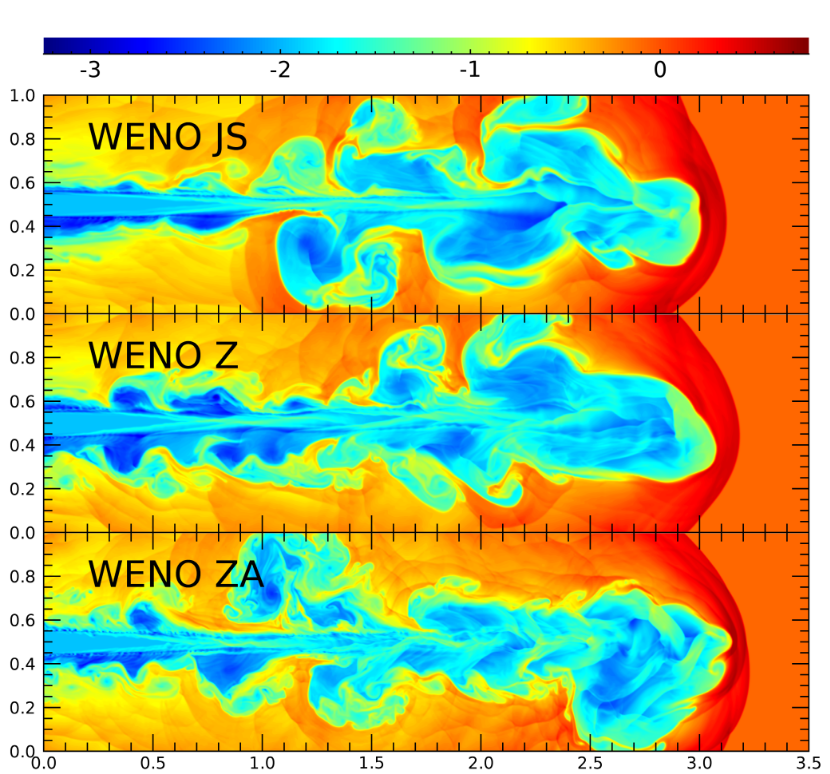
\includegraphics[width=0.95\textwidth]{Figuras/Introduccion/jet_ejemplo_2.png}
    \end{center}
    \caption{Mapa de densidad ($\log \rho$) del jet con CFL = 0.8, con un dominio computacional $\left[0, 3.5\right] \times \left[0, 1\right]$, con una resolución de 1050$\times$300 píxeles. Adaptado de la Figura 8 
    de \citet{Seo2021}.}
    \label{fig:jet_ejemplo_2}
\end{figure}

%--------------------------------------------------------------------------
%Ejemplo de estudio de jets relativistas en el marco de AGNs.
%--------------------------------------------------------------------------
En la Figura \ref{fig:jet_agn} se muestra la evolución de un jet relativista emitido desde un AGN y el cual se mueve a través del medio interestelar \citep{2011ApJ...743...42P}. El jet se inyecta desde un 
radio inicial de 100 pc con $\rho_j = 8.3 \times 10^{-29} \, \text{g}\,\text{cm}^{-1}$ y $v_j = 0.984$~c (y una relación de densidad entre el material del jet y el entorno de $\rho_j / \rho_a = 5\times10^{-4}$). De este modo, 
el jet se lanza con una luminosidad de $10^{46} \, \text{erg} \, \text{s}^{-1}$. Las condiciones de frontera, son la reflexión en la base del jet, así como en el eje y outflow al final del dominio en 
las direcciones axial y radial. Para detalles de las fronteras consulte el apéndice \ref{aped.B}. En el panel izquierdo se muestra el logaritmo de densidad al tiempo t = 1.1 Myr\footnote{$10^6$ años} con un largo de 900 Kpc. 
El capullo mide aproximadamente 400 Kpc, tiene una densidad de masa del 
orden de $\sim10^{-28}-10^{-30} \text{g} \, \text{cm}^{-3}$. Además, se tiene turbulencia y hay pequeñas cavidades dentro del capullo con $\sim10^{-32} \text{g} \, \text{cm}^{-3}$. En el panel derecho, el cual es un reflejo
del izquierdo pero tomando en 
cuenta la temperatura, los patrones de turbulencia también son visibles y las zonas menos densas son las más calientes (alcanzando $\sim 10^9$K). A escalas de parsecs, los jets de los AGNs siguen siendo altamente colimados y 
se mueven a velocidades cercanas a la de la luz.

\begin{figure}
  \begin{center}
    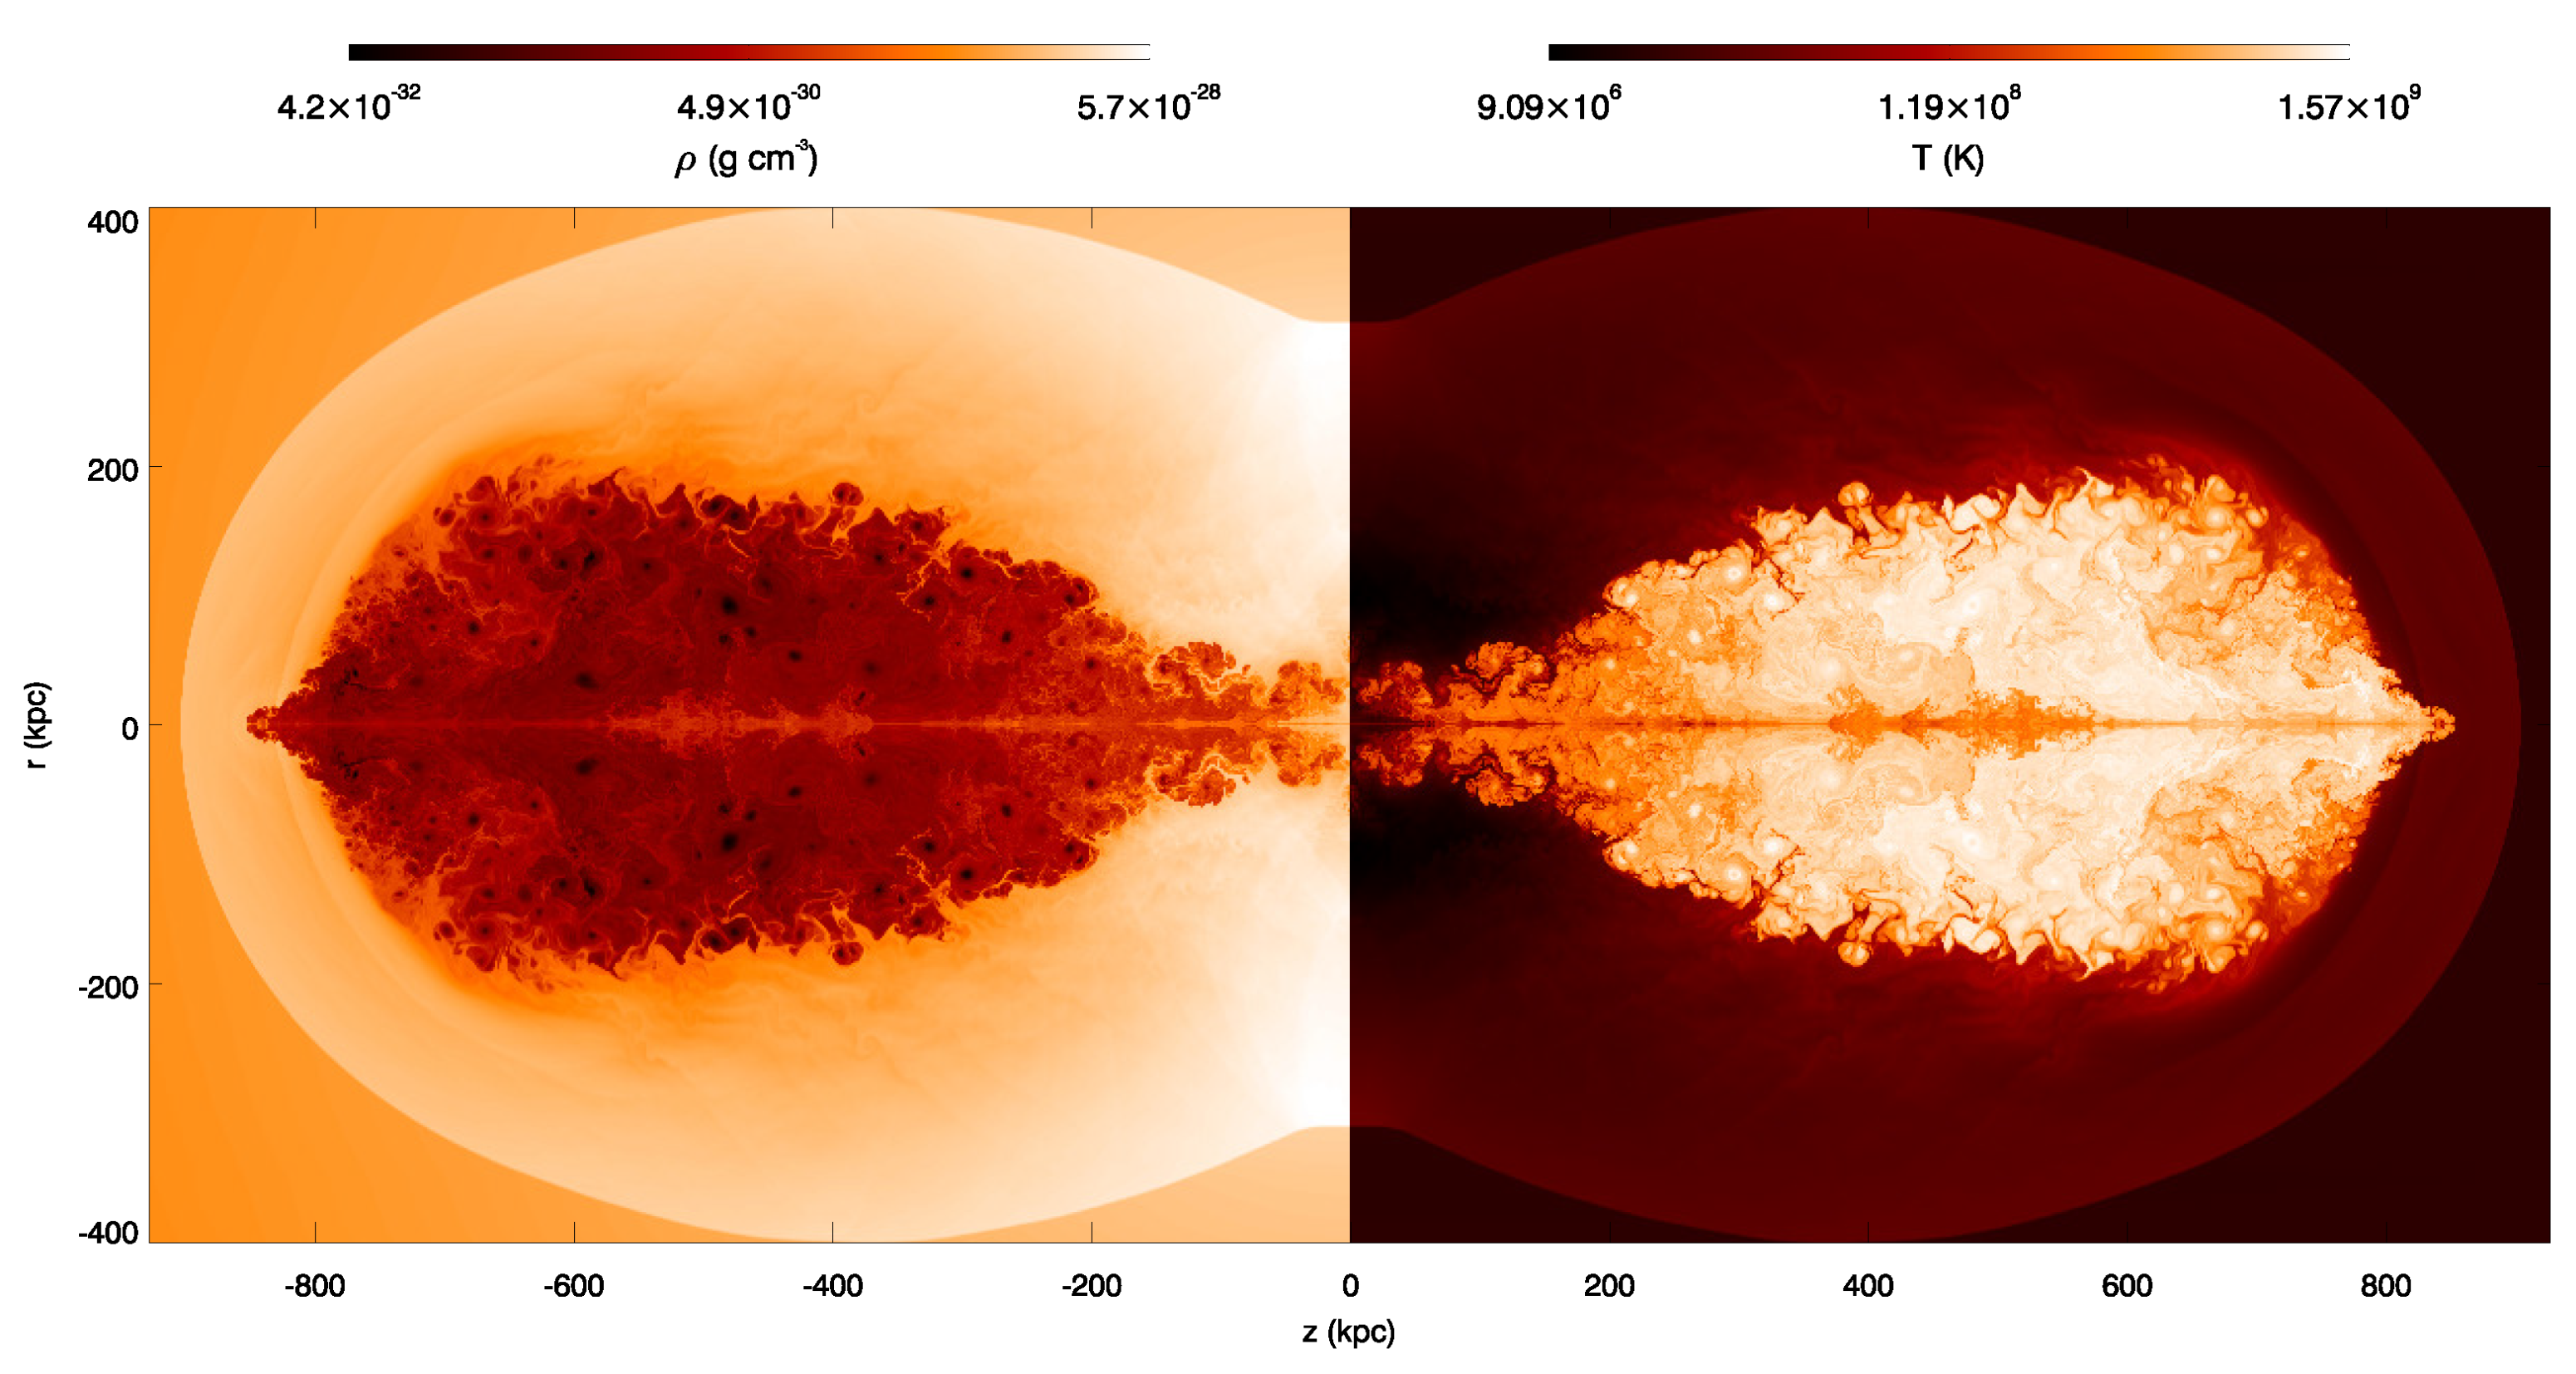
\includegraphics[width=0.95\textwidth]{Figuras/Introduccion/jet_agn.png}
  \end{center}
  \caption{Mapa del logaritmo de densidad (izquierda) y temperatura (derecha) al tiempo t = 1.1 Myr. Las figuras muestran una imagen reflejada alrededor del eje de simetría, donde se inyecta un jet con un radio inicial 
  de 100 pc con velocidades de flujo $v_j = 0.984$~c y una densidad $\rho_j = 8.3 \times 10^{-29} \, \text{g} \,\text{cm}^{-3}$. Adaptado de la Figura 8 de \citet{Marti2019}.}
  \label{fig:jet_agn}
\end{figure}



%--------------------------------------------------------------------------
%Ejemplo de estudio de jets relativistas en el marco de GRBs.
%--------------------------------------------------------------------------
El último ejemplo de simulaciones de jets relativistas es el estudio de \citet{JBEMGRB} en el cual se estudió la evolución de jets que son lanzados tras la fusión de estrellas de neutrones, así como en el  marco de los Colapsares. En la Figura~\ref{fig:jet_models} se muestra la evolución de distintos jets relativista a través de medios producidos tras la fusión de dos estrellas de neutrones (paneles de arriba) o 
a través de la envolvente de un Colapsar (paneles de abajo). El jet, que se lanza a través del medio producido tras la fusión de las dos estrellas de neutrones, tiene una luminosidad 
de $L_{\rm iso, 0} = 5.0 \times10^{50}$~erg~s$^{-1}$, un ángulo de apertura de $\theta_0=6.8^{\circ}$ (panel de arriba a la izquierda) o de $\theta_0=18.8^{\circ}$ (panel de arriba a la derecha). Es 
lanzado dentro de un radio de inyección $r_{in}=1.2\times10^{8}$~cm, y atraviesa un medio con masa de $M_{m} = 0.02 M_{\odot}$ que se mueve con velocidad $v_{m} = 0.34$~c (ver Cuadro~\ref{table:jet_models} para más detalles). 
El jet que se lanza dentro del Colapsar tiene una luminosidad de $L_{\rm iso, 0} = 7.83 \times10^{52}$~erg~s$^{-1}$ con ángulo de apertura de $\theta_0=9.2^{\circ}$ (panel de abajo a la izquierda), o una 
luminosidad de $L_{\rm iso, 0} = 1.27 \times10^{52}$~erg~s$^{-1}$ y ángulo de apertura de $\theta_0=22.9^{\circ}$ (panel de abajo a la derecha), los cuales son lanzados dentro de un radio de inyección $r_{in}=10^{9}$~cm, 
atravesando un medio que está en reposo y cuya masa es de $M_{m} = 13.95 M_{\odot}$.
\begin{figure} 
  \centering
    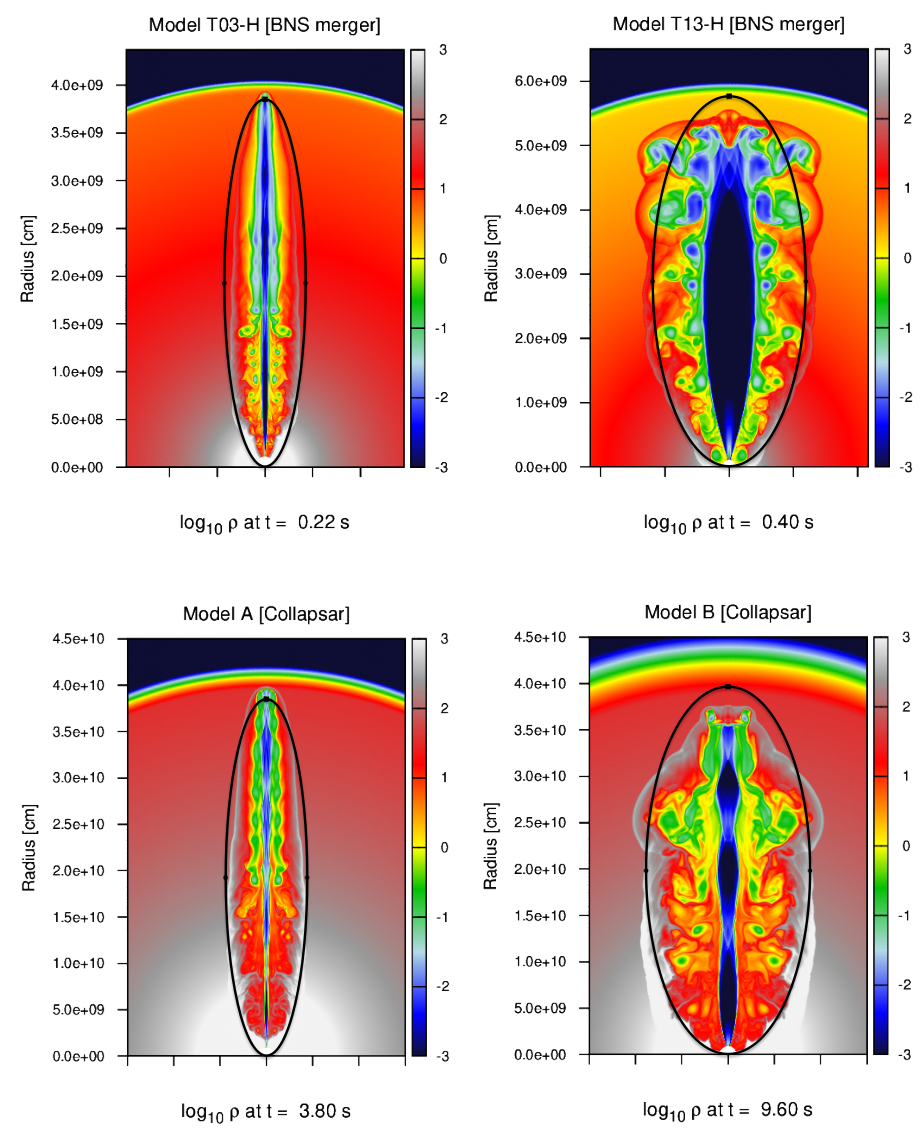
\includegraphics[width=0.7\textwidth]{Figuras/Introduccion/jet_models.png}
  \caption{Mapa de densidad del jet, donde los paneles de arriba muestran ambientes de una fusión de estrellas de neutrones, mientras que los paneles de abajo muestran para los Colapsares. Adaptado de la Figura 5 de
  \citet{JBEMGRB}.}
  \label{fig:jet_models}
\end{figure}
El panel de arriba a la izquierda de la Figura~\ref{fig:jet_models} muestra que para el tiempo $t = 0.22$~s el jet relativista y colimado ha avanzado una distancia de $3.75 \times 10^9 \, \text{cm}$ a través 
del medio producido tras la fusión de dos estrellas de neutrones. Para el tiempo final el capullo tiene un ancho de $3.75 \times 10^9 \, \text{cm}$. El capullo tiene una densidad que se encuentra dentro 
de $\sim10^{-1}-10^{2} ~cm^{-3}$. También se observa el jet en el centro del capullo en el cual la densidad disminuye a valores cercanos a $\sim 10^{-1}-10^{3} ~cm^{-3}$. Otro aspecto a tomar es que hay una mayor 
turbulencia cerca del radio de 
inyección y disminuye conforme el jet se va alejando. El jet se mantiene con un ancho aproximado de jet de $\sim 0.05 \times 10^9 \, \text{cm}$. El panel de arriba a la derecha muestra como el jet relativista menos 
colimado tarda casi el doble del tiempo en llegar a la misma distancia que el caso anterior (el jet colimado). Para el tiempo $t = 0.40$~s el capullo tiene $\sim 1.0 \times 10^9 \, \text{cm}$ de ancho. El jet no es 
completamente colimado, debido a que forma un óvalo y alcanza un ancho máximo de $0.3 \times 10^9 \, \text{cm}$ a una altura de $3.0 \times 10^9 \, \text{cm}$. El jet menos colimado muestra una mayor 
turbulencia (comparado con el más colimado), y la turbulencia es más caótica conforme el jet se aleja del radio de inyección. La densidad del capullo es menos densa, ya que hay más regiones con densidades 
$\sim 10^{-1} ~cm^{-3}$. El jet es más ancho y tiene densidades $\sim 10^{-3} ~cm^{-3}$.
% \Selene{Nota general: Puedes mejorar la redacción si estas comparando dos cosas, en todo este parrafo me perdí. Quiza podrías hacer una tabla comparativa}
% \Selene{Las referencias a las figuras son confusas, creo que deberias poner la referencia de las figuras siempre, ya que tus descripciones son largas. Pero esto es porque te hace falta posicionar mejor las tablas y 
% figuras, de modo que tu texto quede bien acomodado.}


El panel de abajo a la izquierda de la Figura~\ref{fig:jet_models} muestra el tiempo final de la evolución de un jet relativista y colimado a través de un Colapsar al tiempo $t = 3.8$~s. Su largo es de
$3.75 \times 10^{10} \, \text{cm}$. El jet es completamente colimado con un ancho de $0.05 \times 10^{10} \, \text{cm}$. A diferencia de los jets moviéndose a través de un medio formado tras la fusión de estrellas de 
neutrones, el borde del capullo tiene densidades que alcanzan $\sim10^{2}-10^{3} ~cm^{-3}$, además el capullo presenta más turbulencia conforme incrementa la distancia desde el radio de inyección. El jet tiene densidades 
del orden de $\sim 10^{-2}-10^{-1} ~cm^{-3}$. El panel de abajo a la derecha muestra nuevamente como los jets menos colimados tardan más tiempo en llegar a la misma posición que un jet colimado. En este caso el jet menos 
colimado requiere de $t = 9.60$~s para llegar a jet con un largo de $\sim 3.75 \times 10^9 \, \text{cm}$. El ancho del jet es de $0.1 \times 10^{10} \, \text{cm}$ y presenta una mayor densidad alrededor
del capullo con $\sim10^{3} ~cm^{-3}$. El capullo mide $1 \times 10^{10} \, \text{cm}$ y muestra choques de colimación en los puntos $1.5 \times 10^{10} \, \text{cm}$, $2.5 \times 10^{10} \, \text{cm}$ 
y $3.5 \times 10^{10} \, \text{cm}$. Queda claro como las características del jet (luminosidad, ángulo de apertura, etc.) así como las condiciones del medio a través del cual el o los jets se mueven afectan la 
evolución y morfología del mismo.

\begin{table}
  \begin{center}
    \begin{tabular}{ c c c c c c c} 
      \hline
      Modelo & Tipo                          & $\text{M}_{m} [\text{M}_{\bigodot}]$  & $\theta_0 [\text{grad}]$ & $\text{L}_{\text{iso},0}  [\text{erg}\,s^{-1}]$ & $r_{in} $ [cm]             & $v_m$ [c]               \\
      \hline
      T-03H  & Estrella Binaria de Neutrones & 0.02                                  &    6.8                   &               $5.0   \times 10^{50}$            &     $1.2 \times 10^8$      &   0.34  \\ 
      T-12H  & Estrella Binaria de Neutrones & 0.02                                  &    18.8                  &               $5.0   \times 10^{50}$            &     $1.2 \times 10^8$      &   0.34  \\ 
      A      & Colapsar                      & 13.950                                &    9.2                   &               $7.83  \times 10^{52}$            &     $10^9$                 &       0                 \\ 
      B      & Colapsar                      & 13.950                                &    22.9                  &               $1.27  \times 10^{52}$            &     $10^9$                 &       0                 \\ 
    \end{tabular}
  \caption{Valores que se usa las simulaciones de la Figura \ref{fig:jet_models} donde $\text{M}_{\bigodot}$ son masas solares, $\theta$ es el ángulo de apertura inicial, \emph{L} es la luminosidad isotrópica inicial,
  $r_{\text{in}}$ es el radio de inyección del jet y $v_m$ la velocidad del medio ambiente.} \label{table:jet_models}
  \end{center}
\end{table}

%----------------------------------------------------------------------------------
\section{Estudio de un jet relativista en dos dimensiones (Mignone \& Bodo, 2005).}
%----------------------------------------------------------------------------------
Uno de los objetivos de esta tesis es crear un código HD y RHD y lograr estudiar la evolución de un jet RHD. Para lo anterior se va a buscar reproducir los resultados del estudio de \citet{MB-HLLC-I} en 
que estudiaron la evolución de un jet relativista en dos dimensiones (ver Figura \ref{fig:jet_mignone}). 

Los valores que usaron para poder simular el jet relativista 2D (axisimétrico y en coordenadas cilíndricas), fueron los siguientes:
\begin{equation}
  \left(\rho, v_{r}, v_{z}, p\right)=\left\{\begin{array}{ll}
  \left(0.1,0,0.99,10^{-2}\right) & \text { para } r, z<1 \\
  \left(10,0,0,10^{-2}\right) & \text { caso contrario, }
  \end{array}\right.
\end{equation}
donde $\rho$ es la densidad, $v_r$ es la velocidad radial, $v_z$ es la velocidad sobre el eje z y $p$ es la presión. El índice adiabático\footnote{Razón entre el calor específico
a presión constante $C_p$ y calor específico a volumen constante $C_v$. Lo denotaremos como $\Gamma$.} que usaron fue $\Gamma = 5/3$ con un número de Courant $Co = 0.5$. 
Los métodos que emplearon fueron el método de HLL y HLLC (para más información ver la sección \ref{secc:HLL}). El tiempo de integración fue de $t = 80$ con condiciones de frontera \emph{outflow} excepto donde se 
inyecta el jet. La velocidad de avance promedio  del jet fue de 0.39 con una resolución de 240$\times$700 píxeles. 

La figura de arriba de \ref{fig:jet_mignone} muestra la morfología del jet a t=40, mientras que la de abajo a t=80. En ambas figuras el panel de arriba (i.e. el dominio positivo en Y) muestra el 
caso cuando la simulación se hizo utilizando el esquema HLLC. Por otro lado, el panel del abajo (i.e. el dominio negativo en Y) muestra el caso cuando se usó el esquema HLL.
\begin{figure}
  \begin{center}
    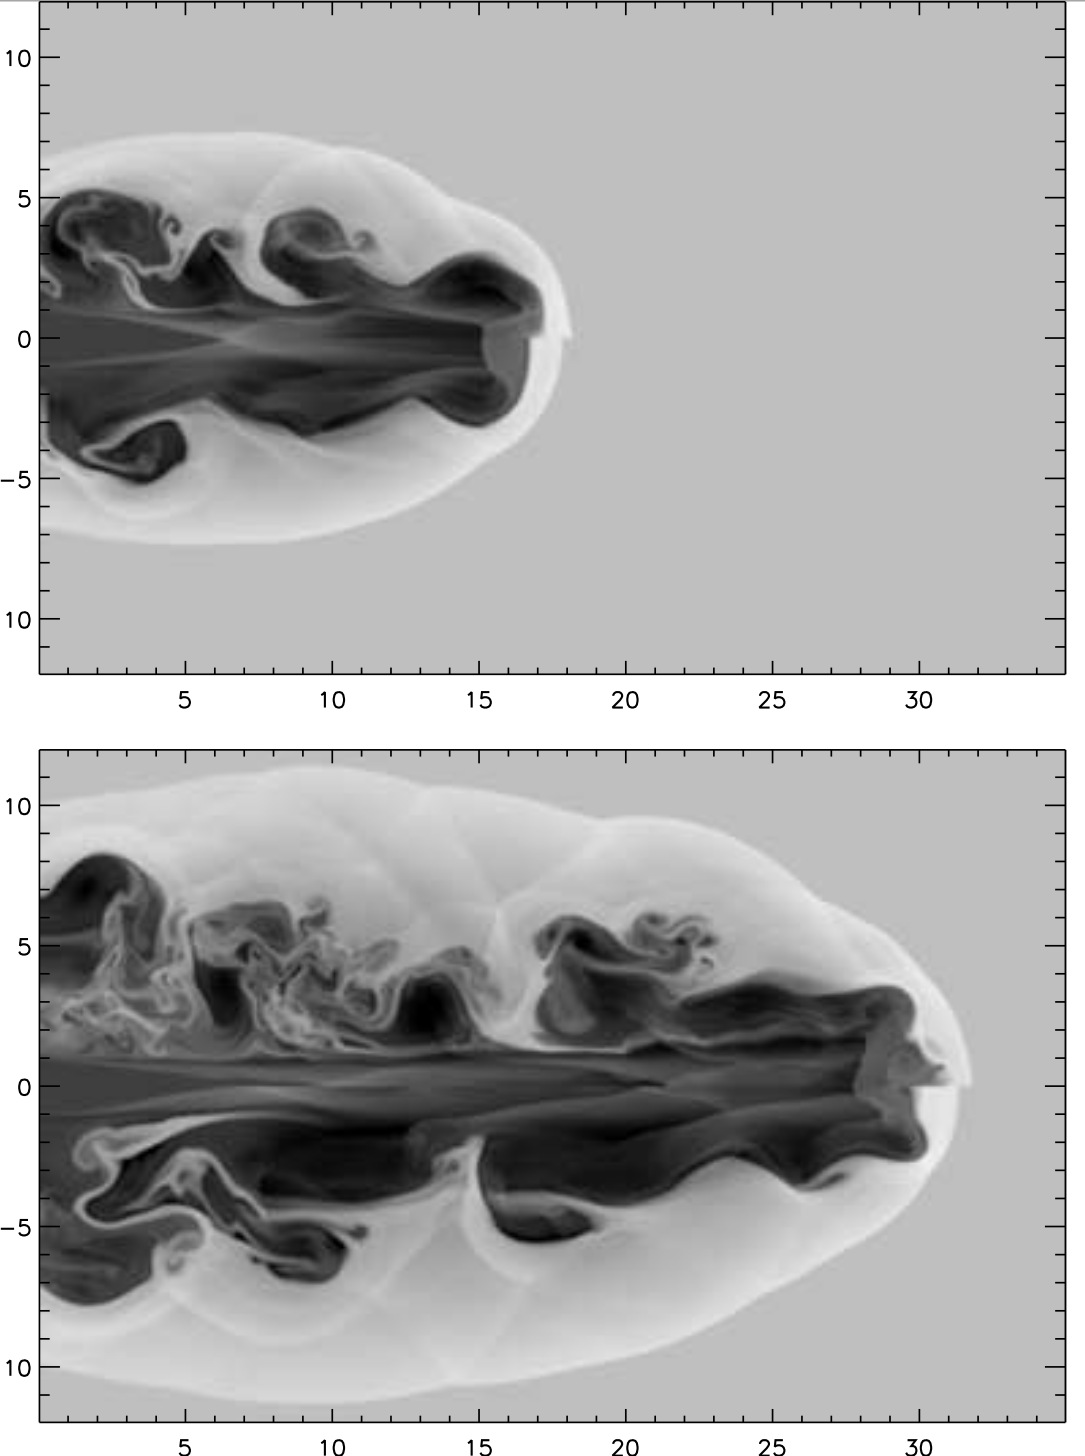
\includegraphics[width=0.5\textwidth]{Figuras/Introduccion/jet_mignone.png}
  \end{center}
  \caption{Logaritmo de la densidad de la masa en reposo para un jet relativista. El panel de arriba muestra el jet al tiempo t=40, mientras que el de abajo al tiempo t = 80.
  La mitad de  (de ambos paneles) muestra la simulación hecha con el esquema HLLC, mientras que la parte de abajo muestra para el esquema HLL.
  La resolución fue de 240$\times$700 píxeles. Adaptado de la Figura 12 de \citet{MB-HLLC-I}}
  \label{fig:jet_mignone}
\end{figure}

El panel de arriba muestra cómo para t=40, cuando se usa el método de HLLC, el jet tiene un tamaño sobre el eje radial de $\sim$19 unidades y un ancho de $\sim$5 unidades, mientras el capullo tiene un 
ancho máximo de $\sim$7 unidades. Para el caso, en el que se usa HLL, el jet tiene un tamaño de $\sim$18 unidades, un grosor de $\sim$5 unidades, y el capullo alcanza una anchura de $\sim$4 unidades. El caso HLL presenta 
una menor turbulencia con respecto a HLLC.
Para el panel de abajo (a t=80), en el caso de HLLC, presenta un largo de $\sim$32 unidades, un ancho es de $\sim$7 unidades y su capullo tiene una anchura de $\sim$11 unidades. Para el caso en que se usa HLL, el largo 
y ancho miden $\sim$31.5 y $\sim$8 respectivamente, mientras que el capullo presenta un tamaño de $\sim$11.5 unidades. Nuevamente, el caso HLL presenta menos turbulencia que el caso HLLC.
% \Selene{No sé si tu asesor o algún sinodal te guió para la redacción, si esta es tu introducción, para mi gusto tiene muchos datos técnicos que desconozco y siento que no me introduce, pero si tu crees que las personas que leerán esta tesis, especialistas en el tema no tendrán duda entonces esta bien.}
% \Selene{Sería genial que añadas una descripción de lo que vendrá en cada capitulo.}
% \Selene{Estas son algunas preguntas que me plantee para mi tesis, ojala te sirvan, \\
% - Responder a las siguientes cuestiones:\\
% ¿Cuáles son los antecedentes?
% ¿Cuál es el problema que responde \ resuelve mi trabajo?
% ¿Cómo se contribuye a la solución?
% ¿Cuáles son mis objetivos generales? --> Está si la respondes así que Ok :) }
%--------------------------------------------------------------------------
\section{Objetivos de la tesis}
%--------------------------------------------------------------------------
Los objetivos de esta tesis se enlistan a continuación:
\begin{itemize}
  \item Desarrollar un código que sea capaz de resolver numéricamente las ecuaciones de la hidrodinámica, tanto para los casos newtonianos (HD) así como los relativistas (RHD) en una (1D) y dos dimensiones (2D). 
  
  \item Incorporar los resolvedores numéricos Lax y HLL en el código (tanto en el HD como en el RHD).
  
  \item Verificar que el código HD funcione correctamente por medio de distintos problemas físicos que tengan solución analítica (en 1D y 2D). Comparar los resultados usando los métodos de Lax y HLL.

  \item Verificar que el código RHD funcione correctamente por medio de distintos problemas físicos que tengan solución analítica (en 1D y 2D). Comparar los resultados usando los métodos de Lax y HLL.
  
  \item Estudiar la evolución de un jet 2D relativista a través de un medio constante. Se reproducirá el estudio de \citet{MB-HLLC-I}, y se compararán los resultados obtenidos.

  \item Estudiar la evolución de un jet 2D relativista a través de distintos medios variables ($\rho \propto R^{-n}$, con $n=1, 2, 3$) y se compararán los resultados contra el caso en el que jet se mueve en un medio constante.

\end{itemize}





\chapter{Teoría}

% Los GRBs, ya sean largos o cortos, que se originan en el medio interestelar, se pueden describir como un fluido sin viscosidad y estos pueden ser descritos bajo
Los jets, ya sea que provengan de GRBs o AGNs, se pueden describir como un fluido sin viscosidad %AQUI HAY QUE ACLARAR ESTA LÍNEA
y estos pueden ser descritos bajo las ecuaciones de la hidrodinámica.
Para describir un sistema de partículas como un fluido bajo ciertas condiciones, uno debe de conocer que el camino libre medio debe de ser mucho más pequeño que la escala de longitud de las 
fluctuaciones de las variables macroscópicas \citep{LeVeque1998}.

\begin{equation}
\lambda_{mfp} \ll L.
\end{equation}

El tiempo entre las colisiones debe de ser pequeño comparado con la escala del tiempo de los cambios en el fluido.
\begin{equation}
t_{c} \ll t_f.
\end{equation}

La distancia media entre las partículas tiene que ser más pequeña que la longitud de escala de las variables macroscópicas.

\begin{equation}
l = n^{-1/3} \ll L.
\end{equation}



\section{Ecuaciones de la hidrodinámica}\label{sec:Ecuacioneshidrodinamica}

Considerando una serie de elementos de volumen fijos \citep{Clarke2007}, las ecuaciones que describen el movimiento de un fluido sin considerar efectos viscosos son:

La conservación de masa: 
\begin{equation} \label{conservación_masa_hidrodinamica}
\dfrac{\partial \rho }{\partial t} + \nabla \cdot \left( \rho \mathbf{u} \right)=0.
\end{equation}

El momento:
\begin{equation}  \label{conservacion_momento_hidrodinamica}
\dfrac{\partial \left( \rho \mathbf{u} \right) }{\partial t}+ \nabla \cdot \left( \rho \mathbf{u u} \right) + \nabla p = \mathbf{f_{ext}}.
\end{equation}

Ecuación de la energía:

\begin{equation} \label{conservacion_energia_hidrodinamica}
\dfrac{\partial e }{\partial t} + \nabla \cdot \left[ \mathbf{u} \left( e+p \right) \right] =G-L+\mathbf{f_{ext} \cdot \mathbf{u}}.
\end{equation}

Ecuación de estado:
\begin{equation}
e=\frac{1}{2} \rho \mathbf{u}^{2} + \frac{p}{\Gamma - 1}.
\end{equation}

Donde $\rho$ es la densidad, $\mathbf{u}$ es el vector de la velocidad y $p$ es la presión.
Con estas ecuaciones podemos formar un sistema de 5 ecuaciones diferenciales parciales acopladas. En coordenadas cartesianas:

\begin{equation} \label{euler_cartesianas}
\dfrac{\partial \mathbf{U}}{\partial t}+\dfrac{\partial \mathbf{F}}{\partial x}+\dfrac{\partial \mathbf{G}}{\partial y}+\dfrac{\partial \mathbf{H}}{\partial z}= \mathbf{S}  ,
\end{equation}

\noindent donde:
\begin{center}


$\mathbf{U}=
\left(\begin{smallmatrix}
\rho \\
\rho u \\
\rho v \\
\rho w \\
e \\
\end{smallmatrix}\right)
$,
$\mathbf{F} =
\left(\begin{smallmatrix}
\rho u \\
\rho u^{2}+P \\
\rho uv \\
\rho uw \\
u(e+P) \\
\end{smallmatrix}\right)
$,
$\mathbf{G} =
\left(\begin{smallmatrix}
\rho v\\
\rho vu \\
\rho v^{2}+P \\
\rho vw \\
v(e+P) \\
\end{smallmatrix}\right)
$,
$\mathbf{H} =
\left(\begin{smallmatrix}
\rho w\\
\rho wu \\
\rho wv \\
\rho w^{2}+P \\
w(e+P) \\
\end{smallmatrix}\right)
$, 
$\mathbf{S} =
\left(\begin{smallmatrix}
0 \\
f_{x} \\
f_{y} \\
f_{z} \\
G-L+\textbf{f} \cdot \textbf{u} \\
\end{smallmatrix}\right)
$
\end{center}

El término $\mathbf{U}$ son las variables conservadas, los términos $\mathbf{F}$, $\mathbf{G}$, $\mathbf{H}$ son los fluidos en las direcciones $x$, $y$ y $z$ y $\mathbf{S}$ son los términos fuente. 
Para poder resolver computacionalmente estas ecuaciones diferenciales parciales vamos a utilizar el método de las volúmenes finitos y el método de Lax sin considerar los términos fuente, es decir, 
$\mathbf{S}=0$.

La implementación en el código se hará en 2 dimensiones, por lo que la variable \emph{H} que corresponde a los flujos en el eje z será cero. El bloque de código está en una subrutina llamada \emph{fluxes}, 
donde en el mismo bucle se desacoplan las primitivas para que queden en función de las conservadas. Cabe señalar que tanto en $f(4,i,j)$ y $g(4,i,j)$ se usa la
la variable conservada $u(4,i,j)$, ya que $u(4,i,j) = e$. 

\begin{lstlisting}[frame=single]

  f(1,i,j)=rho*vx
  f(2,i,j)=rho*vx*vx+P
  f(3,i,j)=rho*vx*vy
  f(4,i,j)=vx*(u(4,i,j)+P)

  g(1,i,j)=rho*vy
  g(2,i,j)=rho*vx*vy
  g(3,i,j)=rho*vy*vy+P
  g(4,i,j)=vy*(u(4,i,j)+P)

\end{lstlisting}

Las variables \emph{i}, \emph{j} corren sobre todo el dominio espacial dentro de un bucle, el término $\mathbf{H}$ no es incluido, dado que estamos en 2D. 
El término \emph{u} hace alusión a las variables conservadas.

\subsection{Desacoplamiento de las ecuaciones de la hidrodinámica}\label{subsec:DesacoplamientoEcuacionesHidrodinamica}

Al final del método de volúmenes finitos, obtenemos las variables conservadas (\emph{U}), pero para calcular los flujos de nuevo necesitamos recuperar las primitivas, es decir, calcular las variables primitivas 
$(\rho, \, u, \, v,\, w, \, p )$ en función de nuestras variables conservadas $(U_1, \, U_2, \, U_3, \, U_4, \, U_5)$.

Despejar la densidad es sencillo, ya que es directo, $U_1= \rho$ por lo tanto:

\begin{equation}\label{primitiva_densidad}
\rho = U_1.
\end{equation}

\noindent Para las velocidades $U_i=\rho \upsilon_i$, donde $i=2,3,4$ y $\upsilon_i=u,v,w$, nos da $\upsilon_i= U_i/ \rho$ y usando la ecuación \ref{primitiva_densidad} queda:

\begin{equation} \label{primitiva_velocidades}
\upsilon_i = U_1/U_i.
\end{equation}
Para la ecuación   de la energía $U_5=e$ combinando con la ecuación   de estado y la ecuación \ref{primitiva_velocidades} obtenemos:
\begin{equation}
P = \left( \Gamma - 1 \right) \left[ U_5 - \frac{U_1 \left( \sum_{i=2}^{4} U_1/U_i \right)^2}{2} \right].
\end{equation}

En el código se implementa de la siguiente manera.
Las variables \emph{i}, \emph{j} son contadores, y antes de que se calculen los flujos, se tienen que calcular las primitivas. Dado que el desacoplamiento se implementa directamente en la subrutina \emph{fluxes}, para 
que se puedan calcular los flujos.

\begin{lstlisting}[frame=single] 
  

    !Desacoplamiento de las primitivas
    rho = u (1,i,j)
    vx  = u(2,i,j)/rho
    vy  = u(3,i,j)/rho
    P   = (u(4,i,j)-0.5*rho*(vx**2+vy**2))*(gamma-1.)

\end{lstlisting}

\noindent Donde la variable \emph{u(4,i, j)} es la densidad de energía, ya que, como se recordará, se está en 2 dimensiones.
  
\section{Hidrodinámica relativista}
Los jets generalmente tienen velocidades relativistas, por lo que la parte newtoniana no nos va a servir, pero si como apoyo para poder pasar a la hidrodinámica relativista.
Esta parte se añadirá a los códigos que ya hemos generado previamente. Las próximas secciones abordarán cómo cambian nuestras primitivas, cómo afectan a nuestras variables conservadas y cómo las podemos 
desacoplar, así como varios ejemplos al cambiar varios valores de nuestros parámetros y de las condiciones iniciales.

\subsection{Primitivas}
Las ecuaciones que se tienen para flujos newtonianos se pueden modificar para hacerlas relativistas \citep{Marty1999, Landau1987}. Para esto vamos a partir de 2 ecuaciones importantes que son la ecuación de energía-momento y la ecuación de conservación 
de masa:

\begin{equation}\label{ecuacion_conservación_masa}
\left( \rho U^{\alpha} \right)_{, \alpha} =0 ,
\end{equation}

\begin{equation}\label{ecuacion_momento_energia}
T_{, \beta}^{\alpha \beta}=0 .
\end{equation}

\noindent De la ecuación \ref{ecuacion_conservación_masa} se tiene la cuadrivelocidad para un sistema de 
3 coordenadas y considerando a la velocidad de la luz como $c=1$ se puede ver como $U^{\mu}=\gamma \left( 1, \textbf{v}\right)$ y sustituyendo este resultado (en 2 dimensiones espaciales) tendremos las ecuaciones 
$U_1$, $F_1$ y $G_1$. Para la ecuación \ref{ecuacion_momento_energia} podemos escribir el tensor de energía-momento como $T^{\mu \nu} = \rho h U^{\mu} U^{\nu} + pg^{\mu \nu}$ y usando la métrica de Minkowski

\begin{equation}
\eta_{\alpha \beta}= 
\begin{pmatrix}
 -1 & 0 & 0 & 0 \\
 0 & -1 & 0 & 0 \\
 0 & 0 & -1 & 0 \\
 0 & 0 & 0 & 1 \\ 
\end{pmatrix},
\end{equation}

\noindent podemos escribir a $T^{\mu \nu}$ matricialmente como:

\begin{equation}
T^{\mu \nu} =
\begin{pmatrix}
\rho h \gamma^2-p & \rho h \gamma^2 v_{x}  & \rho h \gamma^2 v_{y} & \rho h \gamma^2 v_{z} \\

\rho h \gamma^2 v_{x} & \rho h \gamma^2 v_{x}^{2}+p & \rho h \gamma^2 v_{x}v_{y} &  \rho h \gamma^2 v_{x}v_{z} \\

\rho h \gamma^2 v_{y} & \rho h \gamma^2 v_{y}v_{x} & \rho h \gamma^2 v_{y}^{2}+p & \rho h \gamma^2 v_{y}v_{z}\\

\rho h \gamma^2 v_{z} & \rho h \gamma^2 v_{z}v_{x} & \rho h \gamma^2 v_{z}v_{y} & \rho h \gamma^2 v_{z}^2 + p

\end{pmatrix} .
\end{equation}
Entonces las variables conservadas quedarían de la siguiente manera:
\begin{align}
u_{1}& = \rho \gamma \\ 
u_{2}& = \rho v_{x} \gamma^{2} h \\ 
u_{3}& = \rho v_{y} \gamma^{2} h \\ 
u_{4}& = \rho \gamma^{2} h - p 
\end{align}

\noindent donde $\rho$ es la densidad, $\gamma$ es el factor de Lorentz, $v_{x}$ y $v_{y}$ son las velocidades de los flujos (en 2 dimensiones, pero se puede extender esto a 3 sin ningún problema), 
$h$ es la entalpía  y $p$ es la presión. Para los flujos quedan de la siguiente manera:
\begin{align}
F_{1}& = \rho v_{x} \gamma \\ 
F_{2}& = \rho v_{x} v_{x} \gamma^{2} h + p\\ 
F_{3}& = \rho v_{x} v_{y} \gamma^{2} h \\ 
F_{4}& = \rho v_{x} \gamma^{2} h 
\end{align}

\begin{align}
G_{1}& = \rho v_{y} \gamma \\ 
G_{2}& = \rho v_{y} v_{x} \gamma^{2} h \\ 
G_{3}& = \rho v_{y} v_{y} \gamma^{2} h + p\\ 
G_{4}& = \rho v_{y} \gamma^{2} h .
\end{align}


La implementación en el código es de la siguiente manera, el factor de Lorentz $\gamma$ es la variable $lor$, $h$ la entalpía, al igual que en la hidrodinámica newtoniana solo se considerará 2 dimensiones:

\begin{lstlisting}[frame=single]
  lor=1/sqrt(1-(vx**2+vy**2))
  h=1.+gamma/(gamma-1.)*P/rho
  
  f(1,i,j)=rho*vx*lor
  f(2,i,j)=rho*vx*vx*lor**2*h+P
  f(3,i,j)=rho*vx*vy*lor**2*h
  f(4,i,j)=rho*vx*lor**2*h

  g(1,i,j)=rho*vy*lor
  g(2,i,j)=rho*vx*vy*lor**2*h
  g(3,i,j)=rho*vy*vy*lor**2*h+P
  g(4,i,j)=rho*vy*lor**2*h

\end{lstlisting}

A diferencia de los flujos newtonianos, para los flujos relativistas se tienen que calcular antes el factor de Lorentz \emph{lor} y la entalpía \emph{h},
las variables \emph{i}, \emph{j} son contadores sobre el espacio.

\subsection{Desacoplamiento de las ecuaciones de la hidrodinámica relativista} \label{Cap_Desacoplamiento_de_las_ecuaciones_de_la_hidrodinámica_relativista}
Para poder desacoplar las ecuaciones, se partirá de la relación de las densidades de energía total y del módulo de los momentos \citep{McKinney2007}. 

\begin{equation}\label{ecuación  _de_energia}
  e=W-p ,
\end{equation}

\begin{equation}\label{modulos de los momentos}
\abs{m}^2= W^{2}\abs{v}^{2}
\end{equation}

\noindent donde $W=D h \gamma$ y $D=\rho \gamma$. Para evitar errores en el límite no relativista se debe resolver la ecuación conservada restando la densidad de masa 
a la energía para definir una nueva variable conservada ($e^{'}=e-D$). Para las cancelaciones en el límite ultra-relativista basados en $\gamma \abs{v^2}$ que se tiene cuando $\abs{v} \rightarrow 1$, se debe de crear 
otra variable, que en este caso seria $\abs{u}^2=\gamma \abs{v^2}$ e introduciendo las variables $W^{'}=W-D$, podemos reescribir la última ecuación de la siguiente manera:
\begin{eqnarray*}
 W^{'}& = &D(h \gamma -1)\\
&=& D\left[ \left(1-\epsilon+ \frac{p}{\rho}\right) \gamma - 1 \right]\\
&=& D \left(\gamma-1 \right) \frac{\gamma+1}{\gamma+1}+\frac{D \gamma }{\rho}\left(\rho \epsilon + p \right).
\end{eqnarray*}

\noindent Recordando que $D=\rho \gamma$ y que a partir de la variable introducida $u^{2}$ podemos 
reescribir el factor de Lorentz como $\gamma^{2} = 1-u^{2}$

\begin{eqnarray}\label{W_prima}
\nonumber W^{'}&=&\frac{D u^{2}}{\gamma + 1}
+\frac{\rho\gamma \gamma}{ \rho }\left(\rho \epsilon + p \right)\\
&=& \frac{D u^{2}}{\gamma + 1} + \gamma^{2} \chi
\end{eqnarray}

\noindent donde $\chi=\rho \epsilon + p$, derivando con respecto a $W^{'}$ la ecuación \ref{ecuación  _de_energia} queda como
\begin{equation}\label{derivada_E_W}
\dfrac{de}{dW^{'}}=1-\dfrac{dp}{dW^{'}}.
\end{equation}

\noindent No se sabe como es la expresión $\dfrac{de}{dW^{'}}$, así que se asume que $p=p(\rho, \chi)$ por lo que podemos aplicar la regla de la cadena
\begin{equation}\label{cadena}
\dfrac{dp}{dW^{'}}=\dfrac{\partial p}{\partial\chi}\Bigg |_{\rho} \dfrac{d\chi}{dW^{'}} + \dfrac{\partial p}{\partial \rho}\Big |_{\chi} \dfrac{d \rho}{d W^{'}}.
\end{equation}

\noindent Para calcular $\dfrac{dp}{d\chi}$ tenemos que, por ser el caso de un gas ideal,
\begin{equation} \label{entalpía_función_presion_densidad}
h=1+\frac{\Gamma}{\Gamma-1}\frac{p}{\rho}
\end{equation}
donde $h$ también puede ser escrito como
\begin{equation}
h=1+\epsilon+\frac{p}{\rho}.
\end{equation}
Si combinamos estas 2 últimas ecuaciones podemos llegar a que 
\begin{equation}
p(\chi,\rho)=\frac{\Gamma-1}{\Gamma}\chi ,
\end{equation}

\noindent con lo que al derivar con respecto de $\chi$ nos da como resultado:
\begin{eqnarray}\label{der_presion}
& \dfrac{d p}{d \chi}&=\frac{\Gamma-1}{\Gamma} ,\\ &\dfrac{d p}{d \rho}&= 0.
\end{eqnarray}

\noindent De la ecuación \ref{W_prima} podemos despejar $\chi$, lo que queda como:
\begin{equation}
\chi=\frac{W^{'}}{\gamma}- \frac{D u^{2}}{(1+\gamma)\gamma^{2}}.
\end{equation}

\noindent Derivando implícitamente la ecuación \ref{W_prima} respecto a $W^{'}$ nos quedaría
\begin{eqnarray*}
W^{'}&=&D\left(\gamma-1 \right) + \chi \gamma^{2}\\%salto de linea
&=& D\left(\frac{1}{\sqrt{1-\nu^{2}}} -1\right)+\chi \dfrac{1}{1-\nu^{2}}, \\%salto de linea
\dfrac{d W^{'}}{d W^{'}} &=& D \dfrac{d (1-v^2)^{-1/2}}{d W^{'}}+\dfrac{d \chi}{dW^{'}}(1-v^2)^{-1}+\dfrac{d (1-v^2)^{-1} }{d W^{'}}\chi, \\  %salto de linea 
1 &=& \frac{D(1-v^2)^{-3/2}}{2} \dfrac{d v^{2}}{d W^{'}}+\dfrac{d \chi}{dW^{'}}(1-v^2)^{-1}+ \chi (1-v^2)^{-2}  \dfrac{d v^{2}}{d W^{'}}, \\ %salto de linea
\frac{1}{\gamma ^2} &=& \frac{D \gamma}{2} \dfrac{d v^{2}}{d W^{'}} + \dfrac{d \chi}{dW^{'}} + \chi \gamma^2 \dfrac{d v^2}{dW^{'}}. \\ %salto de linea
\end{eqnarray*}

\noindent Por lo tanto, la ecuación se puede escribir de la siguiente manera:

\begin{equation}\label{der_chi}
\dfrac{d \chi}{dW^{'}}=\frac{1}{\gamma^2}-\frac{\gamma}{2}(D-2\gamma \chi) \dfrac{d v^2}{dW^{'}},
\end{equation}

\noindent y para

\begin{equation}\label{der_rho}
\dfrac{d \rho}{d W^{'}}= D \dfrac{d\left(1/ \rho \right) }{d W^{'}} = - \frac{D \gamma}{2}  \dfrac{d v^2}{dW^{'}}.
\end{equation}

\noindent Despejando la ecuación \ref{modulos de los momentos} podemos llegar a escribir el módulo de la velocidad al cuadrado de la siguiente manera:
\begin{equation}
\abs{v^{2}} = \frac{\abs{m^{2}}}{W^{'}} 
\end{equation}
\noindent donde $m_i= \rho v_i \gamma h$ para $i=x,y$.

Se puede demostrar que $\dfrac{d \abs{v^2}}{W}=\dfrac{d \abs{v^2}}{W^{'}}$ para esto vamos a partir de lo siguiente: 
\begin{eqnarray*}
\abs{v^2}&=& \abs{m^{2}} \left(W^{'} + D \right)^{-2} \\
\dfrac{d \abs{v^2}}{d W^{'}} &=& \frac{-2 \abs{m}^2}{W^{'}+D^{3}} \\
&=& \frac{2 \abs{m}^2}{W^{3}} \\
&=& \dfrac{d \abs{v^2}}{d W^{'}},
\end{eqnarray*}

\noindent con lo que se puede decir que 

\begin{equation}\label{der_v2}
\dfrac{d\abs{v}^2}{d W^{'} }=-\frac{2 \abs{m}^{2}}{W^{3}}
\end{equation}
Con todo esto ya se sabe cuanto es lo que vale la ecuación \ref{derivada_E_W}, por lo que se puede usar el método de Newton-Raphson para poder encontrar $W^{'}$.
El método de Newton-Raphson es un algoritmo iterativo que se usa para encontrar raíces  de una función real:

\begin{equation} \label{eq_Newton_Raphson}
W^{'(k+1)}=W^{'}-\frac{f(W^{'})}{\dfrac{d f(W^{'})}{d W^{'}}}.
\end{equation}

De la ecuación de la densidad de energía, se puede usar como a la función a la que se quiere encontrar la raíz

\begin{equation} \label{ecuación_f}
f(W^{'})=W^{'}-e^{'}-p
\end{equation}

\noindent donde $e^{'}=W^{'}-p$ y que $\dfrac{d f(W^{'})}{d w} \equiv \dfrac{de}{dW^{'}}$ dado por la ecuación \ref{derivada_E_W}. 
Para iniciar el proceso de iteración se tiene que hacer una suposición. Para esto, con ayuda de las ecuaciones \ref{ecuación  _de_energia} 
y \ref{modulos de los momentos}, se puede llegar a que la presión es:
%===============================================================================================

\begin{equation} \label{presion_de_newton}
p=\frac{\abs{m}^{2}-W^{2}\abs{v}^{2}+4W^{2}-4eW}{4W}.
\end{equation}

Como se puede ver, el numerador es una función convexa cuadrática que depende $\abs{v}^{2}$ y $W$ y cumple con que $W$ este fuera del intervalo de las raíces positivas y negativas.
Al denominador de la  ecuación se puede encontrar $W$, ya que $\abs{v}^{2}=1-1/\gamma^{2}$. Suponiendo $\gamma \rightarrow \infty$ podemos despejar $W$

\begin{equation}\label{suposicion_de_W}
W=\frac{-(-2e)+\sqrt{(-2e)^{2}-(3)(\abs{m}^{2})}}{3}.
\end{equation}

Con esto ya se puede hacer las aproximaciones para obtener $W$, y se puede calcular las siguientes relaciones: 
\begin{eqnarray}
\abs{v}^{2} &=& \frac{\abs{m}^{2}}{W^{2}}\label{prim_v2},\\ 
u^{2}&=&\frac{\abs{v}^{2}}{1-\abs{v}^{2}}\label{u2},\\
\gamma &=& \sqrt{1+u^{2}}
\end{eqnarray}
y las nuevas primitivas.\\
Velocidades:
\begin{eqnarray}
v_{x}&=&\frac{u_{2}}{W},\\
v_{y}&=&\frac{u_{3}}{W}.\\
\end{eqnarray}

\noindent Densidad de masa: 
\begin{equation}
\rho=\frac{D}{\gamma}.
\end{equation}

\noindent Presión térmica:
\begin{eqnarray}
\chi&=&\frac{W-D}{\gamma^{2}}-\frac{D \abs{u}^{2}}{(1+\gamma)\gamma^{2}},\\
p&=&\frac{\Gamma-1}{\Gamma} \chi.
\end{eqnarray}

Aunque en el método newtoniano se podían desacoplar las ecuaciones sobre el mismo bucle, 
para el método relativista se tuvo que crear una subrutina para poder desacoplar las primitivas y así poder obtenerlas en función de las conservadas. 
La subrutina de desacoplamiento se llama \emph{uprim}, 
y ésta recibe un parámetro de entrada, que es la conservada \emph{u} y devuelve una variable primitiva. 
Las variables conservadas se reasignan a unas nuevas llamadas \emph{qu} para que se pueda usar la subrutina, una vez que se desacoplan, 
los valores de salida, éstas se reasignan a otras llamadas \emph{qpp}. Se tienen que reasignar dado que la subrutina pide números reales y no matrices.

\begin{lstlisting}[frame=single] 
        
    qu(1) = u(1,i,j)
    qu(2) = u(2,i,j)
    qu(3) = u(3,i,j)
    qu(4) = u(4,i,j)

    ! Desacoplamiento de las primitivas
    call uprim(u,qp)

    qpp(:,i,j)=qp

    rho = qpp(1, i,j)
    vx  = qpp(2, i,j)
    vy  = qpp(3, i,j)
    P   = qpp(4, i,j)


\end{lstlisting}

\noindent La subrutina de desacoplamiento para las variables conservadas que se mencionan en esta sección recibirá las variables conservadas
y devolverá las primitivas. La subrutina \emph{newrap} se usará en particular 
(ver apéndice \ref{ap_newrap}) para resolver la ecuación \ref{eq_Newton_Raphson}.

\begin{lstlisting} [frame=single]
  
  m2 = sum(qu(2:3)**2)               ! v^2

  call newrap(qu, w, m2)

  alpha = m2 / w**2   ! alpha < 1 !
  u2  = alpha/(1.0-alpha)

  lor = sqrt(1.0 + u2)

  ! velocities
  qp(2:3) = qu(2:3) / w

  ! determination of the mass density
  qp(1) = qu(1)/lor

  ! thermal pressure
  chi = (w - qu(1)*(1.0+u2/(lor+1.0)))/(1.0+u2)

  qp(4)   = (gamma - 1.0)/gamma * chi

  qp(4) =max(qp(4),1d-10*qp(1))
\end{lstlisting}

Las variables \emph{qp} mostradas en el código son las primitivas, mientras que las otras son auxiliares mostradas en el capítulo 
\ref{Cap_Desacoplamiento_de_las_ecuaciones_de_la_hidrodinámica_relativista}.


\section{Volúmenes finitos} \label{sec:Diferencias_finitas}
Ya se ha visto que ecuaciones describen la hidrodinámica, ahora toca resolverlas. Dado que analíticamente es difícil, se va a hacer computacionalmente, para 
eso se hará uso del método numérico de volúmenes finitos \citep{Duran2021}.
Si tenemos una función $f(x)$ diferenciable la podemos aproximar por el teorema de Taylor en la vecindad de un punto $x_0$ y si se conocen todas sus $n$ derivadas de la función $f(x)$ en el punto $x_0$ se puede 
aproximar de la siguiente manera

\begin{equation}\label{Serie_Taylor}
f\left( x_0 + \Delta x\right) = f\left( x_0 \right)+
\sum_n \frac{\left( \Delta x \right) ^2}{k!}f^{(k)} \left(x_0
\right)
\end{equation}

Si se trunca la serie de Taylor y se quitan los términos de segundo orden, se puede escribir la ecuación \ref{Serie_Taylor} como:

\begin{equation}
f\left( x_0 + \Delta x \right) = f(x_0) + \Delta x f^{(1)} (x_0) + O \left( \Delta x \right).
\end{equation}

\noindent Despejando $f(x_0)$ queda lo que se conoce como diferencias finitas hacia adelante
\begin{equation}\label{fwd}
f_{fwd}^{'}=\frac{f\left(x + \Delta x \right) - f(x) }{\Delta x}=\frac{f_{i+1}-f_{i}}{\Delta x}.
\end{equation}

\noindent También se puede hacer en el entorno $x_0- \Delta x$, siguiendo los mismos pasos anteriores se llega a lo que se le conoce como diferencias finitas hacia atrás


\begin{equation}\label{bwd}
f_{back}^{'}=\frac{f\left(x \right) - f(x - \Delta x) }{\Delta x}=\frac{f_{i}-f_{i-1}}{\Delta x}.
\end{equation}

\noindent Si se obtiene el promedio de las ecuaciones \ref{fwd} y \ref{bwd} se puede calcular la central:

\begin{equation} \label{Centrada}
f_{central}^{'}=\frac{f\left(x + \Delta x\right) - f(x - \Delta x) }{2\Delta x}=\frac{f_{i+1}-f_{i-1}}{2 \Delta x}
\end{equation}



\subsection{Lax-Friederichs}

Sí se considera la siguiente ecuación diferencial parcial \citep{Duchateau2002}

\begin{equation} \label{ecu_conser}
u_t+ f\left(u \right)_t=0.
\end{equation}

\noindent Un método conservativo para resolver este tipo de ecuación diferencial es 

\begin{equation}\label{esquema conservativo}
u_i^{n+1} = u_i^{n} -\frac{\Delta t}{\Delta x} \left(f_{i-\frac{1}{2}} - f_{i+\frac{1}{2}}\right)
\end{equation}



\noindent Sí se hace la siguiente elección de flujo 

\begin{equation}
f_{i+\frac{1}{2}} = f_{i+\frac{1}{2}} \left(
u_{i} , u_{i+1}\right) =\frac{1}{2} \left(f_{i} + f_{i+1} \right), 
\end{equation}

\noindent y para 

\begin{equation}
f_{i-\frac{1}{2}} = f_{i-\frac{1}{2}} \left(
u_{i} , u_{i-1}\right) =\frac{1}{2} \left(f_{i} - f_{i-1} \right) 
\end{equation}

\noindent y si se sustituye en la ecuación \ref{esquema conservativo} nos queda el siguiente resultado

\begin{equation}\label{ec_inestable}
u_i^{n+1} = u_i^{n} - \frac{1}{2}\frac{\Delta t}{\Delta x} \left(f_{i+1} - f_{i-1} \right).
\end{equation}

\noindent Pero esta solución es inestable, por el primer término del lado derecho de la ecuación, para hacerlo estable Peter Lax y Kurt Friedrichs sustituyeron este término, por $(u_{i+1}^n+u_{i-1}^n)/2$  por lo que se puede
reescribir la ecuación \ref{ec_inestable} como

\begin{equation}\label{ec_estable}
  u_{i,j}^{n+1} =(u_{i+1}^n+u_{i-1}^n)/2 + \frac{1}{2}\frac{\Delta t}{\Delta x} \left(f_{i+1} - f_{i-1} \right).
\end{equation}

\noindent Para 2 dimensiones sería

\begin{equation}\label{ec_estable}
  u_i^{n+1} =(u_{i+1,j}^n+u_{i-1,j}^n+u_{i,j+1}^n+u_{i,j-1}^n)/4 - \frac{1}{2}\frac{\Delta t}{\Delta x} \left(f_{i+1,j} - f_{i-1,j} \right)-\frac{1}{2}\frac{\Delta t}{\Delta y} \left(g_{i,j+1} - g_{i,j-1} \right).
\end{equation}

En el código, la implementación de la ecuación \ref{ec_estable} en 2 dimensiones es la siguiente

\begin{lstlisting} [frame=single]

  call fluxes(nx,ny,neq,gamma,u,f,g,bound)

  do i=1,nx
    do j=1,ny
      up(:,i,j)=0.25*( u(:,i-1,j)+u(:,i+1,j)+u(:,i,j-1)+u(:,i,j+1) ) &
                  -dtx*0.5*(f(:,i+1,j)-f(:,i-1,j) ) &
                  -dty*0.5*(g(:,i,j+1)-g(:,i,j-1) )
    end do
  end do
  
\end{lstlisting}

\noindent donde $\text{dtx} = \frac{\Delta t}{\Delta x}$, $\text{dty} = \frac{\Delta t}{\Delta y}$ y \emph{up} es la conservada posterior en el tiempo.



\subsection{HLL} \label{secc:HLL}
Antes de seguir con este método, se procedera a dar una breve descripción del problema de Riemann. Éste consiste en un problema de condiciones iniciales para una ecuación hiperbólica en derivadas parciales, la cual
se puede escribir matemáticamente de la siguiente manera: 

\begin{equation}
  \frac{\partial U}{\partial t}+\frac{\partial F}{\partial x}=0 \quad U=\left\{\begin{array}{l}
  U_{L}, \, x<x_{0} \\
  U_{R}, \, x>x_{0} 
  \end{array}\right.
\end{equation}

\noindent donde $U$ son las conservadas y $F$ son los flujos. Los valores de $U_{L}$ y $U_{R}$ representan los estados izquierda y derecha de un gas que esta separado por una membrana en el punto $x_0$ al tiempo 
inicial \citep{Lora2013}.
Para más detalles acerca de este problema consulte \citet{Toro1997}.



	Para usar el método de Harten-Van-Leer \citep{Toro1997} se tiene que definir el flujo numérico intercelda de Gudonov

\begin{equation}
F_{i+\frac{1}{2}}=F \left( U_{i+\frac{1}{2}} \right)
\end{equation}

\noindent para el cual $U_{i+\frac{1}{2}}(0)$ tiene la misma solución para $U_{i+\frac{1}{2}}(x/t)$ con lo que el problema de Riemann se reduce a:

\begin{equation} \label{ecuacion_discreta_conservada}
\begin{array}{ll}
U_t + F \left( U \right)_x = 0 \\
U \left(x,0 \right) = 
\left\lbrace
\begin{array}{rr}
U_L \quad \textup{si} \quad x<0  \\
U_R \quad \textup{si} \quad x>0.
\end{array}
\right.
\end{array}
\end{equation}

\begin{figure} %fuente de la imagen:libro del toro/
  \centering
    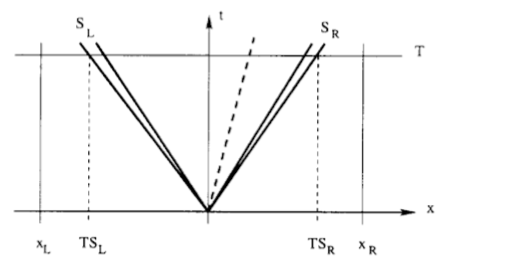
\includegraphics[width=0.5\textwidth]{Figuras/HLL_onda.png}
  \caption{Plano x-t que muestra un volumen definido. Adaptado de \citet{Toro1997}}.
  \label{fig:Plano x_t}
\end{figure}

\noindent Si se considera un volumen $\left[x_L, x_R \right]\times \left[ 0 , T \right]$, tales que $x_L \leq TS_L$ y $x_R \geq TS_R$ (ver Figura \ref{fig:Plano x_t}) donde $S_L$ y $S_R$ son las velocidades de las ondas más 
rápidas de los estados iniciales $U_L$ y $U_R$ respectivamente y $T$ es un tiempo definido. Y se usa la forma integral de la 
ecuación   \ref{ecuacion_discreta_conservada} en nuestro volumen definido $\left[x_L, x_R \right]\times \left[ 0 , T \right]$

\begin{equation*}\label{Forma_integral_conservadas}
\int_{x_L}^{x_R} \left[ U\left( x, T \right) -
 U\left( x, 0 \right) \right] dx = 
 \int_{0}^{T} \left[ F \left(U\left( x_L, t \right) \right) -
 F \left(U\left( x_R, t \right) \right) \right] dt, 
\end{equation*}
entonces
\begin{equation}\label{integral_consistencia}
\int_{x_L}^{x_R} U\left( x, T \right) dx =\int_{x_L}^{x_R} U\left( x, 0 \right) dx+
\int_{0}^{T}  F \left(U\left( x_L, t \right) \right)dt -
\int_{0}^{T}  F \left(U\left( x_R, t \right) \right) dt.
\end{equation}

\noindent Usando las condiciones de la ecuación \ref{ecuacion_discreta_conservada} se puede evaluar la integral

\begin{equation*}
\int_{x_L}^{x_R} U\left( x, T \right) dx = 
x_R U_R -x_L U_L+T F_L-T F_R
\end{equation*}
donde $F_L = F \left( U_L \right)$ y $F_R = F \left( U_R \right),$ 
entonces

\begin{equation}\label{Condición_de_consistencia}
\int_{x_L}^{x_R} U\left( x, T \right) dx = 
x_R U_R -x_L U_L+T \left( F_L- F_R \right).
\end{equation}

\noindent Si se separa la ecuación \ref{integral_consistencia} en 3 integrales de la siguiente manera:

\begin{equation}
\int_{x_L}^{x_R} U\left( x, T \right) dx = 
\int_{x_L}^{T S_L} U \left(x, T \right)dx+
\int_{T S_L}^{T S_R} U \left(x, T \right)dx+
\int_{T S_R}^{x_R} U \left(x, T \right)dx.
\end{equation}

\noindent Evaluando el tercer y el primer término en el lado derecho, obtenemos:

\begin{equation}\label{condicion_consistencia_2}
\int_{x_L}^{x_R} U\left( x, T \right) dx =
\int_{T S_L}^{T S_R} U \left(x, T \right)dx+
\left( T S_L - x_L \right) U_L+
\left( x_L - T S_R \right) U_R.
\end{equation}

\noindent Combinando la ecuación \ref{Condición_de_consistencia} y 
\ref{condicion_consistencia_2}

\begin{equation*}
x_R U_R -x_L U_L+T \left( F_L- F_R \right) =
\int_{T S_L}^{T S_R} U \left(x, T \right)dx+
\left( T S_L - x_L \right) U_L+
\left( x_L - T S_R \right) U_R.
\end{equation*}

\noindent Entonces 

\begin{equation*}
\int_{T S_L}^{T S_R} U \left(x, T \right)dx=
\left( T S_L - x_L \right) U_L+ x_L U_L +
\left( x_L - T S_R \right) U_R-x_R U_R -
T \left( F_L- F_R \right),
\end{equation*}

\noindent con lo que al final queda

\begin{equation} \label{ull_sin_promedio}
\int_{T S_L}^{T S_R} U \left(x, T \right)dx=
T \left( S_R U_R - S_L U_L + F_L - F_R \right).
\end{equation}

\noindent Dividiendo la ecuación \ref{ull_sin_promedio} por la diferencia de las velocidades máximas de las señales de las ondas, se obtiene el promedio de la función que está entre las velocidades de la onda, entonces

\begin{equation}
\frac{1}{T \left( S_R -S_L \right)}\int_{T S_L}^{T S_R} U \left(x, T \right)dx =
\frac{S_R U_R - S_L U_L + F_L - F_R}{S_R - S_L}.
\end{equation}

\noindent Si se conocen las velocidades de la onda, se puede escribir la ecuación como 

\begin{equation}\label{u_hll}
U^{hll} = \frac{S_R U_R - S_L U_L + F_L - F_R}{S_R - S_L}.
\end{equation}

\noindent Aplicando la forma integral (como en el caso de la ecuación \ref{Condición_de_consistencia}) al lado izquierdo del plano, se obtiene lo siguiente:

\begin{equation}
\int_{T S_L}^{0} U\left( x, T \right) dx = 
-T S_L U_L+T \left( F_L- F_{0L} \right)
\end{equation}
donde $F_{0L}$ es el flujo a lo largo del eje $t$. Si se despeja $F_{0L}$ queda lo siguiente:

\begin{equation}\label{ec F_0L}
F_{0L} = F_L - S_L U_L + \frac{1}{T}  \int_{T S_L}^{0} U\left( x, T \right) dx.
\end{equation}

\noindent Esta última ecuación servirá para calcular los flujos usando el método de Harten, Lax, van Leer, el cual dividían el plano en tres espacios alrededor de una interfase

\begin{figure} %fuente de la imagen:libro del toro/
  \centering
    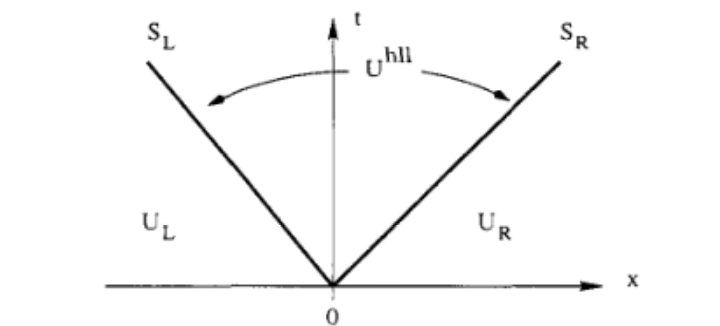
\includegraphics[width=0.5\textwidth]{Figuras/HLL.png}
  \caption{Aproximación de 3 estados distintos en el plano x-t, en el cual se trata de calcular los flujos en la región $U^{\text{hll}}$ limitados por las velocidades de señal de la onda.}
  \label{fig:HLL}
\end{figure}

\begin{equation}
  U(x, t)=\left\{\begin{array}{lll}
  U_{L} & \text { si } & \frac{x}{t}<S_{L} \\
  U_{h l l} & \text { si } & S_{t}<\frac{x}{t}<S_{R} \\
  U_{R} & \text { si } & \frac{x}{t}>S_{R}.
  \end{array}\right.
\end{equation}

Los flujos $F_R$ y $F_L$ pueden ser calculados directamente, ya que solo dependen de $U_R$ y $U_L$ respectivamente, pero $F_{hll} \neq F \left( U_{hll} \right)$, así que resolvemos la integral de 
la ecuación \ref{ec F_0L} para así obtener el flujo a través del eje t

\begin{equation*}
F_{hll} = F_L -S_L U_L+ \frac{1}{T}U_{hll}\left(0- TS_L\right).
\end{equation*}

\noindent Entonces
\begin{equation}\label{f_hll_1}
F_{hll} = F_L +S_L \left( U_{hll} -U_L \right).
\end{equation}

\noindent Si se sustituye \ref{u_hll} en \ref{f_hll_1} obtenemos

\begin{equation*}
F_{hll} = F_L +S_L \left( \frac{S_R U_R - S_L U_L + F_L - F_R}{S_R - S_L} -U_L \right),
\end{equation*}
entonces
\begin{equation*}
F_{hll} = \frac{F_L S_R -F_L S_L+S_L S_R U_R-S_L^2 U_L+S_L  F_L- S_L F_R-S_R S_L U_L + S_L^2 U_L}{S_R-S_L}.
\end{equation*}

\noindent Eliminando términos semejantes queda
\begin{equation}
F_{hll} = \frac{S_R F_L -S_L F_R + S_L S_R \left(U_R-U_L \right)}{S_R -S_L},
\end{equation}

\noindent con lo que el flujo intermedio de la celda de Godunov está dado por:


\begin{equation} \label{fluxesHLL}
  F_{i+\frac{1}{2}}^{h l l}=\left\{\begin{array}{l}
  F_{L} \quad \text { si } \quad 0 \leq S_{L} \\
  \frac{S_{R} F_{L}-S_{L} F_{R}+S_{L} S_{R}\left(U_{R}-U_{L}\right)}{S_{R}-S_{L}} \quad \text { si } \quad S_{L}  \leq 0 \leq S_{R} \\
  F_{R} \quad \text { si } \quad 0 \geq S_{R}.
  \end{array}\right.
\end{equation}

La implementación de esta parte se lleva a cabo en la subrutina \emph{ulax},

\begin{lstlisting} [frame=single]
  call fluxesHLL(fhll, ghll)
      
        do i=1,nx
          do j=1,ny
            up(:,i,j) = u(:,i,j)                                     &
                        + 0.5*dtx*(fhll(:,i-1,j)-fhll(:,i+1,j))      &
                        + 0.5*dty*(ghll(:,i,j-1)-ghll(:,i,j+1))
          end do
        end do

\end{lstlisting}

\noindent donde \emph{fhll} y \emph{ghll} son los flujos calculados con el método de HLL.
La subrutina llama a \emph{fluxesHll}, que es la subrutina que se encarga de calcular los flujos usando el método de HLL, el siguiente código solo es una parte
y solo calcula la ecuación \ref{fluxesHLL}, las variables $i$, $j$ refieren a todos los puntos de la malla, los subíndices \emph{l}, \emph{r}, \emph{u} y \emph{d}
significan izquierda, derecha, arriba y abajo respectivamente y \emph{S} son las velocidades de las ondas más rápidas de los estados iniciales \emph{U}. Para ver toda la subrutina completa ver el apéndice \ref{ap_newrap}.

\begin{lstlisting} [frame=single]
  do i=1,nx
  do j=1,ny
    
    if (0 .le. s_l(i,j)) then !less or equal 0<=sl
      fhll(:,i,j)=f_l(:, i,j)

    else if (s_l(i,j) .le. 0 .and. 0 .le. s_r(i,j)) then !sl<=0<=sr
  
      fhll(:,i,j)=(s_r(i,j)*f_l(:,i,j)-s_l(i,j)*f_r(:,i,j)+s_l(i,j)*s_r(i,j)*(u_r(:,i,j)-u_l(:,i,j)))/&
      (s_r(i,j)-s_l(i,j))


    else if (s_r(i,j) .le. 0) then !sr<=0
        fhll(:,i,j)=f_r(:,i,j)

    endif

    if(0 .le. s_d(i,j)) then
      ghll(:,i,j)= g_d(:,i,j)

    else if(s_d(i,j) .le. 0 .and. 0 .le. s_u(i,j)) then

      ghll(:,i,j)=(s_u(i,j)*g_d(:,i,j)-s_d(i,j)*g_u(:,i,j)+s_d(i,j)*s_u(i,j)*(u_u(:,i,j)-u_d(:,i,j)))/&
      (s_u(i,j)-s_d(i,j))

    else if(s_u(i,j) .le. 0) then
        ghll(:,i,j) = g_u(:,i,j)

    endif
  end do
end do
\end{lstlisting}



\section{Condiciones de salto}\label{sec:Condiciones_Salto}

\subsection{Rankine-Hugoniot}

Ya se ha visto cómo se resuelven las ecuaciones de la hidrodinámica, pero hay un problema: cuando un jet  choca contra el medio que lo rodea se genera una onda de choque. 
Esta onda de choque es una discontinuidad de la masa, presión y energía entre el jet y el medio que los rodea. Este problema se resuelve con las ecuaciones de 
Rankine-Hugoniot \citep{Prunty2019}.
Considerando las relaciones que hay entre los 2 estados que se forman durante una onda de choque. Supongamos que la onda de choque se mueve 
hacia la derecha (ver Figura \ref{fig_move_shock}) sobre un fluido estacionario ($v = 0$) con una velocidad $v_s$. La presión y la densidad, que están enfrente de la onda, son asumidas como
$\rho_0$ y $p_0$ mientras que los flujos que están comprimidos detrás del frente de onda se mueven con una velocidad $v_p$ y que tienen densidad y presión $\rho_p$, $p_p$.

\begin{figure}
  \centering
  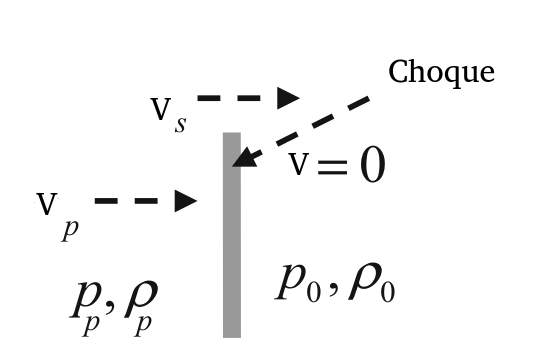
\includegraphics[scale=0.7]{./Figuras/Teoria/move_shock.png}
  \caption{Onda de choque en movimiento sobre un flujo estacionario, tanto la onda como el flujo que está a la izquierda se mueven a la derecha.}\label{fig_move_shock}
\end{figure}
  

Si consideramos nuestro sistema de referencia posicionado sobre la onda (ver Figura \ref{fig:choque:estacionario}), usando las transformaciones de Galileo, las direcciones de las velocidades
se invierten y la velocidad del flujo que entra al choque es $v_s$ y la que sale es $v_s-v_p$.

\begin{figure} 
  \centering
  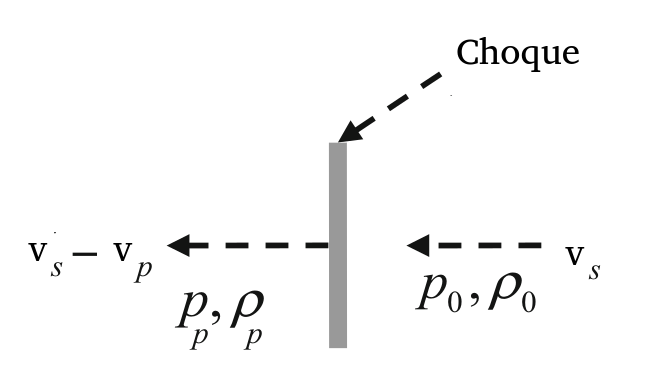
\includegraphics[scale=0.7]{./Figuras/Teoria/stationary_shock.png}
  \caption{Al tomar un sistema de referencia sobre la onda, el choque en movimiento se transforma en una choque estacionario, y los
  flujos que están a la derecha e izquierda de la onda se mueven hacia la izquierda.} \label{fig:choque:estacionario}
\end{figure}

Las ecuaciones de Rankine-Hugoniot parten de las ecuaciones de la hidrodinámica considerando un sistema cerrado usando las ecuaciones \ref{conservación_masa_hidrodinamica}, 
\ref{conservacion_momento_hidrodinamica} y \ref{conservacion_energia_hidrodinamica} donde no varía con el tiempo, es decir, que $\dfrac{\partial}{\partial t}=0$, con lo que se pueden reescribir de la siguiente manera:


\noindent La conservación de masa:
\begin{equation}
  \nabla \cdot \left( \rho \mathbf{u} \right)=0.
\end{equation}

\noindent El momento:
\begin{equation}
  \nabla \cdot \left( \rho \mathbf{u u} \right) + \nabla p = 0.
\end{equation}

\noindent Ecuación de la energía:

\begin{equation}
 \nabla \cdot \left[ \mathbf{u} \left( e+P \right) \right] = 0.
\end{equation}

Considerando una dimensión

\begin{equation}
\dfrac{d \left( \rho u \right)}{d x} = 0,
\end{equation}

\begin{equation}
\dfrac{d \left( \rho u^2 \right)}{d x}+ \dfrac{d p}{d x}=0,
\end{equation}

\begin{equation}
\dfrac{d \left( u\left[e +p \right] \right)}{d x} = 0.
\end{equation}

\noindent Integrando las ecuaciones e igualando a constantes, se pueden reescribir del siguiente modo usando la ecuación de estado $e = \frac{1}{2} \rho u^2 + \frac{p}{\Gamma-1}$ donde 
$e \left[\frac{\mathrm{erg}}{\mathrm{cm^3}}\right]$ 
es la densidad de energía por unidad de volumen

\begin{equation}\label{RH_masa}
\rho_j u_j = \rho_m u_m
\end{equation}

\begin{equation}\label{RH_momento}
\rho_j u_{j}^{2}+p_j = \rho_m u_{m}^{2}+p_m
\end{equation}

\begin{equation}\label{RH_Energia}
\frac{1}{2} u_{j}^{2}+ \frac{\Gamma}{\Gamma-1} \frac{p_{j}}{\rho_{j}} =
 \frac{1}{2} u_{m}^{2}+ \frac{\Gamma}{\Gamma-1} \frac{p_{m}}{\rho_{m}}
\end{equation}

\noindent donde $\rho \left[\frac{\mathrm{g}}{\mathrm{cm}^3}\right]$ representa la densidad, $u \left[\frac{\mathrm{cm}}{\mathrm{s} }\right]$ la velocidad,  $P \left[\frac{\mathrm{dyn}}{\mathrm{cm}^2} \right]$ 
la presión, $\Gamma$ el índice adiabático adimensional donde para velocidades ultrarrelativistas $\Gamma = 4/3$ y para no relativistas $\Gamma = 5/3$ y los índices \textit{j, m} que  relacionan a las propiedades del 
jet y del medio respectivamente. Usando la ecuación   \ref{RH_masa}, se puede definir el flujo como $j \equiv \rho_j u_j = \rho_m u_m$, sustituyendo en la ecuación \ref{RH_momento} se reescribe como:

\begin{equation}\label{RH_momento_j}
p_{j}+\frac{j^2}{\rho_{j}}=p_{m}+\frac{j^2}{\rho_{m}}
\end{equation}

\noindent y la ecuación \ref{RH_Energia} llegamos a:

\begin{equation}\label{RH_Energia_j}
\frac{1}{2} \frac{j^{2}}{\rho_{j}^2}+\frac{\Gamma}{\Gamma-1} \frac{p_{j}}{\rho_{j}}=
\frac{1}{2} \frac{j^{2}}{\rho_{m}^2}+\frac{\Gamma}{\Gamma-1} \frac{p_{m}}{\rho_{m}}.
\end{equation}

\noindent Despejando $j$ de la ecuación \ref{RH_momento_j} obtenemos:
\begin{equation}\label{j^2}
-j^{2}=\frac{p_{j}-p_{m}}{\frac{1}{\rho_{m}}-\frac{1}{\rho_{j}}}.
\end{equation}

\noindent Sustituyendo la ecuación en \ref{j^2} en \ref{RH_Energia_j} obtenemos:

\begin{equation*}
\frac{1}{2} \left( \frac{p_{m}-p_{j}}{\frac{1}{\rho_{j}}-\frac{1}{\rho_{m}}} \right)
\left(\frac{1}{\rho_{j}^{2}}-\frac{1}{\rho_{m}^{2}} \right)
=
\frac{\Gamma}{\Gamma-1}
\left( \frac{p_{m}}{\rho_{m}}-\frac{p_{j}}{\rho_{j}} \right)
\end{equation*}

$\Rightarrow$

\begin{equation*}
\frac{1}{2}	\left( p_{m} - p_{j} \right)
\left( \frac{1}{\rho_{j}}+\frac{1}{\rho_{m}} \right)
=
\frac{\Gamma}{\Gamma-1}
\left( \frac{p_{m}}{\rho_{m}}-\frac{p_{j}}{\rho_{j}} \right)
\end{equation*}

$\Rightarrow$

\begin{equation*}
\frac{1}{\rho_{m}} \left( \frac{1}{2} p_{m}- \frac{1}{2} p_{j}-
\frac{\Gamma}{\Gamma-1} p_{m} \right)
=
\frac{1}{\rho_{j}} \left( \frac{1}{2} p_{j}- \frac{1}{2} p_{m}-
\frac{\Gamma}{\Gamma-1} p_{j} \right)
\end{equation*}

$\Rightarrow$

\begin{equation*}
\frac{1}{\rho_{m}} \left[  \left(\frac{\Gamma + 1}{\Gamma - 1} \right) p_{m} + p_{j} \right]
=
\frac{1}{\rho_{j}} \left[  \left(\frac{\Gamma + 1}{\Gamma - 1} \right) p_{j} + p_{m} \right].
\end{equation*}

\noindent Con lo que queda:

\begin{equation}\label{RH_no_rel_choque_no_fuerte}
\frac{\rho_{m}}{\rho_j} =
\frac{\left( \Gamma +1 \right) p_{m}+ \left( \Gamma -1 \right) p_{j
}}{\left(\Gamma +1 \right) p_{j}+ \left( \Gamma -1 \right) p_{m}}
= \frac{u_j}{u_m}.
\end{equation}

\noindent Si se considera un choque fuerte, es decir, $p_j \gg p_m$, implicaría que $p_m \simeq 0$, por lo que

\begin{equation}
\rho_j = \frac{\Gamma +1}{\Gamma-1} \rho_m 
\end{equation}
Tomando a $\Gamma = 5/3$ da

\begin{equation}
\rho_j = 4 \rho_m,
\end{equation}

\begin{equation}
u_j = \frac{1}{4} u_m,
\end{equation}

\begin{equation}
p_{j} = \frac{3}{4}\rho_m u_m^{2}.
\end{equation}




\subsection{Condiciones de Taub}



Como se menciona en \citet{Landau1987} si se considera la conservación de masa:

\begin{equation}
  \rho_j v_j \gamma_j=  \rho_{\infty} v_{\infty} \gamma_{\infty}
\end{equation}

\noindent donde $v_j$, $v_\infty$ es la velocidad del jet y del medio que lo rodea respectivamente. Despejando $\rho_{\infty}$ se obtiene:

\begin{equation}\label{eq_masa_densidad_despejada}
  \rho_\infty = \rho_j \frac{v_j \gamma_j }{v_\infty \gamma_\infty}.
\end{equation}

\noindent Tambien se considera la ecuación de momentos

\begin{equation}
  \left( e_j + p_j\right) v^2_j \gamma^2_j + p_j = \left( e_{\infty} + p_{\infty}\right) v^2_{\infty} \gamma^2_{\infty} + p_{\infty}.
\end{equation}

\noindent La densidad de energía se compone de la energía interna del sistema y de la energía cinética

\begin{equation} \label{eq_densidad_de_energia}
  e = e_{int} + e_k.
\end{equation}

\noindent La energía interna para un sistema ultra-relativista es $ p = \frac{1}{3}e_{int}$ lo que implica que $e_{int} = 3p$, mientras que la densidad de energía
cinética es $e_k = \rho c^2$, pero como se esta considerando a $c = 1$ esto se reduce a $e_k = \rho$. Sustituyendo todo esto en la ecuación
\ref{eq_densidad_de_energia} queda:

\begin{equation} \label{eq_momentos_relativista_modificada}
  \left( \rho_j + 4p_j \right) v^2_j \gamma^2_j  +p_j = \left( \rho_\infty + 4p_\infty \right) v^2_{\infty} \gamma^2_{\infty}  +p_\infty.
\end{equation}

\noindent Con la ecuación \ref{eq_masa_densidad_despejada} podemos modificar la ecuación \ref{eq_momentos_relativista_modificada}, con lo que queda:

\begin{equation}
  \left( \rho_j + 4p_j \right)v_j \gamma^2 +p_j = \left( \rho_\infty + 4p_\infty \right)v_\infty \gamma^2 +p_\infty
\end{equation}

\noindent y tomando un choque fuerte $p_j \gg p_\infty $ podemos reducir la ecuación a 

\begin{equation} \label{eq_momentos_choque_fuerte}
  \left( \rho_j + 4p_j \right)v_j^2 \gamma^2 +p_j =  \rho_\infty  v_\infty^2 \gamma_{\infty}^{2}. 
\end{equation}

\noindent Sustituyendo la ecuación \ref{eq_masa_densidad_despejada} en \ref{eq_momentos_choque_fuerte} obtenemos:

\begin{equation}
  \left( \rho_j + 4p_j \right)v_j^2 \gamma^2 +p_j = \rho_j v_j v_\infty \gamma_j \gamma_\infty.
\end{equation}

\noindent Suponiendo $\left( \rho_j + 4p_j \right)v_j^2 \gamma^2 \gg p_j $



\begin{equation}
  \left( \rho_j + 4p_j \right)v_j \gamma_j = \rho_\infty v_\infty  \gamma_\infty.
\end{equation}

\noindent Despejando la presión obtenemos

\begin{equation}
  p_j = \frac{\rho_j}{4}\left(\frac{v_\infty}{v_j} \frac{\gamma_\infty}{\gamma_j}-1\right),
\end{equation}

\noindent como $v_j \thickapprox v_\infty \thickapprox c$

\begin{equation}
  p_j = \frac{\rho_j}{4}\left( \frac{\gamma_\infty}{\gamma_j}-1\right).
\end{equation}

Para poder simular las condiciones de un jet, se necesita saber la densidad, velocidad y presión del mismo, como los jet tienen velocidades cercanas a la
de la luz, se pueden tomar valores cercanos a esta constante. La densidad se obtendrá en la siguiente sección. 


\subsection{Luminosidad}
Si suponemos las condiciones de Taub en un jet relativista y si colocamos nuestro marco de referencia sobre el jet, la energía será:

\begin{equation} \label{eq._energia_relativista}
  E = \gamma_{\infty} M c^2
\end{equation}

\noindent donde $\gamma_{\infty}$ es factor de Lorentz con el que se mueve el jet cuando ya se ha alejado del objeto compacto y como sabemos 
que $L \equiv \dfrac{d E}{d t}$ entonces derivando la ecuación \ref{eq._energia_relativista} respecto al tiempo tenemos:

\begin{equation} \label{eq._luminosidad_relativista}
  \dfrac{d E}{d t} = \gamma_{j} \dot{ M }  c^2.
\end{equation}

La taza de flujo de masa $\dot{M}$ se puede escribir como:

\begin{equation}
  \dot{M} = \rho_j u_j A_j
\end{equation}

\noindent donde $\rho$ es la densidad, $u_j = v_j \gamma_{j}$ es la cuadrivelocidad,  y $A_j$ es el área, que en este caso, corresponde la parte esférica del jet, entonces la luminosidad se puede escribir como:

\begin{equation}
  L \equiv \dfrac{d E}{d t} = 4\pi r_j^2 \rho_j v_j \gamma_j \gamma_{\infty} c^2,
\end{equation}

\noindent despejando la densidad

\begin{equation}
  \rho = \frac{L}{4\pi r_j^2 v_j \gamma_j \gamma_{\infty} c^2}
\end{equation}

% Al obtener la densidad ya podemos simular el jet dado que la luminosidad se puede obtener de detectores de Rayos $\gamma$ y las velocidades también ? preguntar a 
% Diego


\section{Solución de Sedov-Taylor} \label{sec:sedov_taylor}

%Ojo Julio
Una forma de verificar si el código funciona correctamente es ver si una onda de choque esférica (o circular en 2D) sigue la solución analítica y auto similar obtenida por Sedov y Taylor (véase \citet{PAFD}). 
Cabe señalar que la onda de choque esférica es descrita por la inyección de energía dentro de un radio, el cual está inmerso en un medio en reposo. 

\subsection{Aproximación en función del análisis dimensional}
Si se considera un choque fuerte,
es decir, $p_w \gg p_m$,
entonces las únicas variables que se pueden tomar son $E$, $\rho_w$ y $t$ que es el tiempo.
Las dimensiones de estas cantidades se muestran a continuación. 

\begin{equation}
  \left[ \rho_w \right] = \frac{M}{L^3},
\end{equation}

\begin{equation}
  \left[E\right] = M \frac{L^2}{T^2},
\end{equation}

\begin{equation}
  \left[ t\right] = T.
\end{equation}

\noindent La única cantidad que se puede construir que contenga la energía, tiempo y la densidad y que su dimensión sea la longitud es:

\begin{equation}
  \left[ \left( \frac{Et^2}{ \rho_w } \right)^{\frac{1}{5}}\right] = L,
\end{equation}

\noindent por lo que para cualquier radio de onda de cualquier choque, debe depender de estas variables

\begin{equation}
  R(t) = \eta  \left( \frac{Et^2}{ \rho_w } \right)^{\frac{1}{5}} \varpropto t^{\frac{2}{5}}.
\end{equation}

\noindent Por lo que la constante $\eta$ debe ser de la siguiente manera

\begin{equation}
  \eta \equiv \frac{r}{\left( \frac{Et^2}{\rho_w} \right)^{\frac{1}{5}}}.
\end{equation}



\subsection{Aproximación en función de la conservación de la energía}

Otra aproximación es buscando el cociente de presiones y densidades en función del número Mach.
Se puede saber el radio $R(t)$ de una onda de choque en función del tiempo. Tomando el volumen de una esfera es $V = \frac{4}{3} \pi * R^3$ y la densidad de la región interior al choque es constante, entonces 
el volumen $V = \frac{M}{\rho_w}$. La velocidad media de la onda es $v(t) \sim \frac{R(t)}{t} $
por lo que se puede aproximar la energía cinética de la onda como 

\begin{equation}
	E_{kin} \sim \frac{1}{2} M v^2 \sim \rho_w R^3 \left( \frac{R}{t} \right) ^2 = \rho_w \frac{R^5}{t^2}.
\end{equation}

\noindent La energía térmica de un gas ideal (monoatómico) es 

\begin{equation} \label{eq_energia_termica}
	E_{th} \sim \frac{3}{2}pV.
\end{equation}

\noindent Para encontrar la presión, primero se definirán algunas ecuaciones. La entalpía de estancamiento se define en términos de la entalpía y la velocidad de la onda 

\begin{equation}
	h_0 = h + \frac{1}{2} v^2
\end{equation}

\noindent la cual la podemos reescribir como

\begin{equation} \label{eq_entalpía}
	h_0 = h + \left( 1 +\frac{1}{2} \frac{v^2}{h} \right).
\end{equation}

\noindent La velocidad del sonido puede ser definida como 

\begin{equation} \label{eq_sonido_1}
	a = \sqrt{\frac{\Gamma p}{\rho}}
\end{equation}

\noindent y también como 

\begin{equation} \label{eq_sonido_2}
	a = \sqrt{(\Gamma-1) h}
\end{equation}

\noindent donde $a$ es la velocidad del sonido, $h$ la entalpía, $v$ la velocidad, $p$ la presión y $\rho$ la densidad. También se define el número de Mach 

\begin{equation} \label{eq_Mach}
	M = \frac{v}{a}
\end{equation}

Si se combina la ecuación \ref{eq_sonido_1} con la ecuación \ref{eq_Mach} y lo sustituimos en la ecuación \ref{eq_entalpía} se obtiene la entalpía en función de la velocidad de la onda y del sonido

\begin{equation} \label{h_0_función_aire_mach}
	h_0 = \frac{a^2}{\Gamma - 1} \left( 1 + \frac{\Gamma - 1}{2} M^2 \right).
\end{equation}

\noindent Esta ecuación servirá más adelante. Usando las ecuaciones  
\ref{RH_Energia} y \ref{entalpía_función_presion_densidad} para obtener la ecuación de la energía en función de la entalpía, va a quedar como:

\begin{equation}\label{RH_entalpía}
  h_w +\frac{1}{2}v_w^2 = h_m +\frac{1}{2}v_m^2
\end{equation} 

\noindent donde los subíndices $w$, $m$ corresponden a la onda y al medio respectivamente. Dividiendo la ecuación \ref{RH_momento} entre \ref{RH_masa}, y cambiando los 
subíndices $j$ por $w$ se obtiene la siguiente ecuación: 

\begin{equation} \label{RH_momento_masa}
  v_w + \frac{p_w}{\rho_w v_w} = v_m + \frac{p_m}{\rho_m v_m}
\end{equation}

\noindent Usando la ecuación \ref{eq_sonido_1} en la ecuación \ref{RH_momento_masa} se puede reescribir de 
la siguiente manera:

\begin{equation} \label{eq_diferencia_velocidades}
  v_w-v_m = \frac{1}{\Gamma} \left(\frac{a_m^2}{v_m} - \frac{a_w^2}{v_w} \right).
\end{equation}

Se puede usar la entalpía de estancamiento para llegar a la siguiente igualdad:

\begin{equation}
  h_w + \frac{1}{2} v_w = h_m + \frac{1}{2} v_m \equiv h_0,
\end{equation}

\noindent definiendo a la velocidad del sonido como:

\begin{equation} \label{eq_sonido_onda}
  a_w^2 = \left( \Gamma-1 \right) h_w = \left( \Gamma-1 \right) \left( h_0 -\frac{1}{2} v_w^2 \right)
\end{equation}

\begin{equation} \label{eq_sonido_medio}
  a_m^2 = \left( \Gamma-1 \right) h_m = \left( \Gamma-1 \right) \left( h_0 -\frac{1}{2} v_m^2 \right)
\end{equation}

\noindent sustituyendo las ecuaciones \ref{eq_sonido_onda} y \ref{eq_sonido_medio} en la ecuación \ref{eq_diferencia_velocidades}
se obtiene

\begin{equation}
  v_w-v_m = \frac{\Gamma - 1}{\Gamma} h_0 \left[ \frac{1}{v_m} - \frac{1}{u_w} + \frac{1}{2} \left( v_w - v_m\right) \right]
\end{equation}

\noindent dividiendo por $ \left( v_w - v_m \right)$

\begin{equation}
  1 = \frac{\Gamma - 1}{\Gamma} \left( \frac{h_0}{v_m v_w} + \frac{1}{2} \right),
\end{equation}

\noindent que al final se puede reescribir como:

\begin{equation} \label{eq_denominador}
  \frac{1}{v_w v_m} = \frac{1}{\left( \Gamma -1\right) h_0} \frac{\Gamma + 1}{2}
\end{equation}

Otra ecuación de utilidad es la definición de Mach, ya que

\begin{equation}\label{velocidad_aire_mach}
  v_w^2 = a_w^2 M_w^2.
\end{equation}

\noindent Entonces usando la ecuacion \ref{h_0_función_aire_mach}, se puede reescribir la ecuación \ref{velocidad_aire_mach}
como:

\begin{equation} \label{eq_numerador}
  v_w^2 = M_w^2 \frac{\left( \Gamma -1 \right) h_0}{1+\frac{\Gamma - 1}{2} M_w^2}.
\end{equation}

\noindent Usando la ecuación de momentos \ref{RH_masa}, se puede reescribir de la siguiente manera:

\begin{equation} \label{eq_fraccion_momentos}
  \frac{\rho_m }{\rho_w} = \frac{ v_w}{v_m} = \frac{v_w^2}{v_w v_m}.
\end{equation}

Como ya se sabe cuanto vale el numerador (ec. \ref{eq_numerador}) y el denominador (ec. \ref{eq_denominador})
de la fracción, entonces se puede definir el cociente de las densidades \ref{eq_fraccion_momentos} como:

\begin{equation}\label{eq_fraccion_momentos_funcion_mach}
  \frac{\rho_m}{\rho_w} = \frac{\left( \Gamma +1 \right) M_w^2}{2+ \left( \Gamma -1 \right) M_w^2}.
\end{equation}

\noindent Entonces para encontrar las presiones, se pueden combinar las ecuaciones \ref{RH_momento} y \ref{RH_masa} 

\begin{equation}
  p_m - p_w = \rho_w v_w^2 - \rho_m v_m^2 = \rho_w v_w^2 \left( 1 - \frac{v_m}{v_w}\right) = \rho_w v_w^2 \left( 1 - \frac{\rho_w}{\rho_m}\right).
\end{equation}

\noindent Empleando la siguiente relación $\rho v^2 = \Gamma p M^2$, que se obtiene de las ecuaciones \ref{eq_sonido_1} y
\ref{eq_Mach}, dividiendo por $p_w$ y sustituyendo  $\frac{\rho_m}{\rho_w}$ de la ecuación 
\ref{eq_fraccion_momentos_funcion_mach} queda:

\begin{equation} \label{eq_fraccion_Presiones}
  \frac{p_m}{p_w} = 1 + \frac{2 \Gamma}{\Gamma + 1} \left( M_w^2 -1\right).
\end{equation}

\noindent Si se usa la siguiente relación $ p_w = \frac{\rho a_w^2 }{\Gamma}$ se puede obtener el límite del choque fuerte

\begin{equation}
  p_m  \simeq \frac{2 \rho_w v_w^2}{\Gamma + 1}.
\end{equation}

\noindent Con esto ya se puede obtener la energía térmica de la ecuación \ref{eq_energia_termica} por lo que queda: 

\begin{equation}
  E_{th} \sim P R^3 \sim \rho v^2 R^3 \sim \rho \frac{R^5}{t^2}.
\end{equation}

\noindent Dado que tienen el mismo orden que el de la energía cinética, entonces la energía total que es una cantidad conservada, se puede esperar que:

\begin{equation}
  E_t = E_{kin} + E_{th} \sim \rho \frac{R^5}{t^2}
\end{equation}

\noindent Despejando el radio, obtenemos lo siguiente

\begin{equation} \label{eq_Radio_proporcional}
  R(t) \varpropto \left(\frac{E t^2}{\rho_w}\right)^{\frac{1}{5}}.
\end{equation}

\noindent En la Figura \ref{fig_Radio_v_tiempo} se observa una función parecida a la logaritmica. Su radio de expansión no crece muy rápidamente conforme avanza el tiempo.

\begin{figure}
  \centering
    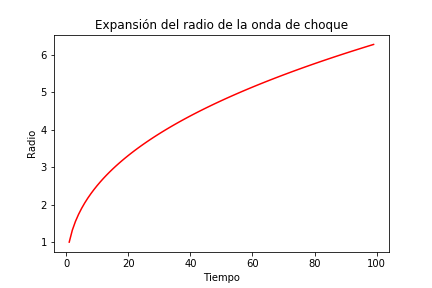
\includegraphics[width=0.5\textwidth]{Figuras/Teoria/Radio_vs_tiempo.png}
  \caption{Radio de expansión de una onda de choque conforme avanza el tiempo. } \label{fig_Radio_v_tiempo}
\end{figure}

Derivando la ecuación \ref{eq_Radio_proporcional}, se obtiene la velocidad

\begin{equation}
  \dfrac{de}{dt} = \frac{2}{5}\frac{R(t)}{t} \varpropto t^{\frac{-3}{5}}.
\end{equation}

\noindent A diferencia del radio, la velocidad, se asemeja más a una asíntota que decrece muy rápidamente (veáse la Figura \ref{fig_velocidad_vs_radio}).

\begin{figure}
  \centering
    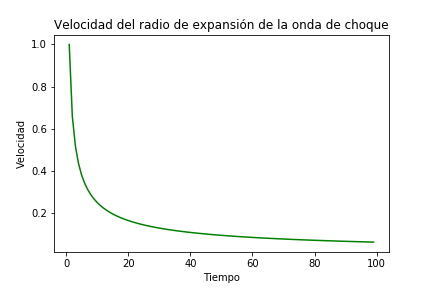
\includegraphics[width=0.5\textwidth]{Figuras/Teoria/Velocidad_vs_tiempo.png}
  \caption{Velocidad del radio de expansión de una onda de choque conforme avanza el tiempo. } \label{fig_velocidad_vs_radio}
\end{figure}



% ======================================NUEVO CAPITULO ================================================
% ======================================NUEVO CAPITULO ================================================
% ======================================NUEVO CAPITULO ================================================
% ======================================NUEVO CAPITULO ================================================

\chapter{Verificación del código}\label{cap:Verificacion_del_codigo}


\section{Pruebas unidimensionales}

Para tener la seguridad de que el código hidrodinámico funcione bien se realizaron pruebas  unidimensionales (1D)
de un tubo de Sod ya sea en el régimen newtoniano así como en el relativista (en ambos regímenes se usó
el método de Lax así como el HLL, y se compararon los resultados con la solución analítica). 
Estas pruebas consisten en determinar cómo se comporta un gas ideal en un tubo 1D 
el cual se tiene inicialmente una discontinuidad. Esto es, que en un valor determinado,
el gas cambia abruptamente los valores de la densidad, presión y velocidad.




\subsection{Casos newtonianos} \label{subsec:casos_newtonianos_1D}

Los valores de $\rho$, $p$ y $v$ de los modelos newtonianos se indican en el cuadro
\ref{Cuadro_parametros_sod_tube}. El primer  modelo (denominado caso 1 newtoniano), produce una onda 
de rarefacción\footnote{
  Una onda de rarefacción es la progresión de partículas que se aceleran lejos de una zona 
  comprimida. Siempre se mueven a regiones de mayor densidad y no presentan discontinuidades.
} que se mueve a la izquierda y una onda de choque\footnote{
  Una onda de choque se moverá siempre a las zonas de menor densidad y presentará discontinuidades, además
  de que su valor siempre será una constante.
} que se mueve a la derecha. La condición inicial\footnote{
  Dado que para el primer caso tendremos valores de densidad
  y presión más grandes que el lado derecho de la posición crítica ($x_0$), 
  podemos decir que del lado izquierdo 
  de $x_0$ será una onda de rarefacción que se moverá a la izquierda, mientras que del lado
  derecho será una onda de choque que se moverá a la derecha.
} del gas consiste en tener el dominio 
unidimensional dividido en un lugar del dominio (en $x_0$) con ciertos valores de densidad ($\rho_l$), 
velocidad ($v_l$) y presión ($p_l$) del lado izquierdo\footnote{Los subíndices \emph{l} y \emph{r} 
vienen del inglés \emph{left} y \emph{right} que significan izquierda y derecha respectivamente.}, 
mientras que del lado derecho tendrán densidad ($\rho_r$), velocidad ($v_r$) y  presión ($p_r$). 
La elección del índice adiabático $\Gamma = 7/5$, un dominio $x \in [0,1]$ cm y $x_0 = 0.5$ cm 
se dió para poder simular y comparar los mismos modelos
mostrados por \citet{Lora2013}.

\begin{table}[htbp]
  \begin{center}
  \begin{tabular}{|c|c|c|c|c|c|c|}
  \hline 
  \textbf{Caso} & \textbf{$p_l$} [$\text{dyn}/\text{cm}^2$] & \textbf{$p_r$} [$\text{dyn}/\text{cm}^2$]& \textbf{$v_l$} [$\text{cm}/\text{s}$]& \textbf{$v_r$} [$\text{cm}/\text{s}$]& \textbf{$\rho_l$} [$\text{g}/\text{cm}^3$]& \textbf{$\rho_r$} [$\text{g}/\text{cm}^3$] \\ 
  \hline 
  Caso 1 & 1.0  & 0.1  & 0.0 & 0.0 & 1.0  & 0.125 \\ 
  \hline 
  Caso 2 & 0.4  & 0.4  & -1.0 & 1.0 & 1.0  & 1.0  \\ 
  \hline 
  \end{tabular}
  \caption{\label{Cuadro_parametros_sod_tube} Valores iniciales de la presión ($p$), velocidad ($v$)
  y densidad ($\rho$), del lado izquierdo ($p_l, v_l, \rho_l$) y derecho ($p_r, v_r, \rho_r$)
  para los casos newtonianos. Para todos los
  casos el dominio espacial es $x \in [0,1]$ cm, la posición crítica sería
  $x_0 = 0.5$ cm y un índice adiabático $\Gamma = 7/5$.}
  \end{center}
\end{table}


En la Figura \ref{caso_new_rar_shock} se muestra la evolución temporal en tres 
tiempos característicos $t = 0, \, 0.2, \, 0.4$
de la densidad, 
presión y velocidad para el caso 1 newtoniano usando el método Lax. En la Figura se ve como 
una onda de choque viaja hacia la derecha a través de la región de baja densidad.
En el panel superior izquierdo
notamos como para 0.2 segundos el perfil de densidad $\rho$ tiene dos brincos situados 
aproximadamente en 
$x \approx 0.70$ cm, donde la densidad ($\rho \approx 0.48 \,  \text{g}/ \text{cm}^3$), 
cambia a $\rho \approx 0.28 \,  \text{g}/ \text{cm}^3$, mientras la velocidad y la presión 
mantienen los mismos valores 
($v \approx 0.99$ cm/s y $p \approx 0.3 \,  \text{dyn}/ \text{cm}^2 $).
En x=0.85 cm, la velocidad ($v \approx 0.99$ cm/s), presión 
($p \approx 0.3  \,  \text{dyn}/ \text{cm}^2 $)  y  densidad 
($\rho \approx 0.28 \,  \text{g}/ \text{cm}^3$) 
tienen una discontinuidad y cambian sus valores a los valores iniciales del estado derecho del tubo
que no han sido afectados por la onda. 
La primera discontinuidad hace referencia a la onda de contacto que tiene la misma velocidad
que los estados de la izquierda y la derecha $V_c = v_l = v_r$ donde $V_c$
es la velocidad de la onda de contacto, por lo que esto hace que las presiones sean iguales 
$p_l = p_r$. Esta primera discontinuidad solo se 
presenta en el panel de las densidades, la otra discontinuidad que se presenta en los 3 paneles es la 
discontinuidad de la onda de choque.
Para el tiempo t=0.4 s
la discontinuidad de la onda de choque ya no se presenta en nuestro dominio de los 3 paneles, mientras 
que la cabeza de la onda de rarefacción todavía se muestra en $x \approx 0.01$ cm. La única discontinuidad 
presente es la de onda de 
contacto, donde $\rho$ cambia su valor de $\rho \approx 0.48 \,  \text{g}/ \text{cm}^3$
a $\rho \approx 0.28 \,  \text{g}/ \text{cm}^3$, mientras la velocidad $v \approx 0.99$ cm/s y 
presión $p \approx 0.3 \,  \text{dyn}/ \text{cm}^2 $ mantienen
sus mismos valores.
% Esta onda es más lenta que la de rarefacción ya que se encuentra en $x \approx 0.85$ cm.

  \begin{figure}
    \centering
        \subfigure{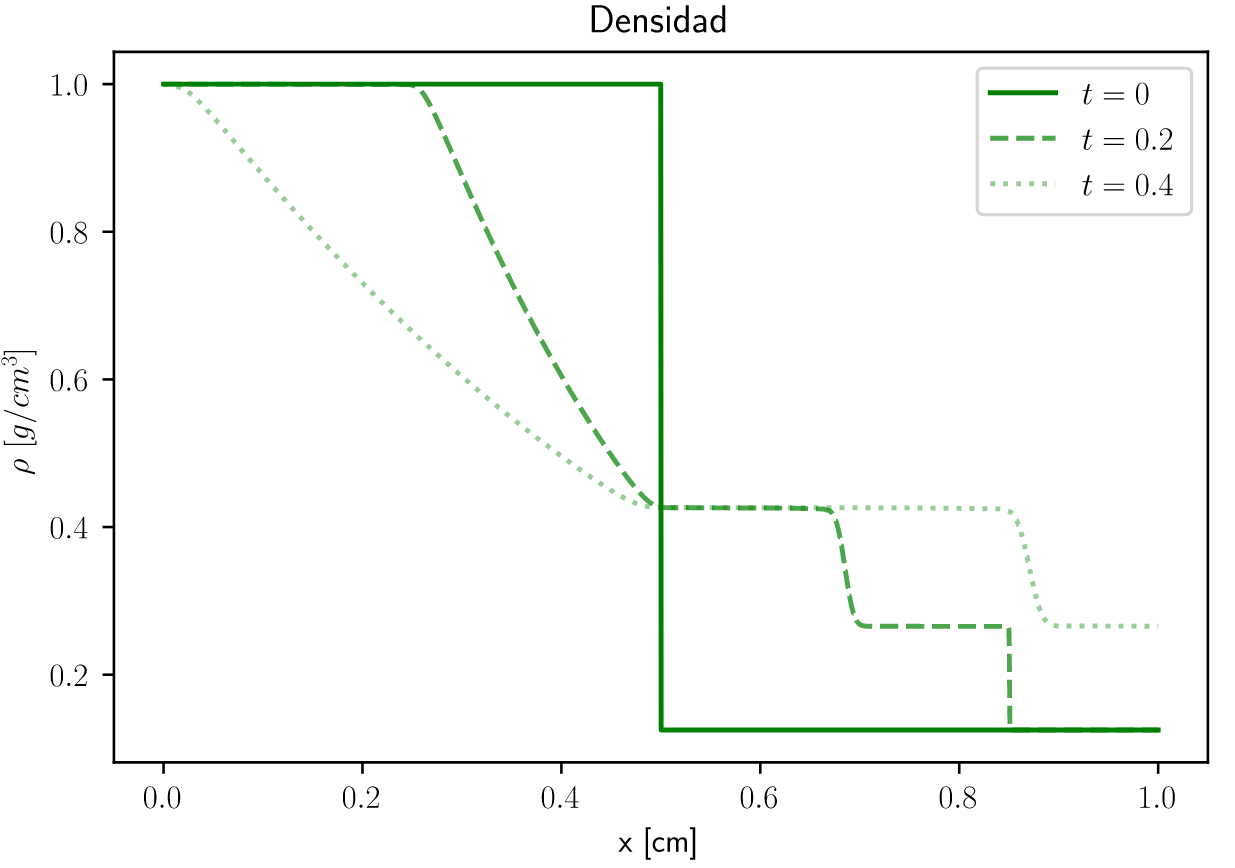
\includegraphics[scale = 0.16]{./Figuras/verificacion_del_codigo/caso_newtoniano/caso_new_rar_shock_rho.png}}
        \subfigure{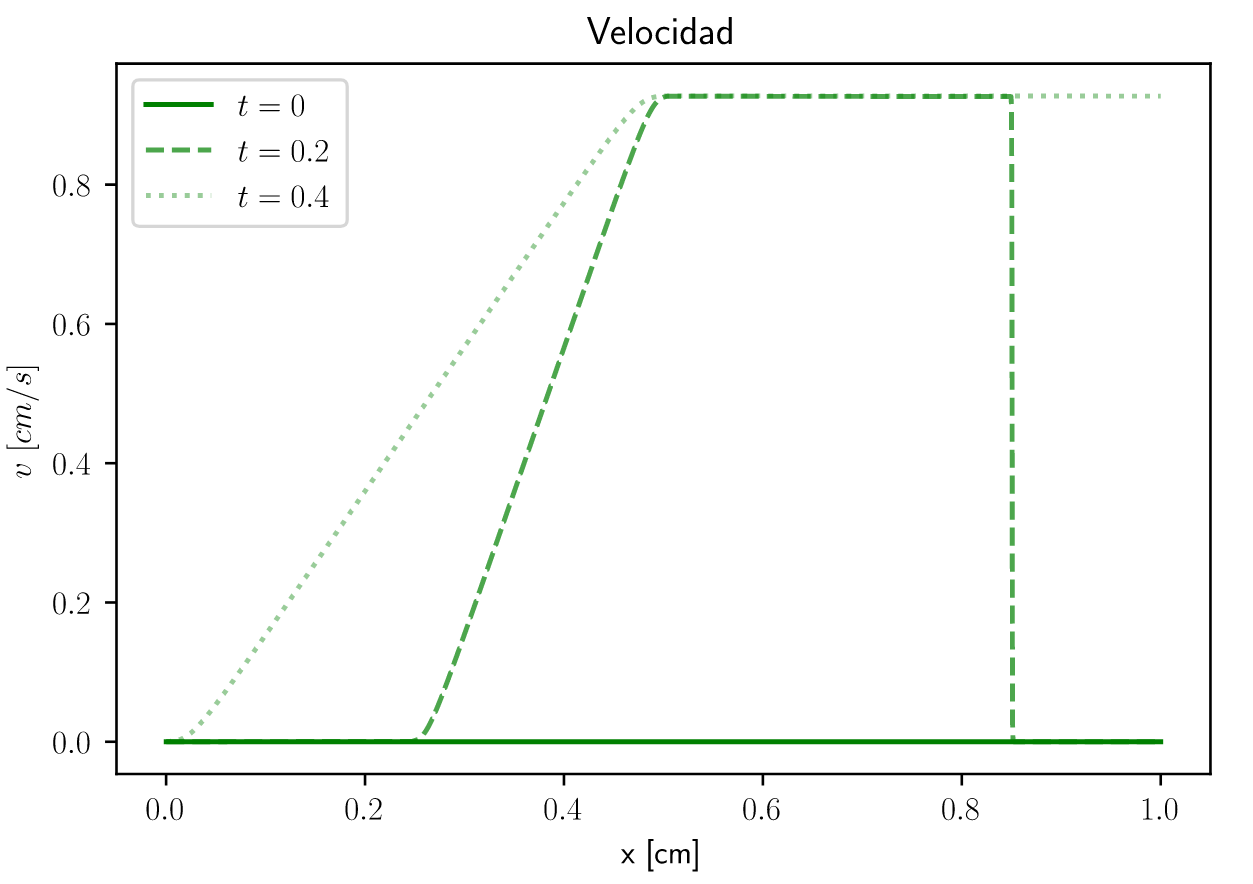
\includegraphics[scale = 0.16]{./Figuras/verificacion_del_codigo/caso_newtoniano/caso_new_rar_shock_v.png}}
        \subfigure{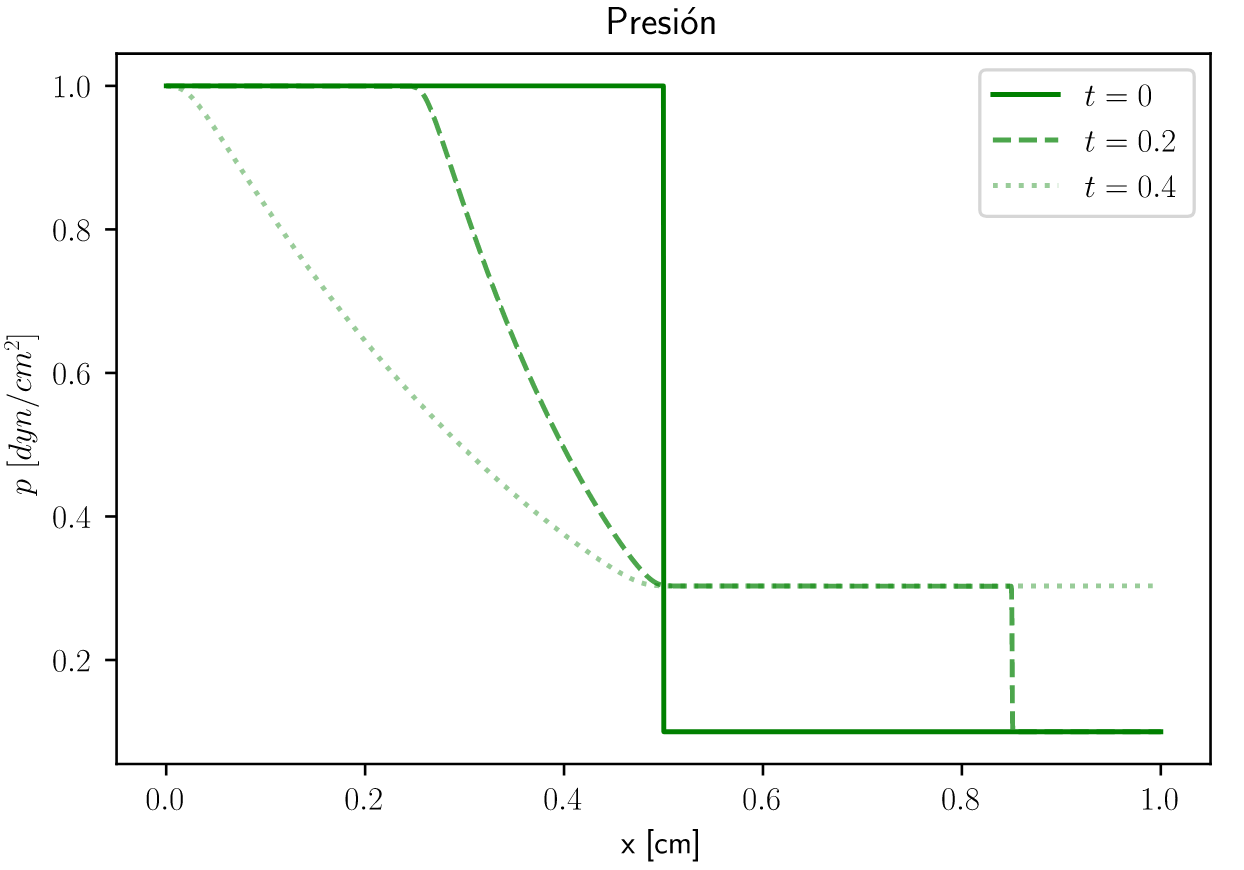
\includegraphics[scale = 0.16]{./Figuras/verificacion_del_codigo/caso_newtoniano/caso_new_rar_shock_p.png}}
      \caption{\label{caso_new_rar_shock} Evolución temporal del caso 1 newtoniano (usando el método Lax) donde se muestra
      las magnitudes de densidad (arriba a la izquierda), presión (abajo) y 
      velocidad (arriba a la derecha). 
      Se usó un índice adiabático $\Gamma = 7/5$ .}
  \end{figure}

  El caso 1 newtoniano también fue resuelto utilizando el método HLL y usando varias resoluciones. 
  En la Figura 
  \ref{comparacion_analitico_newtoniano_caso_1}, se muestra la comparación de la $\rho, \, v$ y $p$
  entre los métodos Lax 
  y HLL a 10,000 píxeles. 
  El panel de arriba a la izquierda muestra la densidad $\rho = 1.0 \,  \text{g}/ \text{cm}^3$ 
  donde presenta un cambio en 
  $x \approx 0.24 $ cm y baja gradualmente hasta $x \approx 0.48$ cm donde la densidad ahora es $\rho \approx
  0.45 \,  \text{g}/ \text{cm}^3$. Se puede ver que tanto Lax y HLL tienen el 
  mismo comportamiento
  que el método analítico. 
  Para las discontinuidades en $x \approx 0.74$ cm (contacto) y $x \approx 0.93$ cm (choque) cambian los valores de densidad $
  \rho \approx 0.48 \,  \text{g}/ \text{cm}^3$ a $\rho \approx 0.35 \,  \text{g}/ \text{cm}^3$ respectivamente y 
  después a $\rho =0.1 \,  \text{g}/ \text{cm}^3$. 
  Se puede observar que
  tanto Lax como HLL presentan dificultad con la discontinuidad de contacto, 
  pero logra adaptarse muy bien para la discontinuidad de choque. En sí, ambos métodos reproducen 
  casi a 
  la perfección toda la región donde se desarrolla la discontinuidad en resoluciones de 10,000 píxeles.
  En el panel de arriba a la derecha se muestra como tanto HLL como Lax también reproducen la 
  solución analítica esperada para
  la velocidad. Esta, al igual que la densidad, cambian 
  sus valores gradualmente de $v = 0$ cm/s en $x \approx 0.20$ cm a $v \approx 0.99$ cm/s en 
  $x \approx 0.50$ cm,
  donde se mantiene constante hasta la discontinuidad de choque en $x \approx 0.93$ cm y regresa a $v = 0$ cm/s.
  En este punto, tanto Lax como HLL, no tiene ninguna dificultad al reproducir la discontinuidad de 
  choque.
  El panel de abajo a la izquierda muestra como HLL y Lax reproducen la solución 
  analítica para
  la presión, la cual cambia su valor 
  $p = 1.0 \,  \text{dyn}/ \text{cm}^2 $ en $x \approx 0.48$ cm
  bajando hasta $p \approx 0.3 \,  \text{dyn}/ \text{cm}^2 $ en $x \approx 0.48$ cm, 
  donde igual que la velocidad
  mantiene su mismo valor hasta $x \approx 0.93$ cm donde su valor decae a $p = 0.1 \,  \text{dyn}/ \text{cm}^2 $.



El panel de abajo a la derecha de la Figura 
\ref{comparacion_analitico_newtoniano_caso_1} muestra cómo varían los resultados
usando Lax con distintas resoluciones ($n_x = 10^2, \, 10^3, \,10^4$), además, se muestra la solución
analítica.
Queda claro cómo 
conforme se incrementa la resolución (píxeles\footnote{Para fines prácticos, usaremos la palabra "píxel" para describir las celdas con tamaño $\Delta x$ en 
las que se divide nuestro dominio espacial, es decir, si el dominio tiene una resolución de $n$ 
píxeles, entonces, $\Delta x = 1/n$ }) los resultados numéricos se apegan más a la analítica. 
En específico, para el problema 1 newtoniano, a partir de resoluciones mayores a 1000 píxeles,
los resultados 
se apegan mucho a la solución analítica.

\begin{figure}
  \centering
    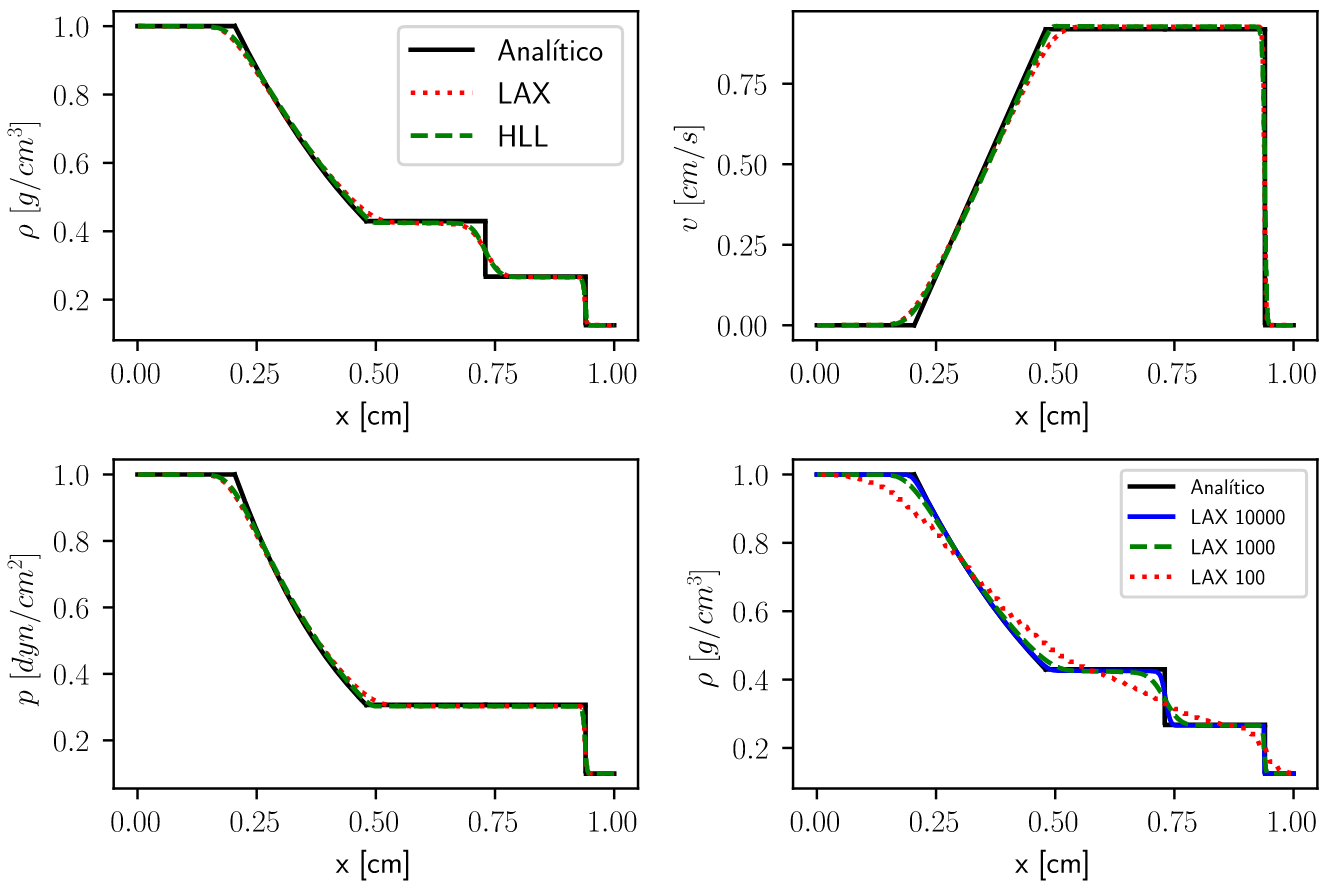
\includegraphics[width=1.0\textwidth]{./Figuras/verificacion_del_codigo/rarefaction.png}
  \caption{Representación del caso 1 newtoniano a $t = 0.25$ s. Las magnitudes mostradas con
  la densidad (arriba a la izquierda), la velocidad (arriba a la derecha) y la presión (abajo a la 
  izquierda).
  El panel de abajo hacia la derecha muestra la comparación a distintas resoluciones para la densidad. Los demás paneles muestran
  las diferencias de los métodos HLL y Lax con una resolución de 10,000 píxeles.
  \label{comparacion_analitico_newtoniano_caso_1}}
\end{figure}

En el 2º caso newtoniano, los valores de la densidad y presión fueron las mismas en ambos estados del tubo, pero las velocidades fueron de igual magnitud
pero de sentido contrario. Esta condición inicial produce 2 ondas de rarefacción. Una se mueve hacia
la izquierda y la otra hacia la derecha (véase el cuadro \ref{Cuadro_parametros_sod_tube} para más
detalles).
La Figura \ref{caso_new_rar_rar} muestra, usando
el método de Lax, la evolución temporal del 2° caso newtoniano. El panel de arriba a la izquierda muestra la densidad.
El panel arriba a la derecha muestra la velocidad y el de abajo la presión. En todos los paneles se 
muestra $t = 0 \, , t = 0.2 \, ,t = 0.4$.

\begin{figure}
  \centering
      \subfigure{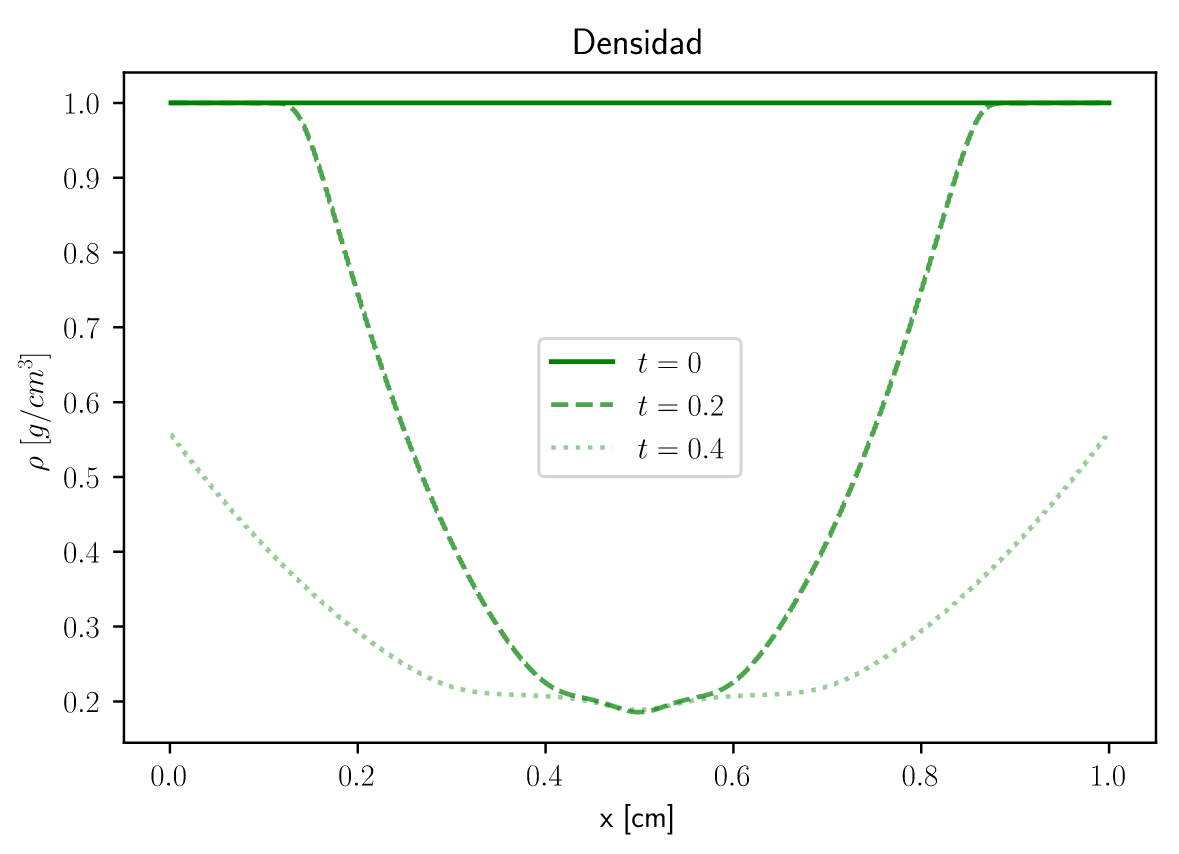
\includegraphics[scale = 0.16]{./Figuras/verificacion_del_codigo/caso_newtoniano/caso_new_rar_rar_rho.png}}
      \subfigure{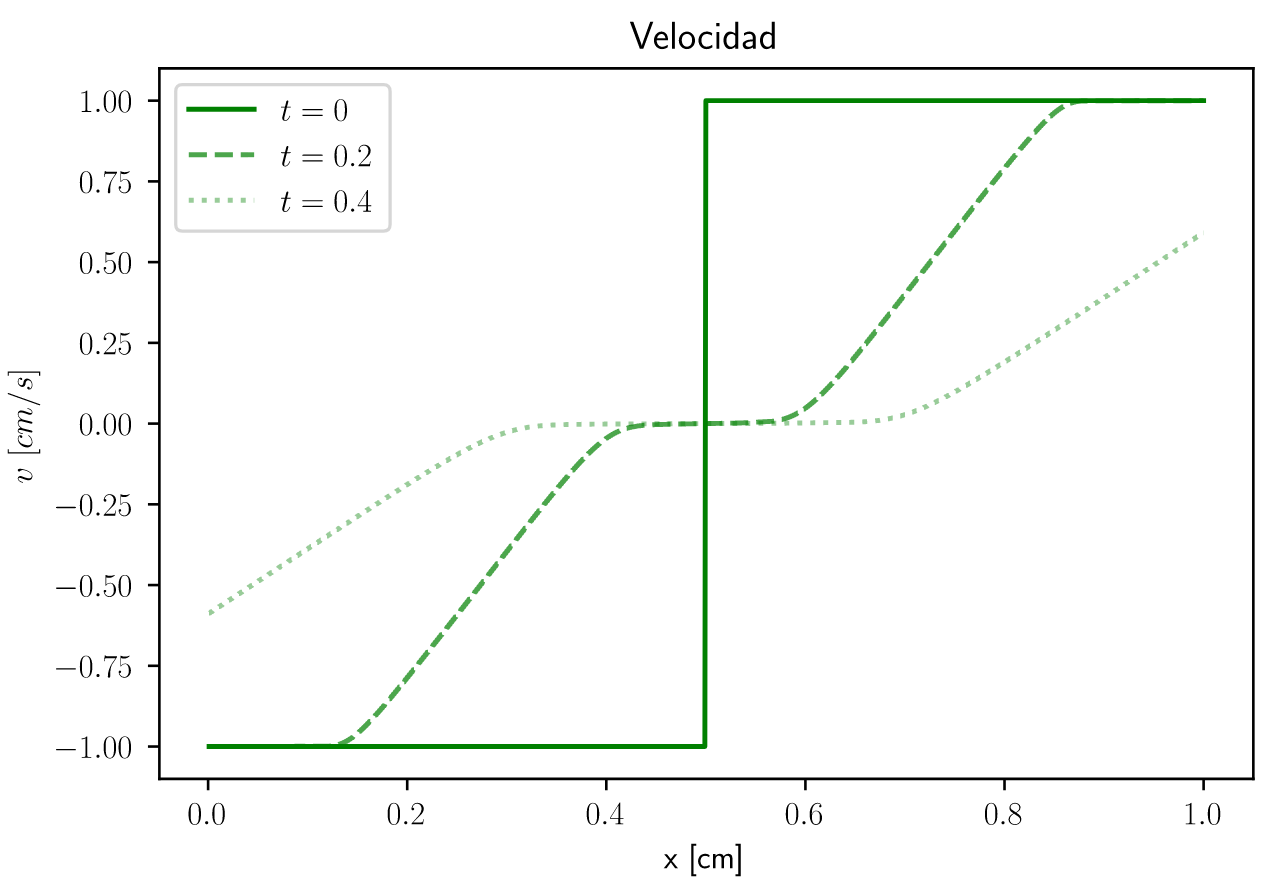
\includegraphics[scale = 0.16]{./Figuras/verificacion_del_codigo/caso_newtoniano/caso_new_rar_rar_v.png}}
      \subfigure{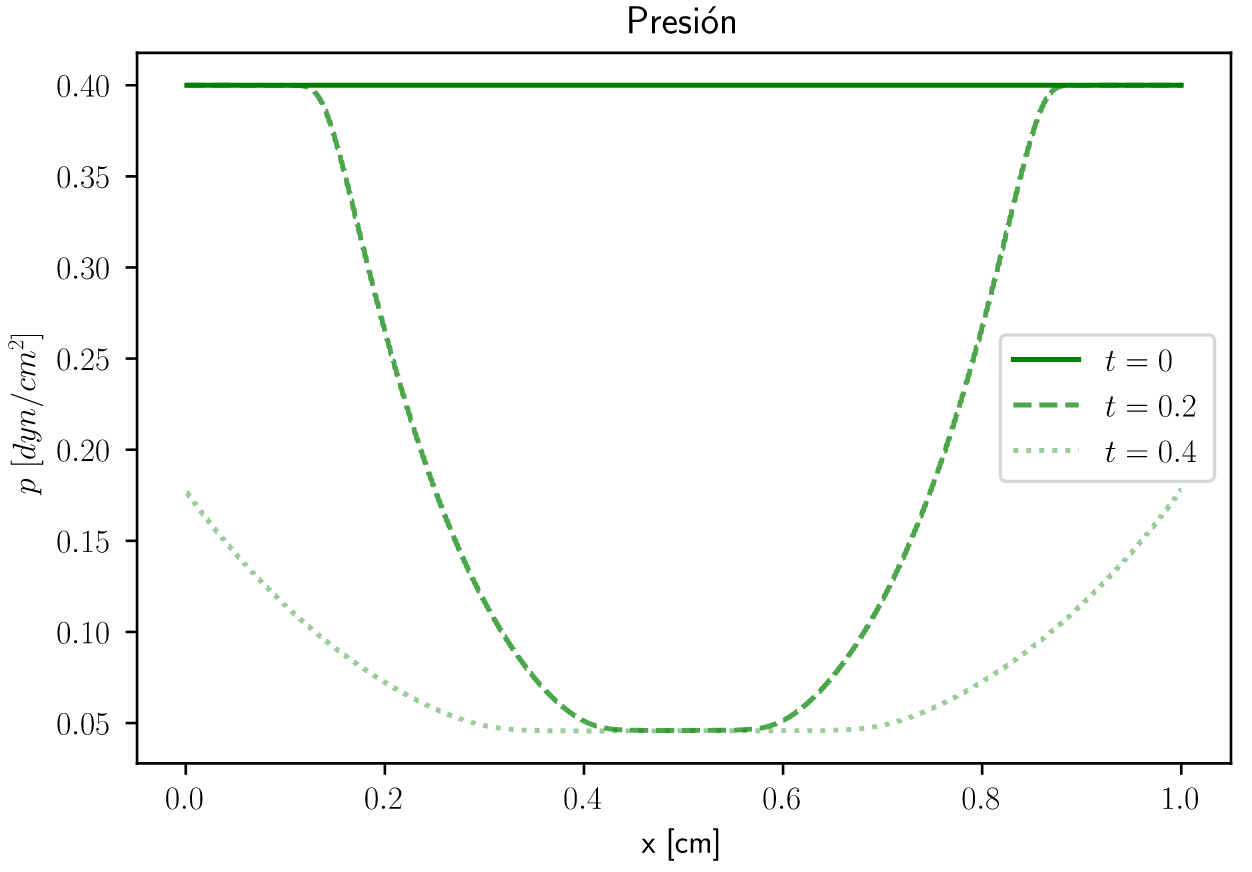
\includegraphics[scale = 0.16]{./Figuras/verificacion_del_codigo/caso_newtoniano/caso_new_rar_rar_p.png}}
    \caption{ Igual que en la Figura \ref{caso_new_rar_shock} pero para el caso 2 newtoniano. 
    El índice adiabático sigue siendo $\Gamma = 7/5$
    \label{caso_new_rar_rar}.}
\end{figure}

Para los valores $t = 0$ s, la densidad ($\rho$) y la presión ($p$) son las mismas, 
mientras que para el panel de
la velocidad  tiene una discontinuidad en $x = 0.5$ cm. 
Para el tiempo $t = 0.2$ s se puede ver una 
simetría ya que, la cabeza de la onda de rarefacción tienen lugar en los puntos $x \approx 0.16$ cm
donde la densidad $\rho = 1.0 \,  \text{g}/ \text{cm}^3$ y 
la presión $p = 0.40 \,  \text{dyn}/ \text{cm}^2 $,
decrecen hasta $\rho \approx 0.25 \,  \text{g}/ \text{cm}^3$ y $p = 0.05 \,  \text{dyn}/ \text{cm}^2 $ en forma parabólica hasta conectar con la cola de 
la onda de rarefacción, mientras que la velocidad $v = -1.0 $ cm/s decrece linealmente en magnitud 
hasta $v = 0$ cm/s. Entre los puntos $x \approx 0.4$ cm y $x \approx 0.6$ cm, que es la zona de contacto, mantienen
un valor constante para conectar con la cola de la onda de rarefacción, donde la densidad y presión 
crecen parabólicamente hasta $x \approx 0.84$ cm, mientras que la velocidad lo hace linealmente al mismo puntos.
Esa región es la cabeza de la onda y conecta con los estados iniciales del lado derecho del tubo, 
donde no ha habido perturbación, y por ende, $\rho = 1.0 \,  \text{g}/ \text{cm}^3$, 
$v = 1$ y $p = 0.4 \,  \text{dyn}/ \text{cm}^2 $.
Para el tiempo $t = 0.4$ s se aprecian las colas de las ondas de rarefacción
en los puntos $x  \approx 0.3$ y $x  \approx 0.7$, donde la densidad mantiene un valor contante 
$\rho \approx 0.25 \,  \text{g}/ \text{cm}^3$, la velocidad $v \approx 0.0$ cm/s y la presión $p = 0.05 \,  \text{dyn}/ \text{cm}^2 $.

La comparación del método de Lax y HLL se muestra en la Figura \ref{comparacion_analitico_newtoniano_caso_2}.
Como se puede ver en los paneles de densidad (arriba a la izquierda) en el punto $x \lesssim  0.05$ cm,
la densidad no está perturbada y tiene un valor $\rho = 1.0 \,  \text{g}/ \text{cm}^3$,
la velocidad (arriba a la derecha)
$v = -1.0$ cm/s y la presión (abajo a la izquierda) $p = 0.4 \,  \text{dyn}/ \text{cm}^2 $. Tanto Lax como HLL 
se ajustan casi perfectamente 
para valores constantes. Después del punto de la cabeza de la onda, los valores de la densidad y 
la presión empiezan a disminuir a $\rho \approx 0.2 \,  \text{g}/ \text{cm}^3$ y 
$p \approx 0.05 \,  \text{dyn}/ \text{cm}^2 $
en forma parabólica, mientras que la velocidad disminuye (en magnitud) linealmente hasta $v = 0$ cm/s.
Cabe señalar que los valores más bajos a los que disminuyen las magnitudes de densidad, velocidad y 
presión son en el punto $x \approx 0.33$ cm, el cual es la cola de la onda de rarefacción. Al comparar
las resoluciones, se nota que para resoluciones $\leq 1,000$ no se apega al método analítico, sobre 
todo en la cabeza de la onda.

De $x \approx 0.33$ cm, la densidad, velocidad y presión 
mantienen valores constantes de $\rho \approx 0.1 \,  \text{g}/ \text{cm}^3$, $v \approx 0$ cm/s y 
$p = 0.05 \,  \text{dyn}/ \text{cm}^2 $ 
hasta llegar al punto $x \approx 0.66$ cm donde conectan con la cola de la onda de rarefacción. En
esta región donde se enlazan las colas de la onda Lax no tiene problemas con ningún tipo de resolución.
Del punto de la cola de la onda de rarefacción de la derecha, la densidad y presión empiezan a subir 
sus valores en forma parabólica hasta a $\rho  =  1.0 \,  \text{g}/ \text{cm}^3 $ y 
a $p = 0.4 \,  \text{dyn}/ \text{cm}^2 $, 
mientras la velocidad incrementa
linealmente a $v = 1.0$ cm/s. El punto final hasta donde incrementan sus valores es la cabeza de la onda 
de rarefacción derecha, el cual es $ x \approx 0.93 $ cm.
En el panel de abajo a la derecha muestra la solución analítica, así como los resultados obtenidos 
usando Lax\footnote{
  Se usó el método de Lax porque es más rápido que HLL. 
}
con distintas resoluciones ($n_x = 10^2, \, 10^3, \,10^4$). Al igual que el caso 1 newtoniano,
conforme se incrementa la resolución, los resultados numéricos se apegan más a la solución analítica.
A partir de resoluciones mayores a 1000, los resultados se apegan mucho a la solución analítica.




\begin{figure}
  \centering
    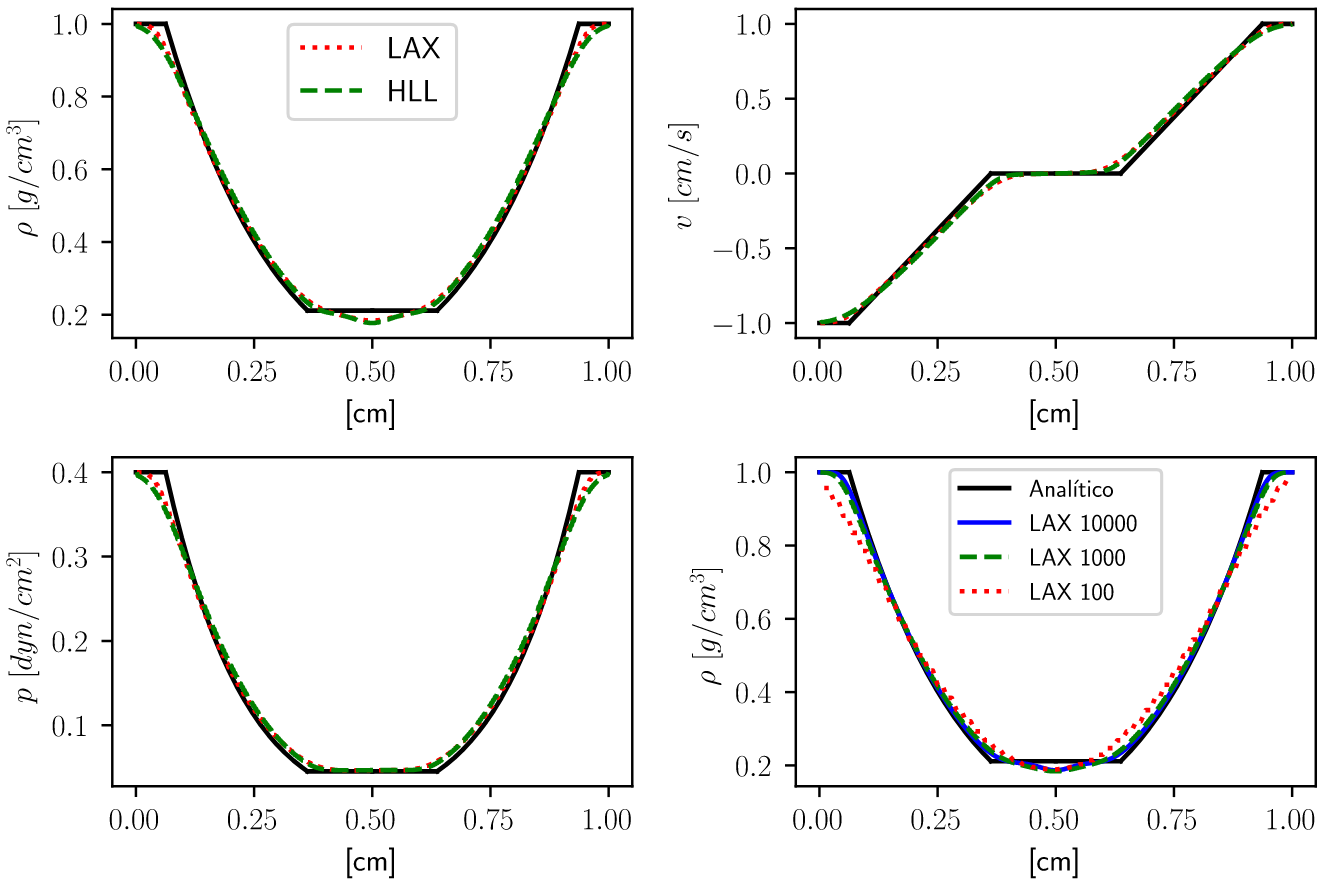
\includegraphics[width=1.0\textwidth]{./Figuras/verificacion_del_codigo/rarefaction-rarefaction.png}
  \caption{ Igual que en la Figura \ref{comparacion_analitico_newtoniano_caso_1} pero para el 
  caso 2 newtoniano a $t = 0.25$ s.
  El panel de abajo hacia la derecha muestra la comparación a distintas resoluciones para la densidad. 
  Los demás paneles muestran las diferencias de los métodos HLL y Lax con una resolución 
  de 10,000 píxeles.
  \label{comparacion_analitico_newtoniano_caso_2}} 
\end{figure}

% Para los casos newtonianos se pueden usar Lax o HLL ya que ambos se ajustan con el método analítico
% (Lora-Clavijo \emph{et. al.} 2013)
% y con una resolución $\leq 1000$ píxeles.

Podemos concluir, para el caso newtoniano, que nuestros módulos de 
Lax como HLL reproducen de forma casi perfecta la solución analítica para el problema del tubo de Sod
(Lora Clavijo \emph{et al.} 2013), ya sea en las regiones donde se muestra una discontinuidad
o donde cambia suavemente. 
Cabe destacar que el método Lax resultó ser 220 \% más rápido que HLL.
\footnote{Probado con una resolución de 10,000 píxeles con un procesador AMD Ryzen 3 3300U de
2.10 Ghz.} 

% ========================================================================================================
% ========================================================================================================


\subsection{Casos relativistas} \label{subsec:casos_relativistas_1D}

Para los casos relativistas, se tomarán valores a partir de los cuales $v \rightarrow c$,
y además se requiera usar el índice adiabático $\Gamma = 4/3$. Los valores con los que se 
toman los casos del caso relativista están en el cuadro \ref{Cuadro_parametros_sod_tube_rel} y 
cabe señalar que la velocidad de la luz está normalizada a $c = 1$  y el dominio
es $x \in [0,1]$, $x_0 = 0.5$ cm.

\begin{table}[htbp]
  \begin{center}
  \begin{tabular}{|c|c|c|c|c|c|c|}
  \hline 
  \textbf{Caso} & \textbf{$p_l$} [$\text{dyn}/\text{cm}^2$] & \textbf{$p_r$} [$\text{dyn}/\text{cm}^2$] & \textbf{$v_l$}/c & \textbf{$v_r$}/c  & \textbf{$\rho_l$} [$\text{g}/\text{cm}^3$]& \textbf{$\rho_r$} [$\text{g}/\text{cm}^3$]\\ 
  \hline 
  Caso 1 & 13.33  & 0.0  & 0.0 & 0.0 & 10  & 1 \\ 
  \hline 
  Caso 2 & 0.05  & 0.05  & -0.2 & 0.2 & 0.1  & 0.1  \\ 
  \hline 
  \end{tabular}
  \caption{\label{Cuadro_parametros_sod_tube_rel} Valores iniciales 
  de la presión ($p$), velocidad ($v$)
  y densidad ($\rho$), del lado izquierdo ($p_l, v_l, \rho_l$) y derecho ($p_r, v_r, \rho_r$)
  para los casos relativistas. Para todos los
  casos el dominio espacial será $x \in [0,1]$, la 
  posición crítica será $x_0 = 0.5$ y un índice adiabático $\Gamma = 4/3$}
  \end{center}
\end{table}

Tanto en el caso 1 relativista como el caso 2 relativista, la evolución temporal se hará usando 
el método de HLL, ya que es más preciso que el método de Lax\footnote{
  Lax falla al tratar de simular las condiciones iniciales de este problema.
}. 
Además de que necesita de altas resoluciones $\geq 10,000$ píxeles para poder funcionar.

\begin{figure}
  \centering
      \subfigure{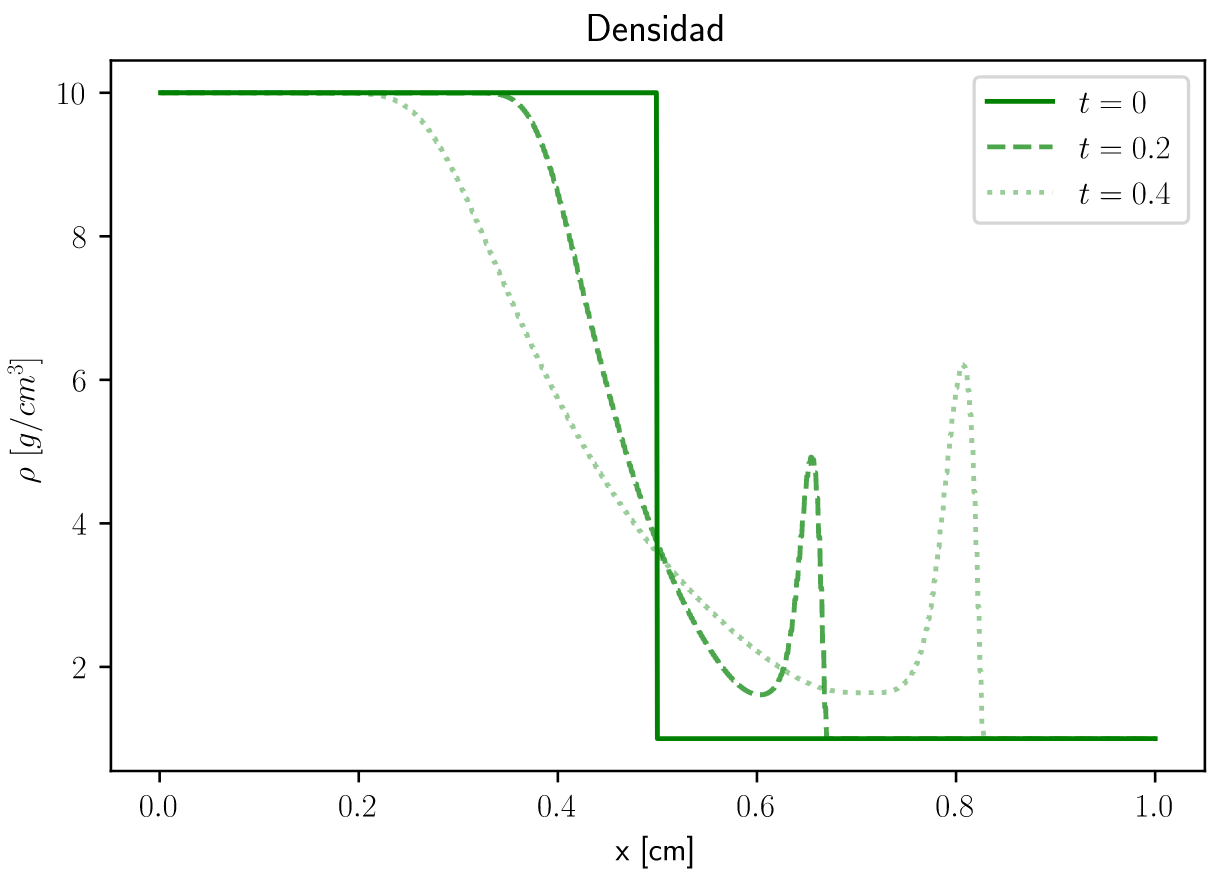
\includegraphics[scale = 0.16]{./Figuras/verificacion_del_codigo/caso_relativista/caso_rel_rar_shock_rho.png}}
      \subfigure{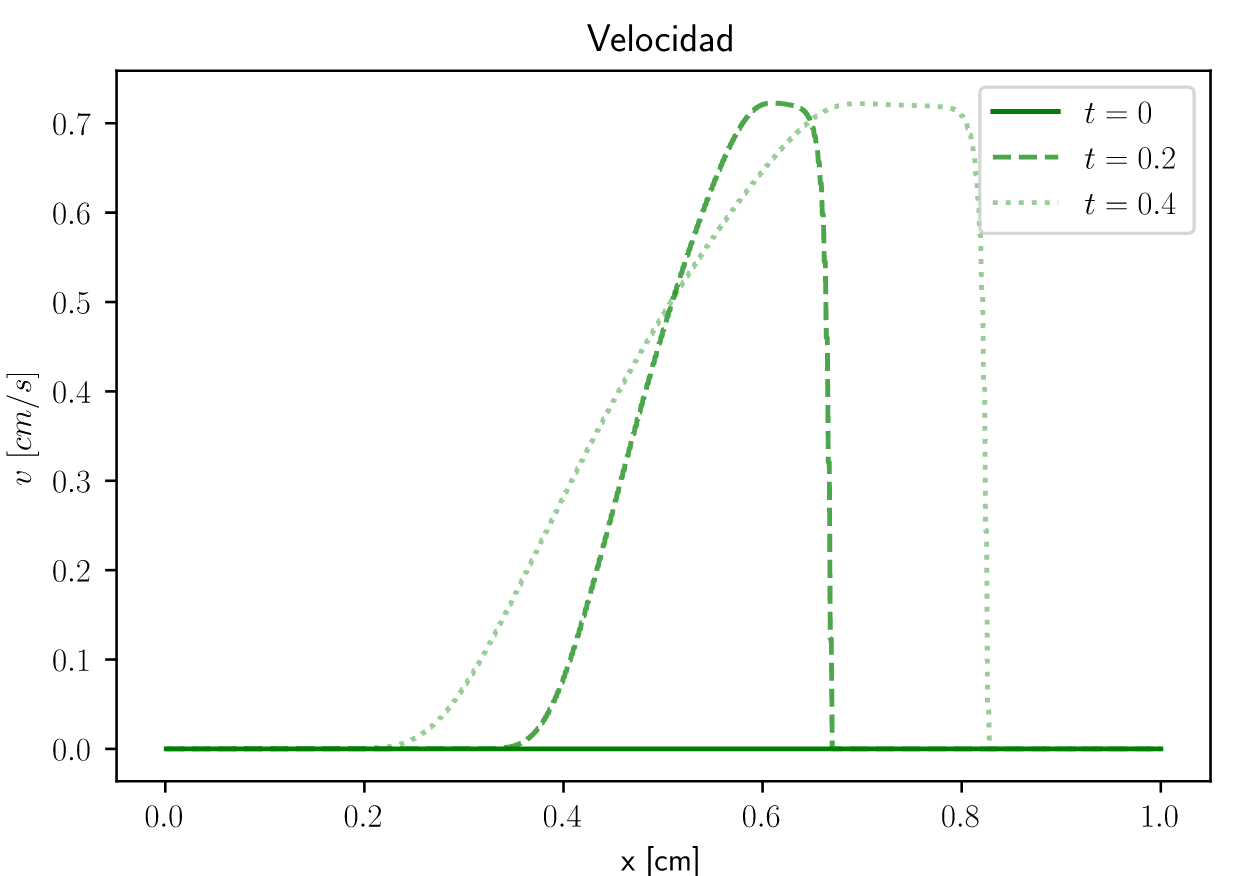
\includegraphics[scale = 0.16]{./Figuras/verificacion_del_codigo/caso_relativista/caso_rel_rar_shock_v.png}}
      \subfigure{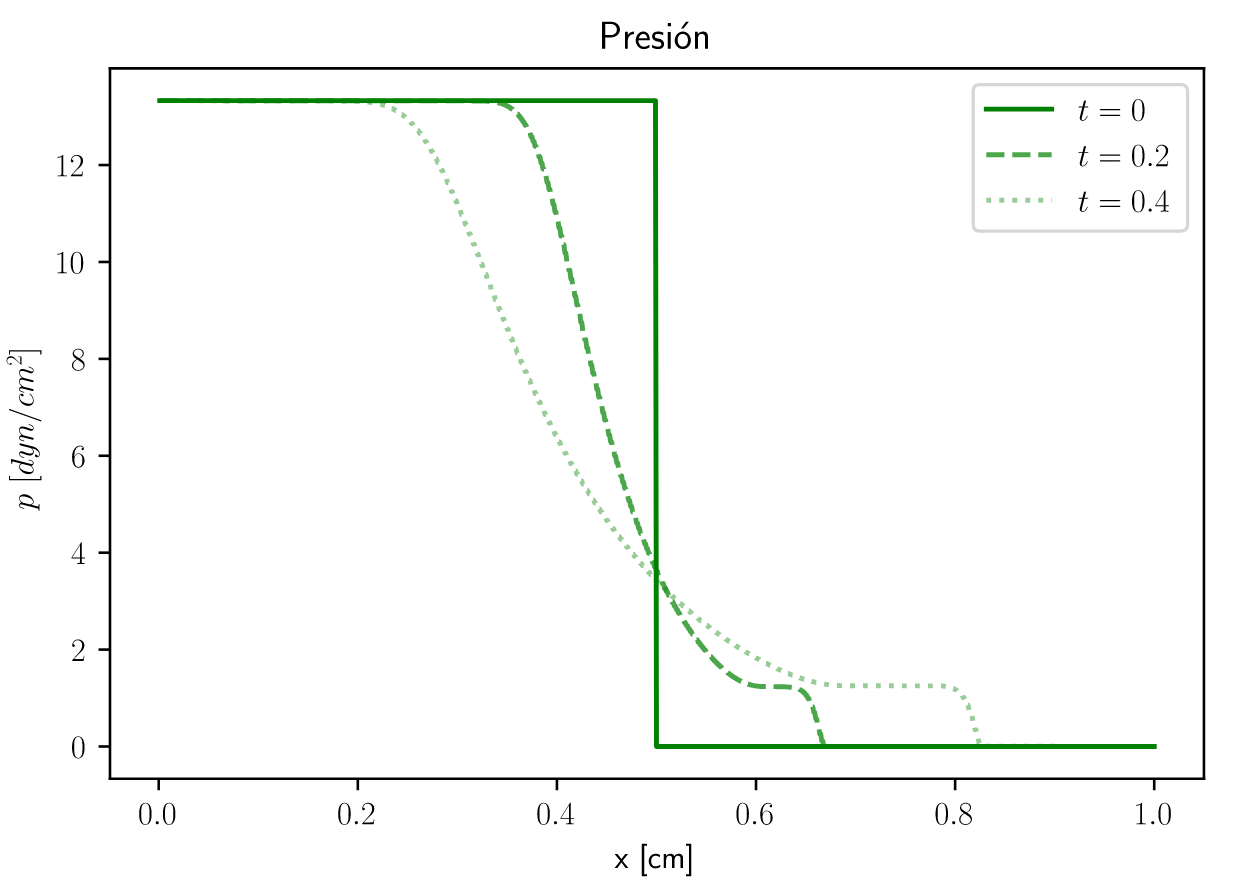
\includegraphics[scale = 0.16]{./Figuras/verificacion_del_codigo/caso_relativista/caso_rel_rar_shock_p.png}}
    \caption{Igual que en la Figura \ref{caso_new_rar_shock} pero para el caso 1 relativista. A diferencia 
    del caso newtoniano, en el relativista se usa un índice 
    adiabático $\Gamma = 4/3$. \label{caso_rel_rar_shock_1}}
\end{figure}

En la Figura \ref{caso_rel_rar_shock_1} se muestra la evolución temporal de la $\rho$, $p$ y $v$
cuando $t = 0$ s el panel de la densidad 
(arriba a la izquierda) 
y presión (abajo) presentan una discontinuidad en $x = 0.5$ cm donde $\rho = 10 \,  \text{g}/ \text{cm}^3$
y $p = 13.33 \,  \text{dyn}/ \text{cm}^2 $ del lado izquierdo, mientras que del lado derecho $\rho = 0  \,  \text{g}/ \text{cm}^3$
y $p = 0 \,  \text{dyn}/ \text{cm}^2 $. La velocidad no presenta discontinuidad y mantiene su 
velocidad nula en toda la región del tubo. 
Al tiempo $t =0.2$ s la densidad y presión 
descienden linealmente, mientras que la velocidad asciende en $x \approx 0.38$ cm
que viene siendo la cabeza de la onda de rarefacción. El punto donde alcanzan 
sus máximos y mínimos es la cola de la onda que está situada en el punto $x \approx 0.58$ cm,
la densidad y presión llegan a $\rho \approx 1.12 \,  \text{g}/ \text{cm}^3$ y 
$p \approx 1.12\,  \text{dyn}/ \text{cm}^2 $ mientras que la velocidad
va aumentando hasta llegar a $v \approx 0.75c$. La densidad vuelve a subir en el punto $x \approx 0.63$ cm
y llega a $\rho = 5.6  \,  \text{g}/ \text{cm}^3$ mientras que la velocidad y presión se mantienen iguales. Para el punto
$x \approx 0.68$ cm, la densidad, presión y velocidad bajan a valores nulos, que es la zona del tubo que
no ha sido perturbada por la onda.
Para el tiempo $t = 0.4$ s, la densidad y presión, que mantienen sus valores de 
$\rho = 10 \,  \text{g}/ \text{cm}^3$ y 
$p = 13.33 \,  \text{dyn}/ \text{cm}^2 $ bajan sus valores en $x \approx 0.25$ cm, mientras que la velocidad, la cual es nula,
asciende. En el punto $x \approx 0.68$ cm la presión alcanza $p \approx 1.12\,  \text{dyn}/ \text{cm}^2 $ y la densidad
$\rho \approx 1.12 \,  \text{g}/ \text{cm}^3$, mientras que la velocidad sube a $v \approx 0.75c$. 
La densidad vuelve a subir
en $x \approx 0.75$ cm y llega a $\rho \approx 0.65 \,  \text{g}/ \text{cm}^3$, manteniendose así hasta el punto $x \approx 0.83$ cm
donde la densidad, así como la velocidad y presión, descienden sus valores a nulos.

En la Figura \ref{caso_rel_rar_shock} se muestra la comparación entre la solución obtenida con HLL
(1000 píxeles) y la solución analítica.
El panel de arriba a la izquierda muestra la densidad, el de 
arriba a la derecha la velocidad y la presión es el de abajo a la izquierda. Cabe recalcar que  el 
tiempo mostrado es  $t = 0.35$ s.
A la región $x \lesssim 0.33$ cm, la densidad tiene un valor $\rho = 10 \,  \text{g}/ \text{cm}^3$, 
la presión $p = 13.33 \,  \text{dyn}/ \text{cm}^2 $
y la velocidad es nula. Se puede ver que HLL se ajusta casi perfectamente para los valores constantes
sin importar la resolución. 
En el punto $x \approx 0.33$ cm se localiza la cabeza de la onda, donde la presión y la densidad 
empiezan a decaer en forma parabólica, mientras que la velocidad comienza subir en forma linealmente.
El punto donde la densidad y presión alcanzan su mínimo, mientras que la velocidad, su máximo,
se localiza en $x \approx 0.62$ cm. La resolución para esta región es $\geq 500$ 
píxeles. En el punto $x \approx 0.75$ cm, 
la densidad tiene una discontinuidad, al cual se le conoce como discontinuidad de la onda de contacto.
Debido a esta región la resolución a tomar en cuenta debe ser $\geq 1,000$ o incluso $\geq 10,000$.
En esta discontinuidad la densidad pasa de $ \rho \approx 3 \,  \text{g}/ \text{cm}^3$ a
$ \rho \approx 9 \,  \text{g}/ \text{cm}^3$ mientras que la presión 
y velocidad se mantienen en $p \approx 2\,  \text{dyn}/ \text{cm}^2 $ 
y $v = 0.75$ c. La última discontinuidad que es la de choque,
todas las magnitudes ($\rho$, $v$ y $p$) disminuyen a su valor nulo y la resolución a tomar en cuenta
puede ser $\geq 1,000$ píxeles dado que HLL no presenta dificultades con esta discontinuidad.

En el panel de abajo a la derecha muestra la solución analítica, así como los resultados obtenidos 
usando HLL con distintas resoluciones ($n_x = 10^2, \, 10^3, \,10^4$).
Se puede observar, que aunque apenas es visible en 1D, el método de HLL es un poco más aproximado a la solución analítica.  
En específico, para el problema 1 relativista, a partir de resoluciones mayores a 1000, los
resultados se apegan mucho a la solución analítica.


\begin{figure}
  \centering
    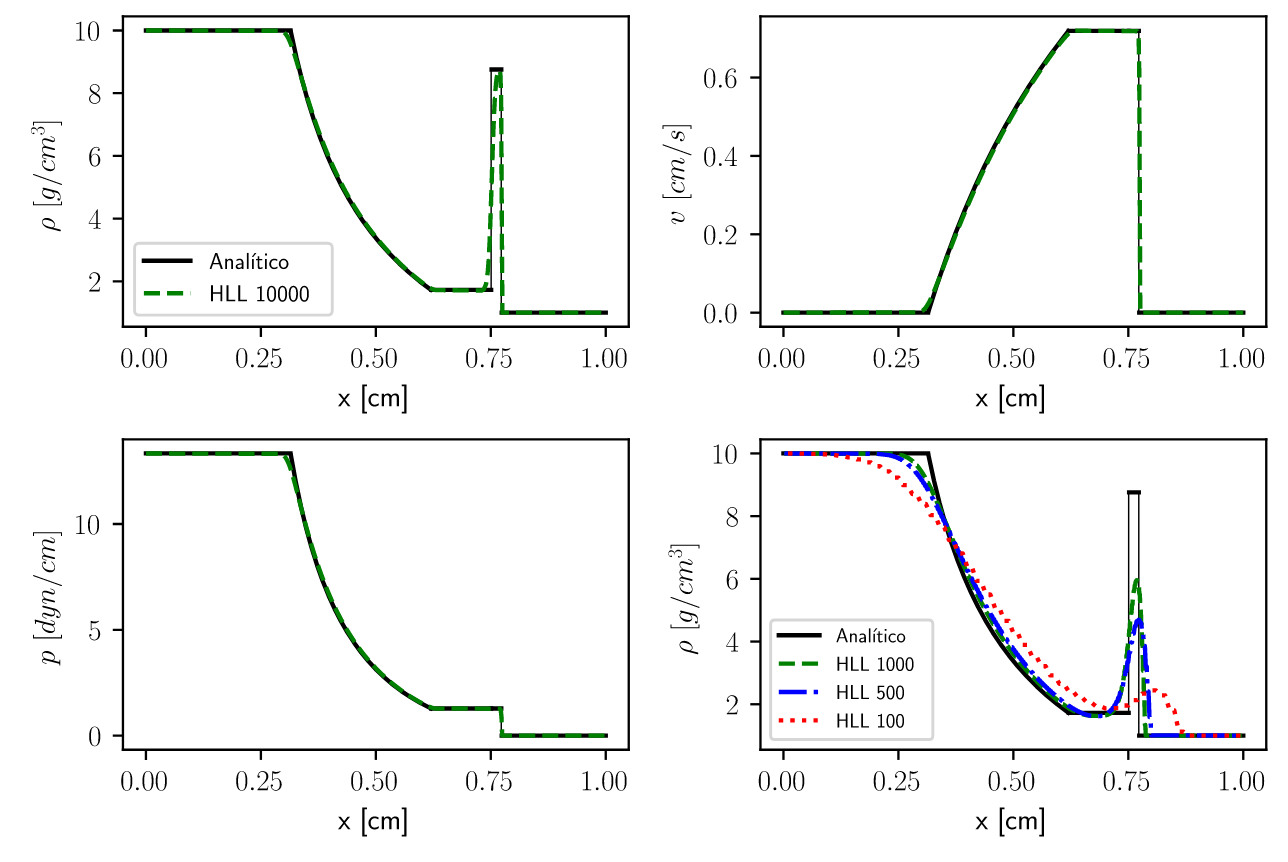
\includegraphics[width=1.0\textwidth]{./Figuras/verificacion_del_codigo/caso_relativista/caso_rel_rar_shock.png}
  \caption{Igual que en la Figura \ref{comparacion_analitico_newtoniano_caso_1} pero para el caso 1 
  relativista 
  a $t = 0.35$ s. El panel de abajo 
  hacia la
  derecha muestra la comparación a distintas resoluciones para la densidad. Los demás paneles muestran
  las diferencias de los métodos HLL y Lax con una resolución de 10,000.}\label{caso_rel_rar_shock}
\end{figure}

%=========================================================================================================

El caso 2 relativista representa 2 ondas de rarefacción, a diferencia del caso 1 las velocidades que 
alcanzan las 
ondas no son velocidades relativistas.
\begin{figure}
  \centering
      \subfigure{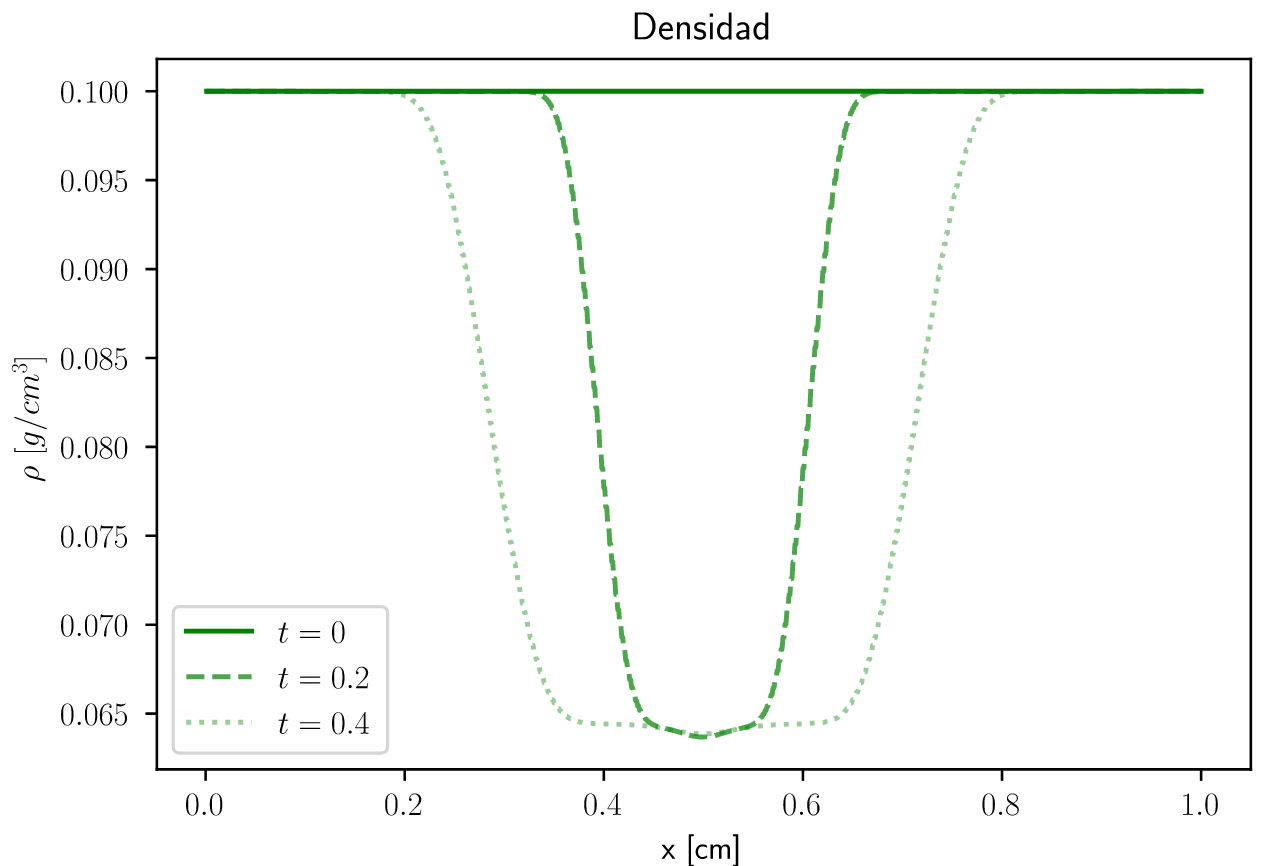
\includegraphics[scale = 0.16]{./Figuras/verificacion_del_codigo/caso_relativista/caso_rel_rar_rar_rho.png}}
      \subfigure{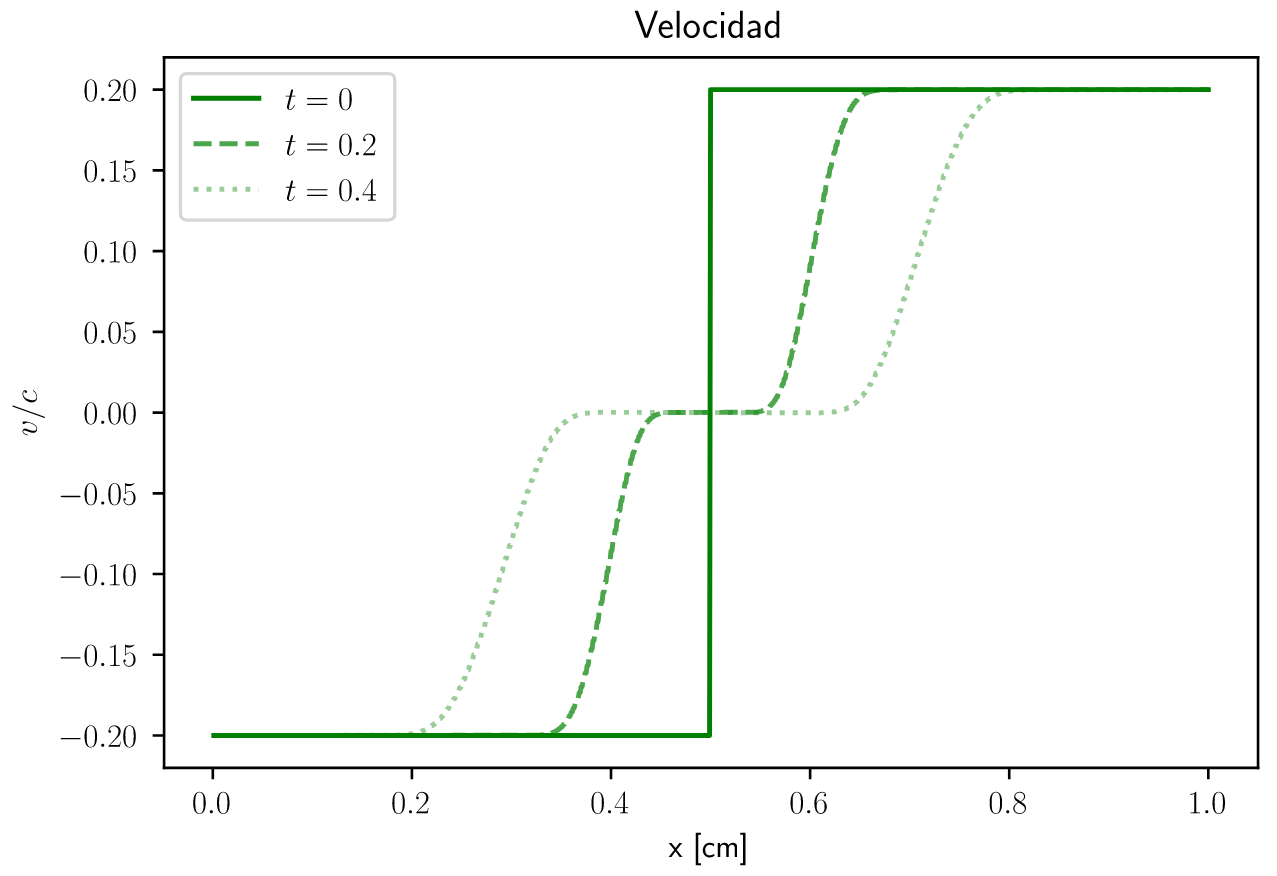
\includegraphics[scale = 0.16]{./Figuras/verificacion_del_codigo/caso_relativista/caso_rel_rar_rar_v.png}}
      \subfigure{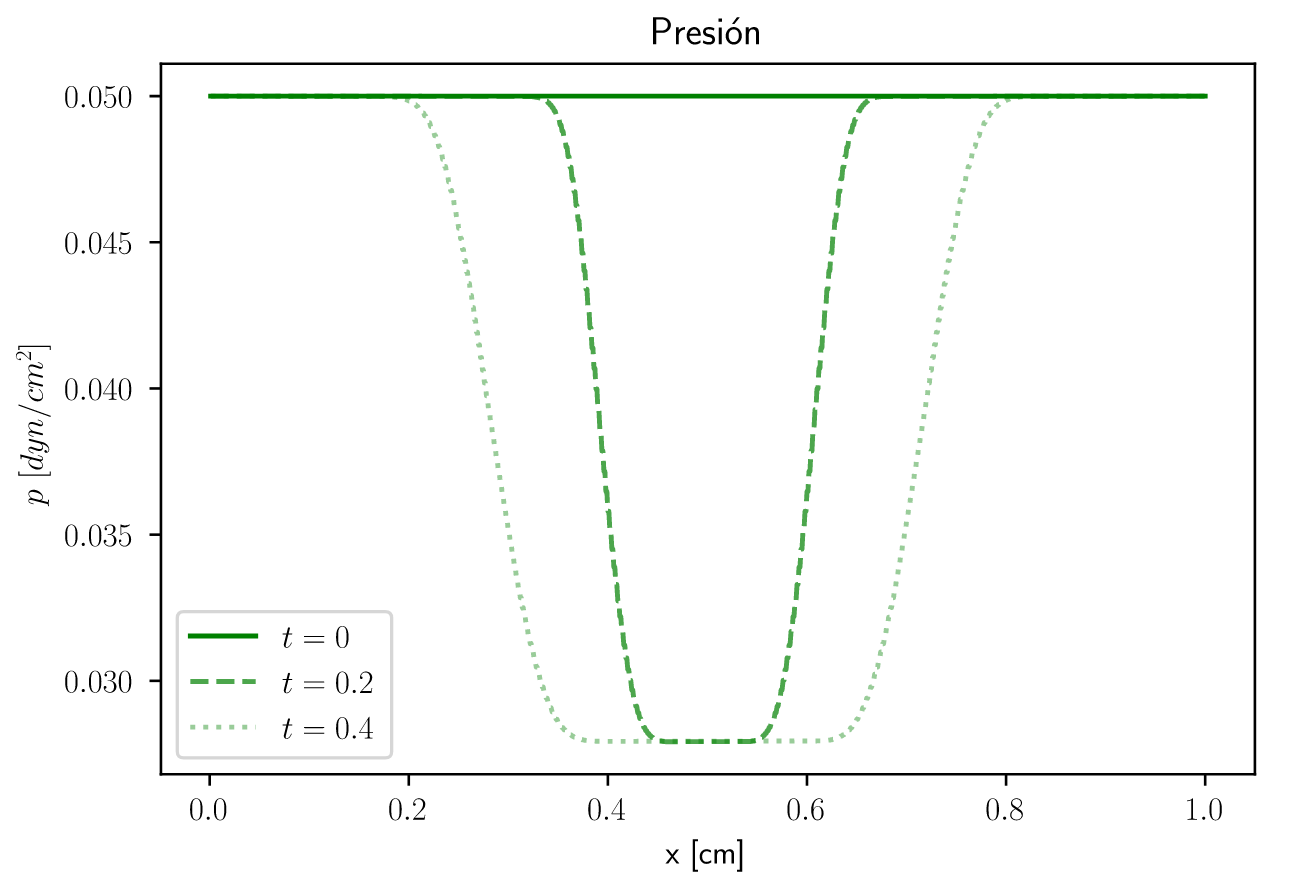
\includegraphics[scale = 0.16]{./Figuras/verificacion_del_codigo/caso_relativista/caso_rel_rar_rar_p.png}}
    \caption{Igual que en la Figura \ref{caso_new_rar_shock} pero para el caso 2 relativista. 
    El panel de arriba a la izquierda muestra la densidad.
    El de arriba a la derecha la velocidad y el de abajo la presión}\label{caso_rel_shock_shock}
\end{figure}
A diferencia del caso 1 relativista, el caso 2 relativista no presenta discontinuidades,
por lo que se pueden usar resoluciones $\leq 100$ píxeles. En la Figura 
\ref{caso_rel_shock_shock},  
el panel de arriba a la izquierda muestra la densidad, el de arriba a la derecha la velocidad
y el de abajo la presión.
Al igual que el caso newtoniano, al simular las 2 ondas presenta una simetría con respecto a la 
discontinuidad.
En el tiempo $t = 0$ s, tanto la densidad como la presión mantienen los mismos valores 
$\rho =0.1 \,  \text{g}/ \text{cm}^3$
y $p = 0.05$, mientras que la velocidad tiene una discontinuidad en $x = 0.5$ cm, donde la parte del lado
izquierdo de la discontinuidad es $v = -0.2$ c,  (el signo negativo solo muestra que las ondas de choque
tienen una dirección opuesta entre sí). 
Mientras que del lado derecho es $v = 0.2$ c.
Al tiempo $t = 0.2$ s, la cabeza de la onda de rarefacción se presenta en los puntos 
$x \approx 0.35$ cm, donde los valores de la presión $p = 0.05$ y densidad 
$\rho =0.1 \,  \text{g}/ \text{cm}^3$ comienzan a descender linealmente,
mientras que la velocidad $v = 0.2$ c desciende hasta el punto $x \approx 0.45$ cm. En este punto los valores de la densidad, presión y velocidad
son $\rho \approx 0.065 \,  \text{g}/ \text{cm}^3$, $p \approx 0.028\,  \text{dyn}/ \text{cm}^2 $ 
y $v \approx 0$ c. Los valores cambian en 
$ x \approx 0.55$ cm
que es la cola de la onda de rarefacción derecha, y comienzan a subir
hasta $x \approx 0.65$ cm donde ahora la densidad es 
$\rho = 0.1 \,  \text{g}/ \text{cm}^3$, la presión $p = 0.05 \,  \text{dyn}/ \text{cm}^2 $ y 
la velocidad $v = 0.2$ c.
Para el tiempo $t = 0.4$ s se sigue manteniendo el mismo sistema que al tiempo $t =0.2$ s, ya que en
$x \approx 0.25$ cm los valores de la densidad $\rho = 0.1 \,  \text{g}/ \text{cm}^3$, 
presión $p = 0.05 \,  \text{dyn}/ \text{cm}^2 $ 
y velocidad $v = -0.2$ c descienden en forma lineal hasta el punto $x \approx 0.35$ cm, donde 
se mantienen constantes los valores $\rho \approx 0.065  \,  \text{g}/ \text{cm}^3$, 
$p \approx 0.028\,  \text{dyn}/ \text{cm}^2 $ y $v \approx 0$ c 
hasta el punto $x \approx 0.65$ cm donde vuelven a ascender linealmente
hasta el punto $x = 0.75$ cm donde los valores regresan a $\rho = 0.1 \,  \text{g}/ \text{cm}^3$, 
$p = 0.05 \,  \text{dyn}/ \text{cm}^2 $ y la velocidad 
cambia de sentido $v = 0.2$ c.


\begin{figure}
  \centering
    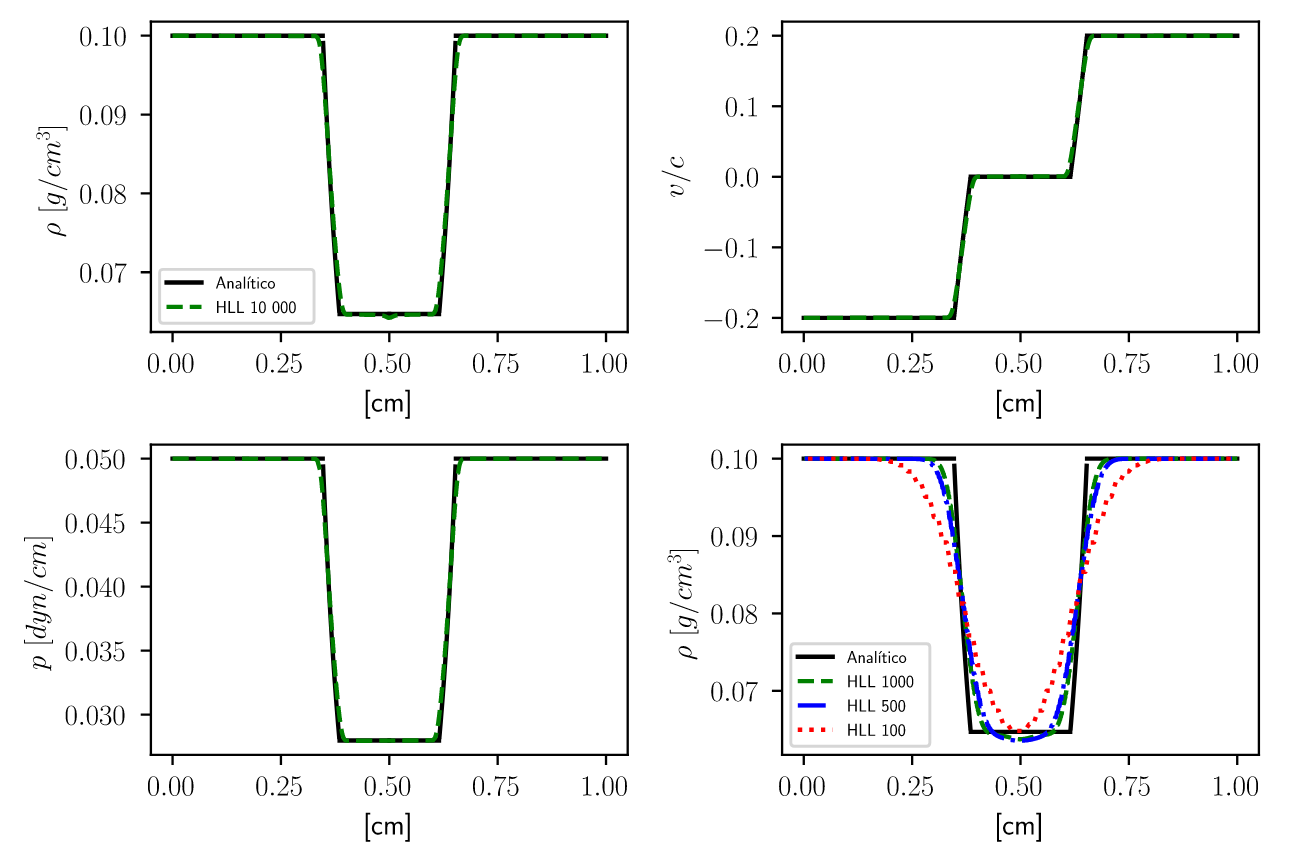
\includegraphics[width=1.0\textwidth]{./Figuras/verificacion_del_codigo/caso_relativista/caso_rel_rar_rar.png}
  \caption{Igual que en la Figura \ref{comparacion_analitico_newtoniano_caso_1} pero para el caso 2 
  relativista. Se usó un índice adiabático $\Gamma = 4/3$ y $t = 0.25$ s.
  } \label{caso_rel_shock_shock_2}
\end{figure}

En la Figura \ref{caso_rel_shock_shock_2}, el panel de arriba a la izquierda muestra el perfil de la 
densidad, el de arriba a la derecha la velocidad, el de abajo a la izquierda la presión. Esos 3 muestran
una comparación entre el método analítico y el método numérico (HLL) usando una resolución de 
10,000 píxeles. 
En $x \lesssim 0.33$ cm los valores de la densidad, presión y velocidad son 
$\rho = 0.1 \,  \text{g}/ \text{cm}^3$, $p = 0.05 \,  \text{dyn}/ \text{cm}^2 $
y $v = -0.2$ c. HLL para resoluciones $\geq 500$ se ajusta perfectamente al analítico. Cuando los 
valores descienden en $x \approx 0.37$ cm a $\rho \approx 0.065 \,  \text{g}/ \text{cm}^3$, 
$v \approx 0$ c y $p \approx 0.025\,  \text{dyn}/ \text{cm}^2 $. En
esta región podemos ver que para resoluciones $\leq 100$ píxeles se tiene dificultades para apegarse al
método analítico, sobre todo en las regiones de la cabeza y cola de la onda de rarefacción. En el punto $x \approx 0.63$  cm tanto la presión como la densidad y la velocidad vuelven a subir
sus valores hasta el punto $x \approx 0.65$ cm donde alcanzan los valores que tenía del lado izquierdo
donde la densidad ahora es $\rho = 0.1 \,  \text{g}/ \text{cm}^3$, la presión $p = 0.05 \,  \text{dyn}/ \text{cm}^2 $ 
y la velocidad $v = 0.2$ c.
En el panel de abajo a la derecha se muestra la solución analítica, así como los resultados obtenidos 
usando HLL con distintas resoluciones ($n_x = 10^2, \, 10^3, \,10^4$). 
Al igual que el caso 1 relativista,
conforme se incrementa la resolución, los resultados numéricos se apegan más a la solución analítica.
A partir de resoluciones mayores a 1000, los resultados se apegan mucho a la solución analítica.
Por lo tanto, podemos concluir que nuestro módulo HLL se ajusta perfectamente para el problema de 
Riemann relativista con resoluciones $\geq 500$ píxeles.

% ===============================================================================================
% ===============================================================================================


\section{Pruebas bidimensionales}

\subsection{Caso Newtoniano (Sedov-Taylor)}\label{subsec:caso_newtoniano_2d}

En esta sección se verifica que el código newtoniano reproduja correctamente la expansión de la onda bidimensional de Sedov-Taylor (en la que se libera una gran cantidad de energía en un volumen muy pequeño, 
y la cual es discutida a fondo en la Sección 2.5). Para lo anterior, se inyecta instantáneamente una gran cantidad de energía \emph{E} dentro de un radio R inmerso en un medio ambiente de densidad uniforme $\rho_m$. 
Posteriormente, un frente de choque bidimensional se expande a través del medio ambiente. El radio inicial de la onda es $r = 2$ pc, y el dominio computacional fue de 
$x, y \in [0,4 \times 10^{20}]\times[0,4 \times 10^{20}] \, \text{cm}$. La resolución fue de 1000x1000 píxeles, se tomó un índice adiabático $\Gamma = 5/3$, y el tiempo de integración 
fue $t = 8.1 \times 10^{10}$ s. Dentro del radio inicial la densidad, presión, y velocidades fueron: $\rho_s, p_s, v_{xs}, v_{ys}$, para el medio ambiente la densidad, presión, y velocidades fueron: 
$\rho_m, p_m, v_{xm}, v_{ym}$. Los valores típicos de una supernova con energía $E_{s}  \approx 10^{52}$ ergs están mencionados en el Cuadro \ref{Cuadro_parametros_choque_2D_newtoniano}:

\begin{table}[htbp]
  \begin{center}
  \begin{tabular}{|c|c|c|c|c|c|c|c|c|}
  \hline 
  \textbf{Unidades} & \textbf{$p_s$} [$\text{dyn}/\text{cm}^2$] & 
  \textbf{$p_m$} [$\text{dyn}/\text{cm}^2$] & 
  $\frac{v_{xs}}{c}$ & $\frac{v_{xm}}{c}$  & $\frac{v_{ys}}{c}$ & $\frac{v_{ym}}{c}$  & 
  \textbf{$\rho_s$} [$\text{g}/\text{cm}^3$]& 
  \textbf{$\rho_m$} [$\text{g}/\text{cm}^3$]\\ 
  \hline 
  valores & $2.01 \times 10^{-6}$ & $8.97 \times 10^{-10}$  & 0 & 0 & 0 & 0 &  $3.48 \times 10^{-24}$  & $1.67 \times 10^{-24}$ \\ 
  \hline 
  \end{tabular}
  \caption{\label{Cuadro_parametros_choque_2D_newtoniano} Valores iniciales 
  de la presión, velocidad, y densidad ($\rho$), dentro de R ($p_s, v_{xs}, v_{ys}, \rho_s$) y del medio ambiente ($p_m, v_{xm}, v_{ym}, \rho_m$) para el problema de Sedov-Taylor.}
  \end{center}
\end{table}

La Figura \ref{fig:prueba_2d_newtoniana} muestra la evolución de la onda. El panel de arriba a la izquierda muestra la onda de choque al tiempo $t = 0$, el panel de arriba a la derecha muestra 
la evolución al tiempo $t = 10^{10}$ s, y la de abajo al tiempo $t =8.1 \times 10^{10}$ s. En estos se observa como a $10^{10}$ s y a $8.1 \times 10^{10}$ s la onda tiene un radio de $\sim 1.6$ pc y $\sim 4.5$ pc, 
respectivamente. En ambos tiempos la explosión es esférica y se tiene una sobredensidad de $\rho \approx 3.5 \times 10^{-24} \text{g} \, \text{cm}^{-3}$ en el perímetro de la onda, mientras que dentro de la onda 
la densidad decae a $\rho \approx 10^{-24} \text{g} \, \text{cm}^{-3}$.

\begin{figure}
  \centering
      \subfigure{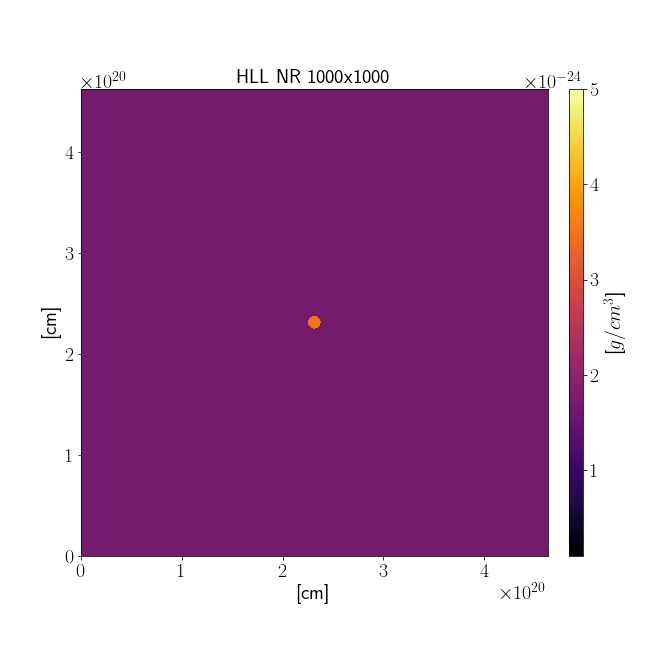
\includegraphics[scale = 0.3]{./Figuras/verificacion_del_codigo/prueba_2d_newtoniana/0_NR.png}}
      \subfigure{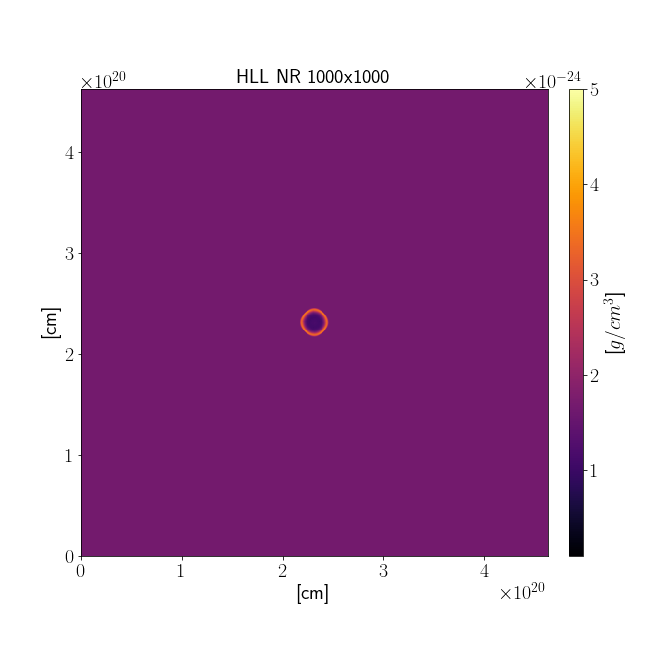
\includegraphics[scale = 0.3]{./Figuras/verificacion_del_codigo/prueba_2d_newtoniana/11_NR.png}}
      \subfigure{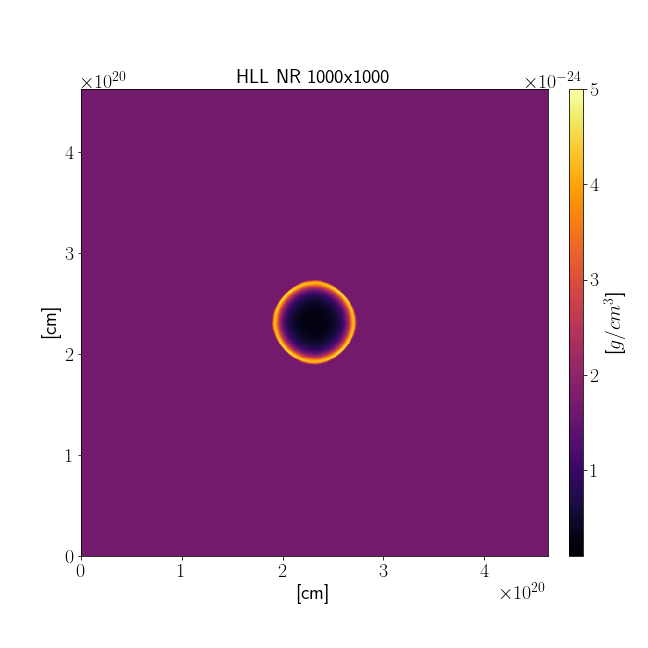
\includegraphics[scale = 0.3]{./Figuras/verificacion_del_codigo/prueba_2d_newtoniana/99_NR.png}}
    \caption{Mapas de densidad mostrando la evolución de la onda de choque de Sedov-Taylor en 2 dimensiones. El panel de arriba a la izquierda muestra el tiempo inicial $t=0$ s, el de arriba a la derecha al 
    $t \approx 10^{10}$ s, y el panel de abajo muestra el tiempo $t = 8.1 \times 10^{10}$ s.
    \label{fig:prueba_2d_newtoniana}}
\end{figure}

Para verificar que el código HD estaba reproduciendo correctamente la solución analítica de Sedov-Taylor se comprobó que el radio de la onda de expansión de la simulación siguiese la solución analítica 
dada en la ecuación \ref{eq_Radio_proporcional}, esto es, que el radio de la onda creciera como $r\propto t^{2/5}$. La Figura \ref{fig:Expansion_HLL_NR} muestra la evolución del radio de la onda en función del tiempo (verde) así como 
la curva que mejor se le ajusta (rojo). La curva que mejor se ajusta a los datos resultó ser $r(t) = t^{0.413}$. El coeficiente de determinación fue $R^2= 0.985$ lo cual nos indica que el modelo se ajusta muy bien a 
los datos de la simulación. Al comparar nuestro modelo con la teoría podemos notar una discrepancia del 5 \%, y por ende podemos concluir que el problema de Sedov-Taylor fue resuelto correctamente por el código HD.

\begin{figure}
  \centering
  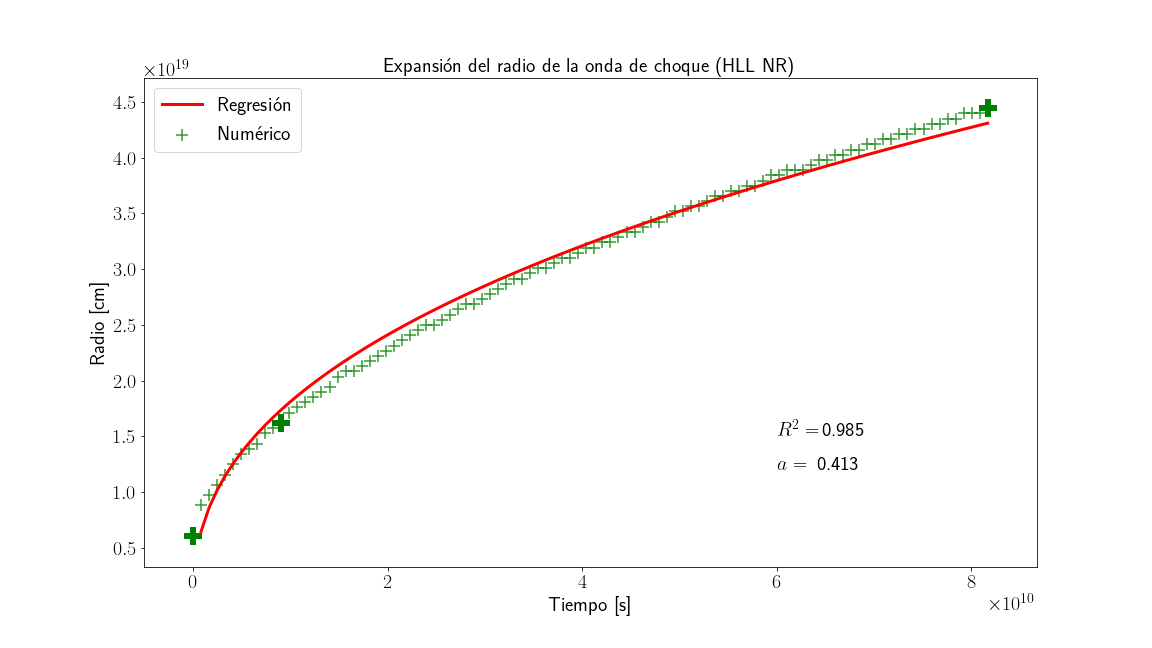
\includegraphics[width=1\textwidth]{./Figuras/verificacion_del_codigo/prueba_2d_newtoniana/Expansion_HLL_NR_res_1000.png}
    \caption{Crecimiento del radio de la onda de choque en función del tiempo. Las cruces verdes muestran la evolución del radio de la onda de choque en la simulación. La línea sólida roja muestra la curva que mejor 
    se ajusta a los datos: $r(t) = t^{0.413}$ (con un coeficiente de determinación $R^2= 0.985$). Las cruces más remarcadas corresponden a los radios que se muestran en la Figura \ref{fig:prueba_2d_newtoniana}.}
    \label{fig:Expansion_HLL_NR}
\end{figure}

\subsection{Caso relativista} \label{subsec:caso_relativista_2d}
Para verificar que el código RHD funciona correctamente en 2D se hizo una prueba de una onda de choque relativista en 2 dimensiones y se verificó que se comporta como la solución analítica auto-similar de 
una prueba de un tubo de choque bidimensional. El dominio espacial fue $x, y \in [0,1]\times[0,1] \, \text{cm}$, el radio de la 
onda $r = 0.5 \, \text{cm}$. Se consideró un índice adiabático $\Gamma = 4/3$, y una resolución de 1000x1000 píxeles. Los valores que hay dentro de la onda bidimensional, así como 
los que el medio ambiente, se muestran en el cuadro \ref{Cuadro_parametros_choque_2D}. 
\begin{table}[htbp]
  \begin{center}
  \begin{tabular}{|c|c|c|c|c|c|c|c|c|}
  \hline 
  \textbf{Unidades} & \textbf{$p_i$} [$\text{dyn}/\text{cm}^2$] & 
  \textbf{$p_o$} [$\text{dyn}/\text{cm}^2$] & 
  $\frac{v_{xi}}{c}$ & $\frac{v_{xo}}{c}$  & $\frac{v_{yi}}{c}$ & $\frac{v_{yo}}{c}$   & 
  \textbf{$\rho_i$} [$\text{g}/\text{cm}^3$]& 
  \textbf{$\rho_o$} [$\text{g}/\text{cm}^3$]\\ 
  \hline 
  Valores & 13.33  & 0.0  & 0.0 & 0.0 & 0.0 & 0.0 & 10.0  & 1.0 \\ 
  \hline 
  \end{tabular}
  \caption{\label{Cuadro_parametros_choque_2D} Valores iniciales 
  de la presión, velocidad, y densidad ($\rho$) dentro de la onda relativista ($p_i, v_{xi}, v_{yi}, \rho_i$) y del medio ambiente ($p_o, v_{xo}, v_{yo}, \rho_o$).}
  \end{center}
\end{table}

Al tiempo $t = 0$, el dominio estará dividido en 2 conjuntos, a los valores ($\rho$, $v_x$, $v_y$ y $p$) que estén en la región menor al radio serán los valores internos ($\rho_i$, $v_{x_{i}}$, $v_{x_{i}}$ y $p_i$) mientras 
que los valores que no estén delimitados por el radio serán los valores externos ($\rho_o$, $v_{x_{o}}$, $v_{x_{o}}$ y $p_o$). Al ser $p_i > p_o$ y $\rho_i > \rho_o$, la onda se  expandirá incrementando el radio, por 
lo que la región de adentro se vuelve más grande.

La Figura \ref{Example_blast_wave} muestra los perfiles de densidad (líneas negras punteadas), que se tomarán de la onda de choque en 2D, para poder comparar con los resultados de las pruebas unidimensionales, 
así como la analítica. En la Figura \ref{fig:head_map} muestra un mapa de densidades en el cual se ve la evolución de la onda. En el panel de arriba a la izquierda muestra el estado inicial al tiempo $t = 0$ s, el panel 
de arriba a la derecha muestra su estado al tiempo $t = 0.2$ s y el panel de abajo muestra su estado para $t = 0.4$ s. 

\begin{figure}
  \centering
    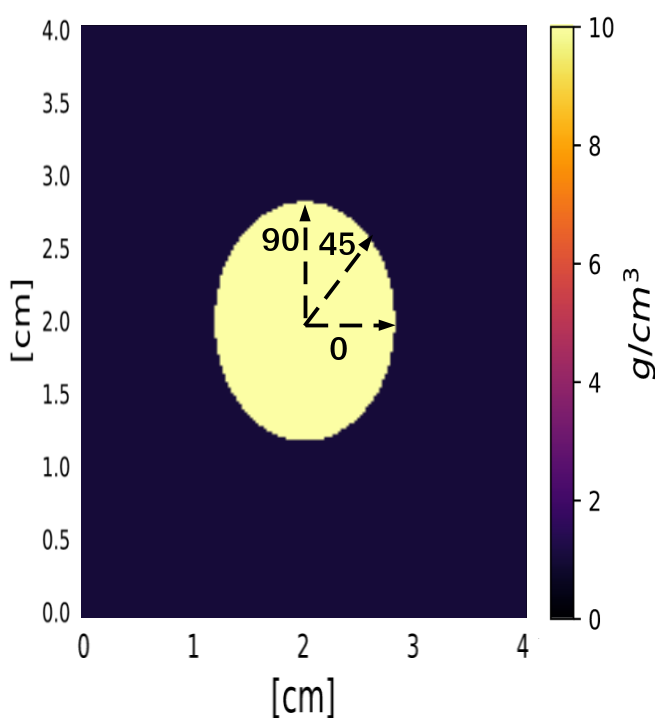
\includegraphics[width=0.4\textwidth]{./Figuras/verificacion_del_codigo/pruebas_2D/Example.png}
  \caption{Las líneas punteadas indican los perfiles de densidad, velocidad y presión que se 
  tomaran de los radios que son 
  paralelos al eje x,  perpendiculares (0°, 45°,90°) y se compararán con las pruebas en 
  1 dimensión.}\label{Example_blast_wave}
\end{figure}

\begin{figure}
  \centering
      \subfigure{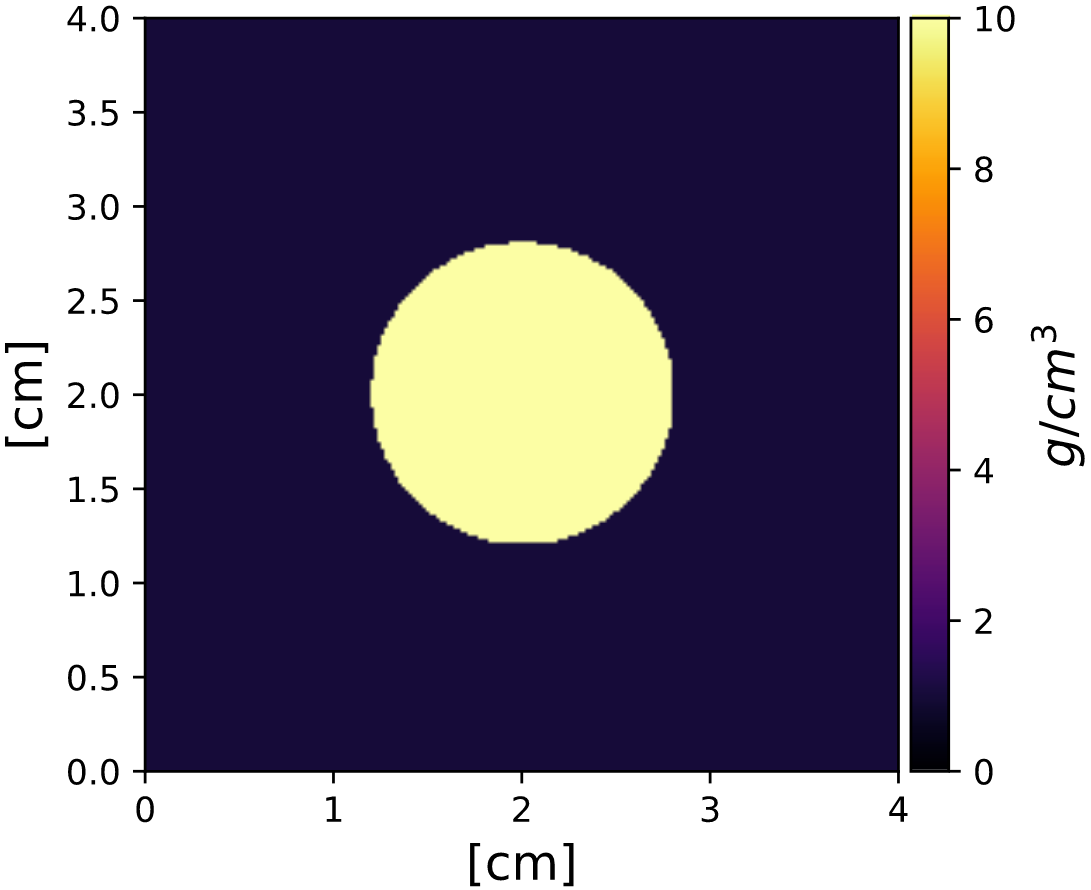
\includegraphics[scale = 0.3]{./Figuras/verificacion_del_codigo/pruebas_2D/head_map/00.png}}
      \subfigure{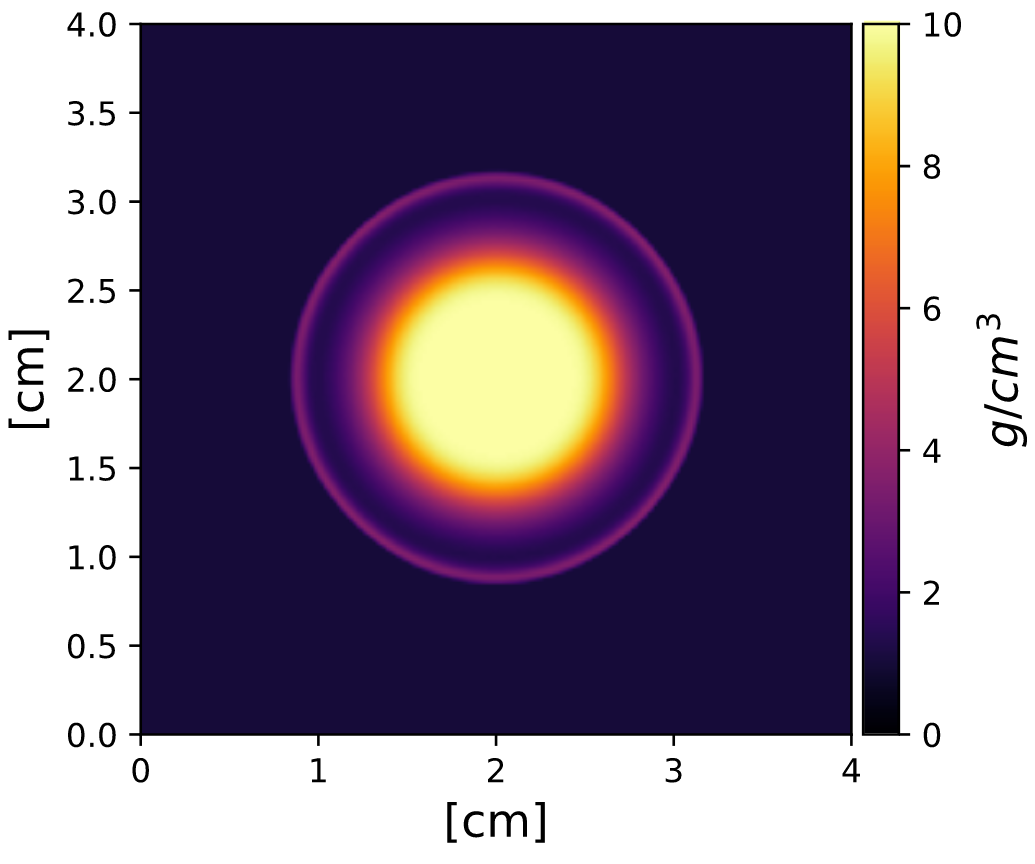
\includegraphics[scale = 0.3]{./Figuras/verificacion_del_codigo/pruebas_2D/head_map/20.png}}
      \subfigure{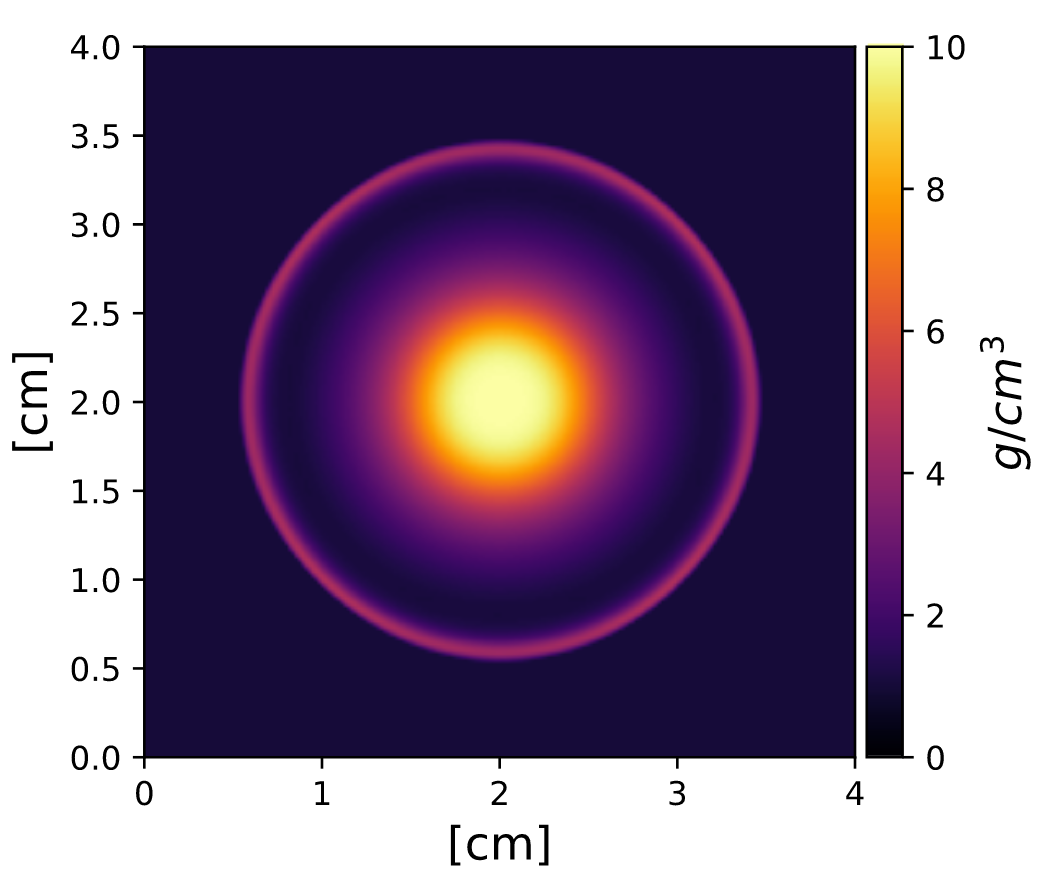
\includegraphics[scale = 0.3]{./Figuras/verificacion_del_codigo/pruebas_2D/head_map/40.png}}
    \caption{Explosión de la onda de choque en 2 dimensiones usando un mapa de calor donde muestra
    la evolución de la densidad. El panel de arriba a la izquierda muestra el tiempo inicial $t=0$ s,
    el de arriba a la derecha  al $t = 0.2$ s y el de abajo al tiempo $t = 0.4$ s. 
    \label{fig:head_map}}
\end{figure}

En la gráfica \ref{fig:Expansion_radio_vs_tiempo} se muestra la expansión del radio de la explosión de la onda de choque en función del tiempo, y se ajustó una regresión para 
poder calcular el exponente con el que crece el radio, donde se muestra que crece como $R(t) \propto t^{0.426}$ y que tiene un $R^2 = 0.946$, lo cual coincide aproximadamente con la solución newtoniana de Sedov-Taylor 
(véase la Sección \ref{subsec:caso_newtoniano_2d}).

\begin{figure}
    \begin{center}
      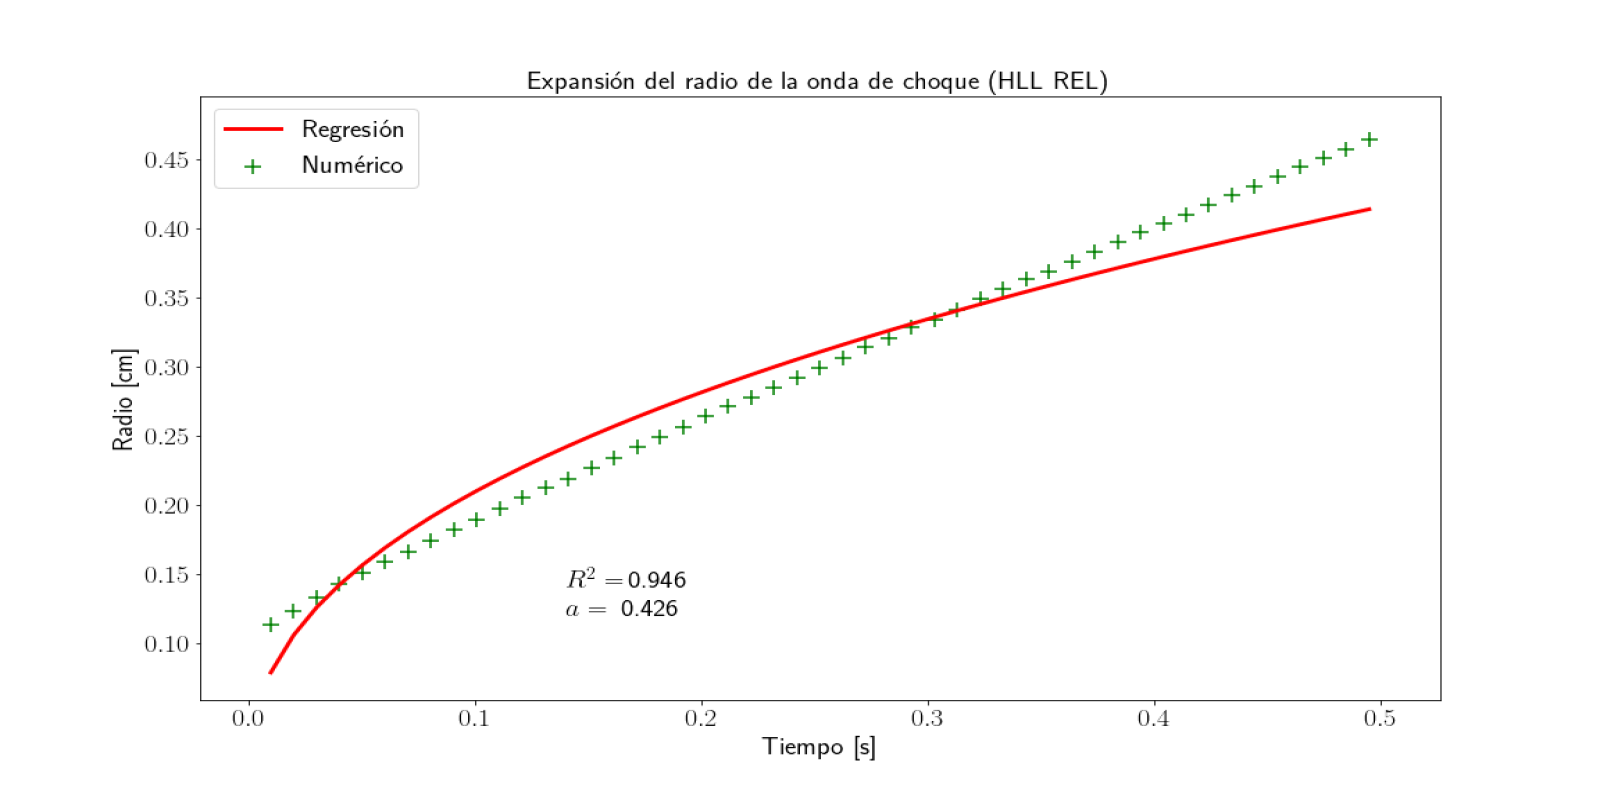
\includegraphics[width=0.95\textwidth]{./Figuras/verificacion_del_codigo/pruebas_2D/expansion_radio/Expansion.png}
    \end{center}
    \caption{Perfil del radio de la onda de choque en función del tiempo (cruces verdes). Además, se muestra la curva que mejor se ajusta a los datos $r(t) \propto t^{0.426}$ (línea roja). El coeficiente de 
    determinación es $R^2 = 0.946$.}
    \label{fig:Expansion_radio_vs_tiempo}
\end{figure}

Para mostrar que la solución bidimensional es la misma independientemente de la dirección del perfil radial, se compararon los perfiles radiales tomados en distintas direcciones. En la Figura 
\ref{fig:comparacion_perfil_radial} se muestran los perfiles de densidad (arriba, a la izquierda), velocidad (arriba a la derecha), y presión (abajo) a 0$^{\circ}$ (i.e. sobre el eje X, línea roja), así como a 
45$^{\circ}$ (línea punteada azul), y 90$^{\circ}$ (línea punteada verde). Los tres perfiles de la densidad muestran básicamente la misma estructura, esto es, una densidad $\rho \approx 10 \, \text{g}/\text{cm}^3$ 
en $x \approx 0.2$ cm donde comienza a disminuir hasta $\rho \approx 1.5 \, \text{g}/\text{cm}^3$ en $x \approx 0.6$ cm. Después comienza a subir hasta $\rho \approx 5 \, \text{g}/\text{cm}^3$ para los perfiles de 90$^{\circ}$ 
y 0$^{\circ}$, mientras que para el de 45$^{\circ}$ sube hasta 5.5 en el punto $x \approx 0.7$ cm. Después vuelve a disminuir a $\rho \approx 0 \, \text{g}/\text{cm}^3$ en el punto $x \approx 0.8$ para los 3 perfiles 
radiales.
Los perfiles de la velocidad también muestra la misma morfología independientemente de la dirección del perfil. En $x \approx 0.2$ cm la velocidad empieza a incrementar desde el reposo $v = 0$ hasta $v \approx 0.7c$ 
en $x \approx 0.6$ cm, esto aplica para los 3 perfiles de velocidad. Después, la velocidad va decreciendo hasta $v \approx 0.62c$ en $x \approx 0.75$ cm para los perfiles de 0$^{\circ}$ y 90$^{\circ}$, mientras que 
para el perfil de 45$^{\circ}$ lo hace en $x \approx 0.73$ cm. A partir de este punto la velocidad vuelve a cero.
Los perfiles de la presión también se comportan de igual forma independientemente de la dirección del perfil. Para el punto $x \approx 0.18$ cm, la presión comienza a disminuir de $p = 13.33 \,  \text{dyn}/ \text{cm}^2$ 
hasta $p \approx 1 \,  \text{dyn}/ \text{cm}^2$ en $x \approx 0.7$ cm para los 3 perfiles. En $x \approx 0.71 $ cm vuelve a disminuir a $p = 0 \,  \text{dyn}/ \text{cm}^2$ en $x \approx 0.74 $ cm para los perfiles de 
0$^{\circ}$ y 90$^{\circ}$, mientras que para el perfil de 45$^{\circ}$ lo hace en $x \approx 0.73 $ cm.
Los perfiles de 0$^{\circ}$ y 90$^{\circ}$ de la densidad, velocidad y presión son idénticos. El perfil de 45$^{\circ}$ tiene un error máximo (comparado con los otros dos perfiles) del 0.04\% para la densidad, 
de un 4.8\% para la velocidad, y de 6.6\% para la presión. Cabe señalar que estos errores máximos se presentan únicamente en el pico de la onda de choque, y en el resto del perfil el error es del 0\%. Por lo tanto, 
al no haber una discrepancia grande en los valores de los 3 perfiles radiales, podemos ver que nuestro código relativista no cambia a pesar de la dirección que tengan los perfiles radiales de  densidad, velocidad y presión.

\begin{figure}
  \centering
      \subfigure{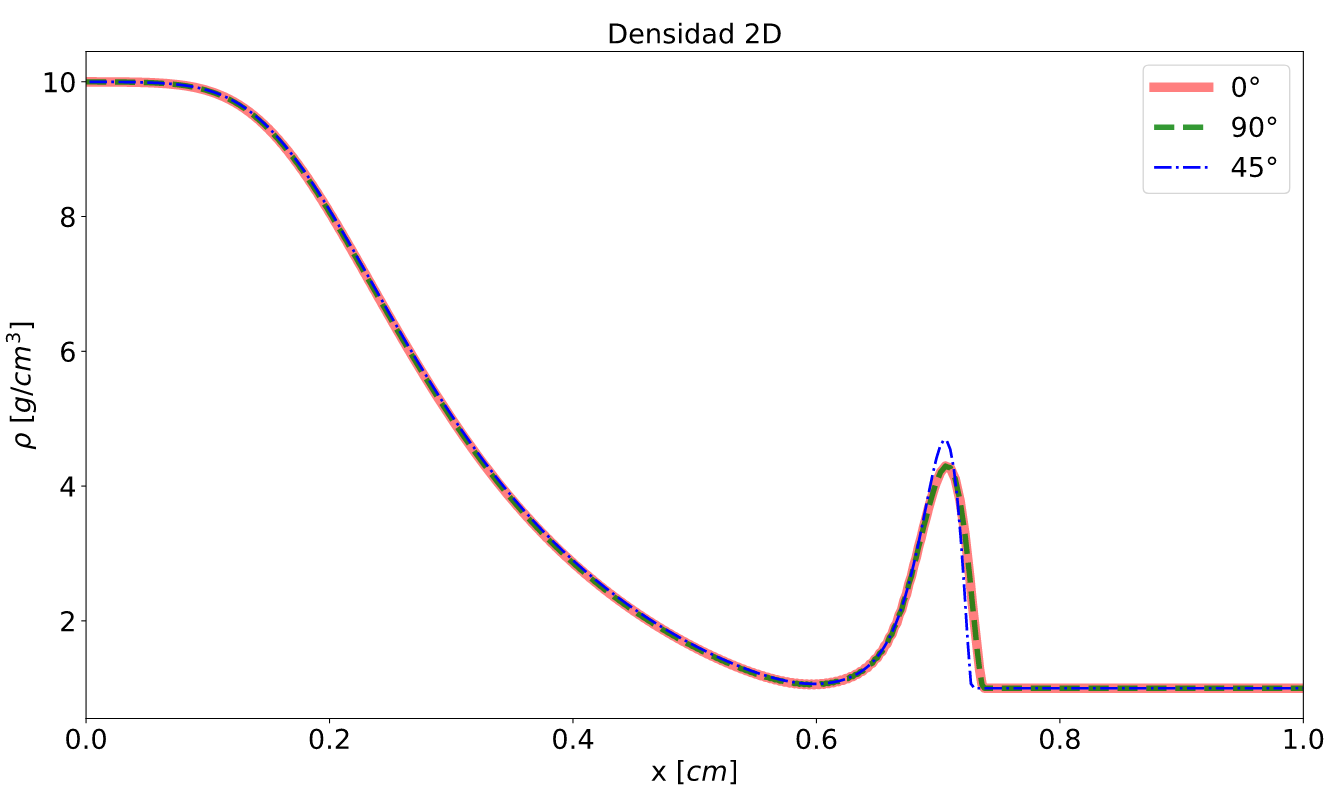
\includegraphics[scale = 0.16]{./Figuras/verificacion_del_codigo/pruebas_2D/combinacion/densidad.png}}
      \subfigure{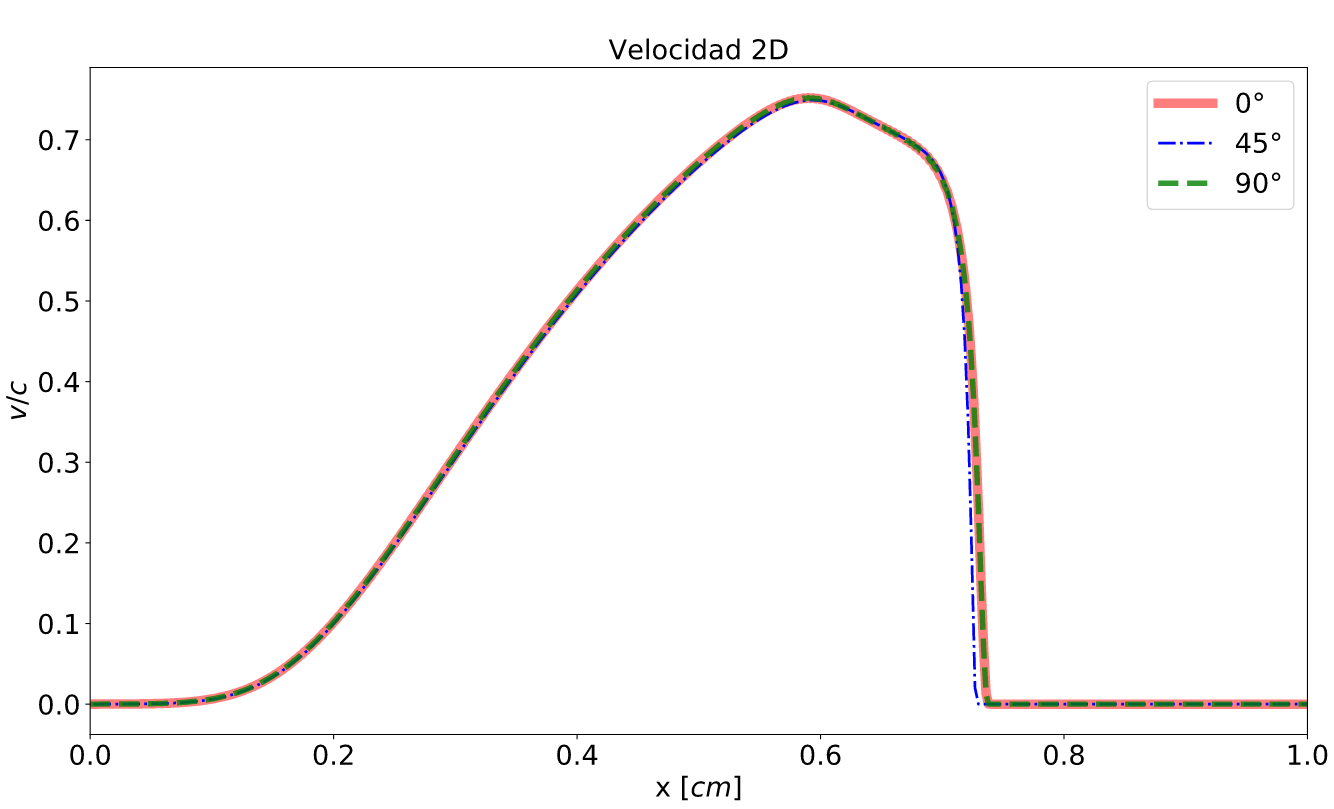
\includegraphics[scale = 0.16]{./Figuras/verificacion_del_codigo/pruebas_2D/combinacion/velocidad.png}}
      \subfigure{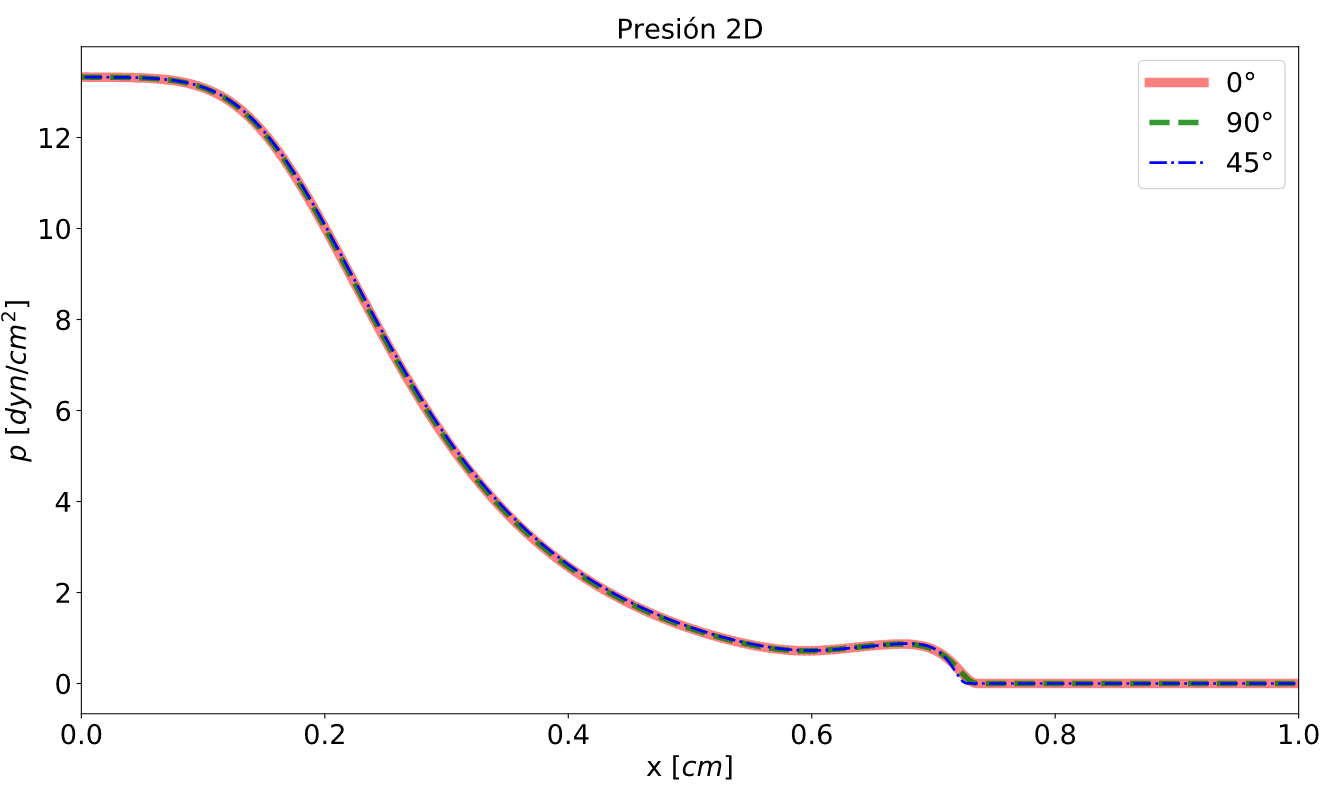
\includegraphics[scale = 0.16]{./Figuras/verificacion_del_codigo/pruebas_2D/combinacion/presion.png}}
    \caption{La figura muestra la comparación que hay entre los distintos perfiles de
    densidad al tiempo $t = 0.4$ s. El panel de arriba a la izquierda muestra el perfil a 0° (línea roja
    sólida), el de arriba a la derecha muestra a 90° (línea verde punteada) y el panel de abajo 
    (línea azul de raya y punto) muestra a 45°.}
    \label{fig:comparacion_perfil_radial}
\end{figure}

En la Figura \ref{fig:comparacion_perfil_mean} se muestra la comparación entre la prueba unidimensional
y la prueba bidimensional, que es la media de los 3 perfiles radiales que se discutieron anteriormente.
El panel de arriba a la izquierda muestra la densidad, el de arriba a la derecha, la velocidad y 
el de abajo la presión. Para ambas pruebas, se mantienen sus valores de 
$\rho = 10 \,  \text{g}/ \text{cm}^3$ y $p = 13.33 \,  \text{dyn}/ \text{cm}^2 $ 
luego, bajan sus valores en $x \approx 0.25$ cm,
mientras que la velocidad, la cual es nula,
asciende. En el punto $x \approx 0.68$ cm la presión alcanza 
$p \approx 2.0\,  \text{dyn}/ \text{cm}^2 $ y la densidad
$\rho \approx 2.0 \,  \text{g}/ \text{cm}^3$, mientras que la velocidad sube a $v \approx 0.75c$
en una dimensión. En 2 dimensiones la densidad baja hasta  $\rho \approx 1.0 \,  \text{g}/ \text{cm}^3$ y
la presión, $p \approx 1.8\,  \text{dyn}/ \text{cm}^2 $ mientras que la velocidad en $x \approx 0.68$ cm
sube a $v \approx 0.8c$ y baja a $v \approx 0.7c$ en $x \approx 0.68$ cm.

\begin{figure}
  \centering
      \subfigure{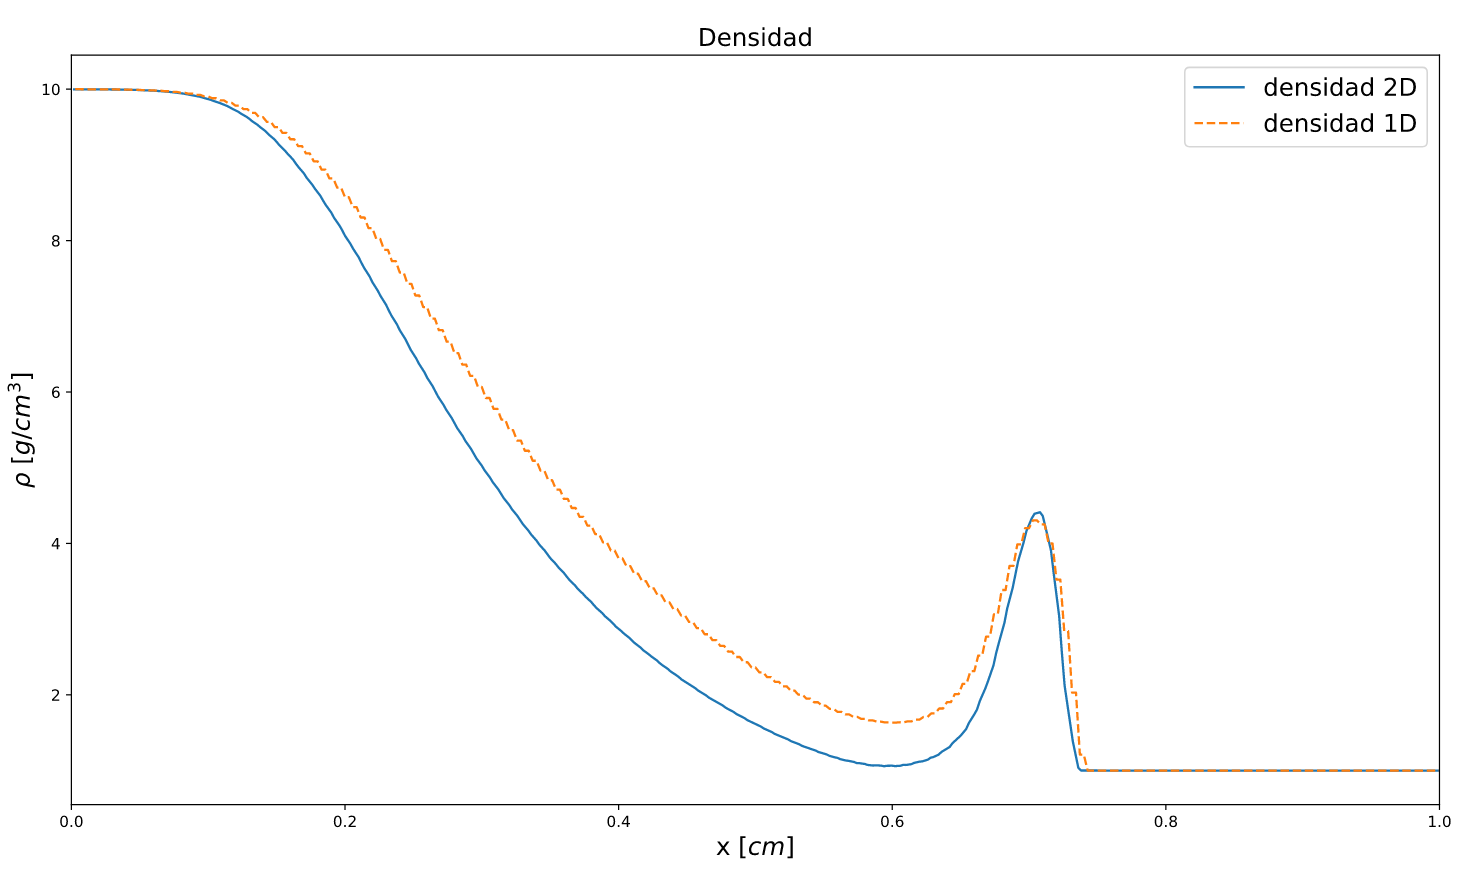
\includegraphics[scale = 0.2]{./Figuras/verificacion_del_codigo/pruebas_2D/mean/densidad.png}}
      \subfigure{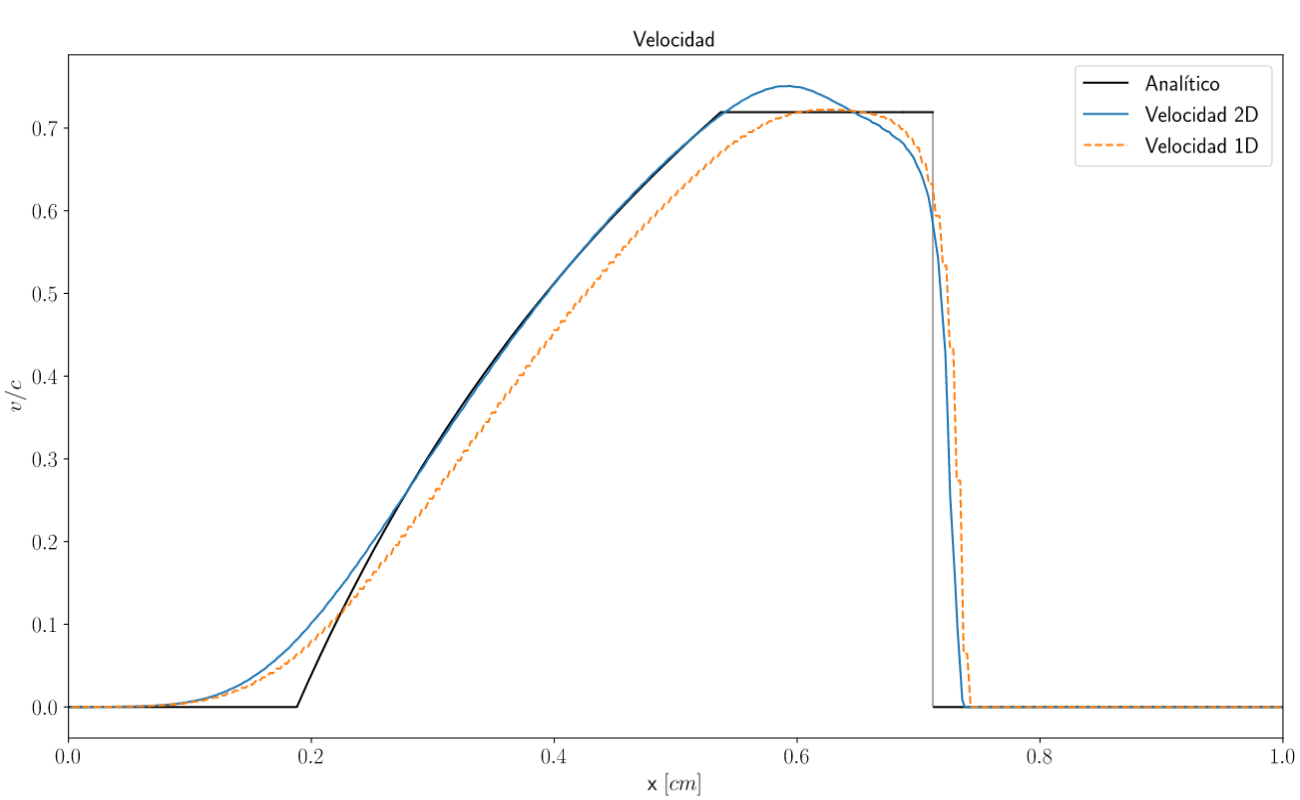
\includegraphics[scale = 0.21]{./Figuras/verificacion_del_codigo/pruebas_2D/mean/velocidad.png}}
      \subfigure{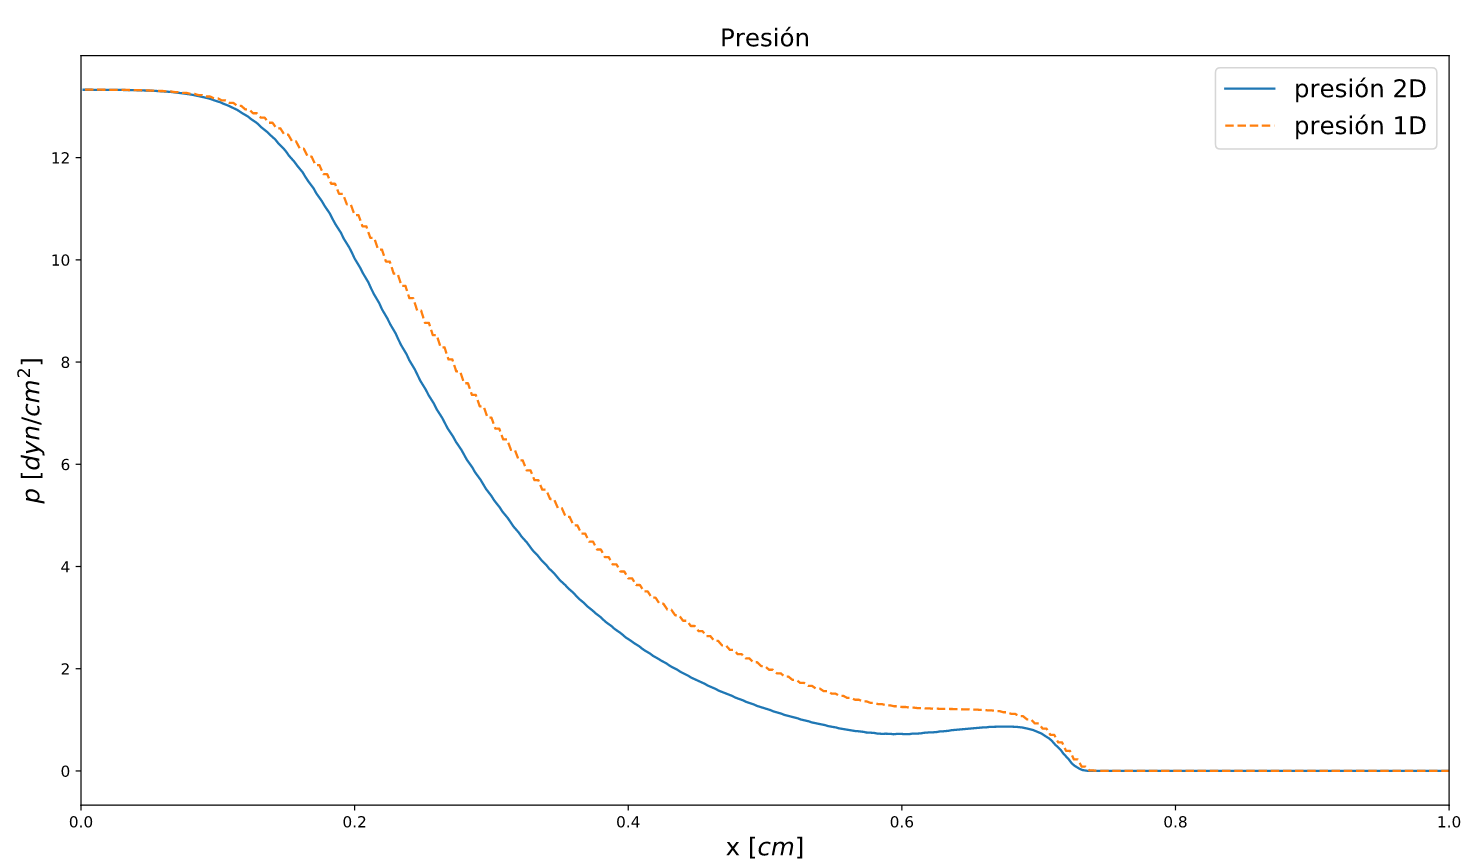
\includegraphics[scale = 0.2]{./Figuras/verificacion_del_codigo/pruebas_2D/mean/presion.png}}
    \caption{Comparación entre la media de los 3 perfiles radiales (línea sólida azul), la 
    la prueba unidimensional (línea de puntos rojos) y la analítica (línea negra sólida)
    .}\label{fig:comparacion_perfil_mean}
\end{figure}

La densidad en 1D y 2D vuelve a subir
en $x \approx 0.69$ cm y llega a $\rho \approx 5 \,  \text{g}/ \text{cm}^3$ y 
se mantiene así hasta el punto $x \approx 0.7$ cm 
donde la densidad, así como la velocidad y presión, descienden sus valores a cero.
Cabe señalar que la mayor diferencia que hay entre la 1D y 2D para la densidad es del 70 \%, mientras que para la 
velocidad es del 238 \% y la de la presión es del 79 \%.
Al comparar los perfiles bidimensionales con el analítico, para la densidad se tiene un error promedio del
13 \%, para la velocidad del 12 \% y para la presión del 16 \% y errores máximos del 156 \%, 19 \% y 119 \%. 
Para el caso unidimensional con el analítico, el error medio para la $\rho$, $v$ y $p$ son 
3 \%,  7\% y  4 \% y error máximo 119 \%, 20 \% y 3 \% respectivamente.
Al no haber tanta diferencia del resultado de los perfiles radiales bidimensionales con 
los perfiles unidimensionales y con el analítico, se puede concluir que el código relativista es válido
en una y dos dimensiones.



% %==============================CAPITULO JET======================================
% %============================================================================


\chapter{Jets relativistas bidimensionales}

En este capítulo se estudiará la evolución de un jet 2D relativista (usando el módulo 2D HLL que se detalla en el capítulo \ref{cap:Verificacion_del_codigo}) a través de medios con distinta densidad. La primera prueba consistirá en estudiar el caso en que el jet atraviesa un medio constante y  comparar los resultados con aquellos de Mignone \emph{et al.} (2005). 
Después, se estudiarán los efectos que un medio que varía en función de la distancia produce en los jets relativistas.
El jet se modelará como un flujo cilíndrico con densidad $\rho_j$, presión $P_j$,  y velocidad $v_j \simeq c$ 
(ver el cuadro \ref{Cuadro: propiedades-jet-comparacion} para más detalles). El índice adiabático será $\Gamma = 5/3$, 
consistente con \citet{MB-HLLC-I}. 
Los cuales en la primera prueba serán constantes y luego variarán en función de x. El medio ambiente, a su vez, se modelará con una densidad y presión en reposo. Un jet de grosor $\Delta y$ será inyectado 
en la frontera $x_{min}$ a la mitad de la altura $y_{max}$ (esto es, desde $\frac{y_{max}-\Delta y}{2}$ hasta 
$\frac{y_{max}+ \Delta y}{2}$). 
El resto de la frontera de $x_{min}$ así como las otras fronteras ($x_{max}$, $y_{min}$, $y_{max}$) tendrán condiciones a la
frontera de \emph{outflow}. 
El dominio espacial será $x, y \in [0,40]\times[0,20]$ con una resolución de 3200x1600 píxeles). 
Cabe señalar que el diámetro del jet será de $\delta y=80$ píxeles. El tiempo de integración total será $t = 100$, y el parámetro de Courant será $\text{Co} = 0.5$.

%====================================TABLE=================================
\begin{table}[htbp]
\begin{center}
\begin{tabular}{|c|c|c|}
\hline 
\textbf{Parámetro} & \textbf{Descripción} & \textbf{valor} \\ 
\hline 
$\rho_{j}$ &  Densidad del jet & 0.1  \\ 
\hline 
$\rho_{a}$ &  Densidad del medio ambiente & 10   \\
\hline 
$P_{j}$ & Presión interna del jet& $0.01 $ \\ 
\hline 
$P_{a}$ &  Presión del medio ambiente & $0.01 $  \\ 
\hline 
$v_{x_{j}}$ & Velocidad interna en el eje x del jet & 0.99 c \\ 
\hline 
$v_{y_{j}}$ & Velocidad interna en el eje y del jet & 0.0 c \\ 
\hline 
$v_{x_{a}}$ & Velocidad en el eje x del medio ambiente & 0.0 c \\
\hline 
$v_{y_{a}}$ & Velocidad en el eje y del medio ambiente & 0.0 c \\ 
\hline 
Co & Número de Courant & 0.5 \\ 
\hline 
\end{tabular}
\caption{\label{Cuadro: propiedades-jet-comparacion} Valores iniciales de la densidad ,
velocidad  y presión  en el jet ($\rho_j$, $v_{xj}$, $v_{yj}$, $p_j$) en unidades adimensionales y 
del medio ambiente ($\rho_a$, $v_{xa}$, $v_{ya}$, $p_{a}$). El jet será relativista, con un dominio 
$x, y \in [0,40]\times[0,20]$ y un índice adiabático $\Gamma = 5/3$.}
\end{center}
\end{table}

\section{Jet 2D RHD en un medio ambiente constante} \label{sec:jet_ambiente_constante}

Para el caso en que el jet, \Selenecor{el cual tiene una densidad}{de densidad} $\rho_j = 0.1$, una velocidad que solo cambia en el eje x de $v_{x_{j}} = 0.99 \, c$, una presión $p_j = 0.01$ que se mueve a través de un medio en reposo y \Selenecor{con densidad}{una densidad} y presión constante, en el cual 
$\rho_a = 0.1 $ y $P_a = 0.01$ es consistente con los valores que \citet{MB-HLLC-I} utilizó. 
En la Figura \ref{fig:evolucion_temporal_del_jet} se muestra la evolución del jet a 
través del medio constante en mapas de densidad a los tiempos $t = 1$ (arriba a la izquierda), $t = 10$ (arriba a la derecha), $t = 20$ (abajo a la izquierda) y $t = 40$ (abajo a la derecha).
En el tiempo $t = 1$, el jet apenas es visible y solo llega a $x \approx 1$. 
Cuando $t = 10$ la longitud del jet llega  a $x \approx 6$ de longitud, las ondas de colimación, se observan a longitudes de y=10 y llegan a $x \approx 4$. Los isocontornos blancos delimitan el material menos denso del jet. 
El capullo se expande a 5 unidades de longitud, mientras que de ancho alcanza 4 unidades.
Para el tiempo $t = 20$, el jet se expande a 
$x \approx 10$ unidades de longitud. El capullo mide 4 unidades de ancho a partir de parte $y > 10$, 
las ondas de colimación no cambian, mantienen su posición en $x \approx 4$ a lo longitud del eje $y = 10$, el jet se incrementa a 7 unidades de longitud. Para el tiempo $t = 40$, el jet incrementa su tamaño a $x \approx 21$ de longitud. 
El capullo sobrepasa las 10 unidades de ancho, es decir, sale de nuestro dominio. Las ondas de colimación siguen manteniendo el mismo tamaño en $x \approx 4$ y el capullo sobresale de nuestro dominio. Podemos notar que el capullo está compuesto de materia poco densa que el jet, donde alcanza valores mínimos de $\rho \approx 0.05 $ y máximos de $\rho  \approx 20$ en la
parte externa del capullo. Cabe destacar que el jet conserva el mismo ancho y que la longitud del capullo crece 
en la misma proporción a la longitud del jet.

El jet del estudio de  \citet{MB-HLLC-I} utiliza un jet relativista con simetría axial en 
coordenadas cilíndricas,  en este modelo, se usaron coordenadas cartesianas. 
Ellos usan una ecuación de estado ideal con $\Gamma = 5/3$, el dominio es 
$0 \leqslant r \leqslant 12$ y $0 \leqslant z \leqslant 35$ con una malla de 240 x 700. Las condiciones de
frontera son \emph{outflow} en todas su frontera, excepto donde está la eyección. El número de Courant que
usa es 0.5 y el tiempo de integración es hasta $t = 80$. Los valores del jet y su medio ambiente son los
mismos que la del Cuadro \ref{Cuadro: propiedades-jet-comparacion}. El jet que se usó en esta tesis tiene las
misma ecuación de estado que se usó en \citet{MB-HLLC-I}, se integró en el mismo tiempo, y aunque son distintos sistemas de coordenadas, tienen el mismo dominio, así como las mismas condiciones de frontera. Se diferencian únicamente, por la resolución, ya que el jet de este estudio tiene aproximadamente 3 veces más, la resolución usada en \citet{MB-HLLC-I}.

\begin{figure}
  \centering
  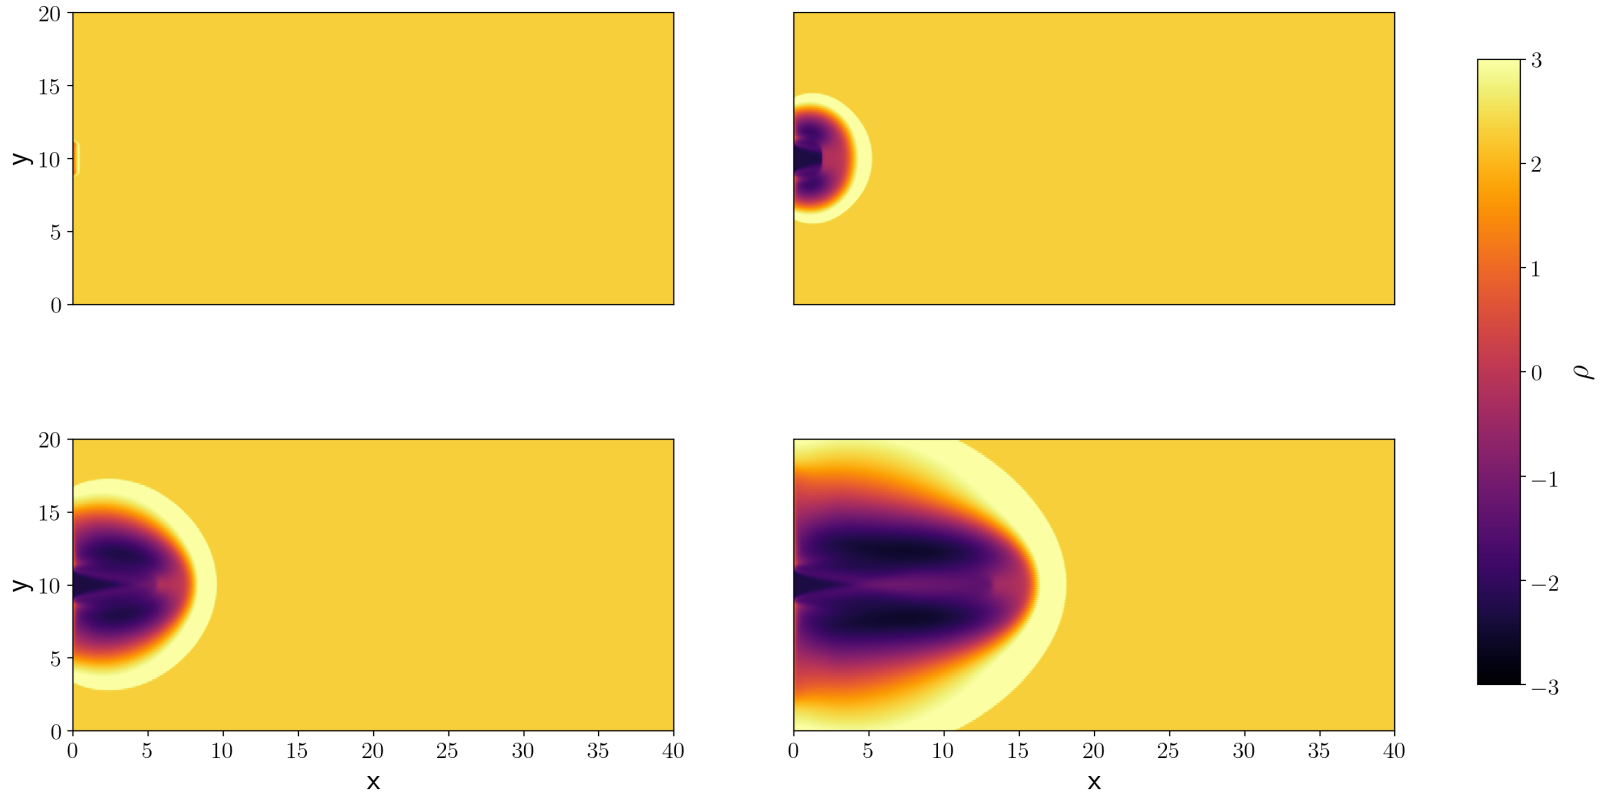
\includegraphics[width=1\textwidth]{./Figuras/jet/evolucion/evolucion.png}
    \caption{Mapas de densidad en los que se muestra la evolución del jet relativista 
    con los valores del Cuadro 
    \ref{Cuadro: propiedades-jet-comparacion}. El panel de arriba a la izquierda muestra al 
    tiempo t = 1, el de arriba a la derecha muestra al tiempo t = 10, 
    el de abajo a la izquierda muestra al tiempo t = 20 y el de abajo al tiempo t = 40.
    También se emplearon isocontornos (líneas punteadas) que se componen de 5 niveles. En los 
    cuales el nivel más bajo, que es blanco, corresponde a $\rho \approx 0.13$, blanco ligeramente grisáceo 
    para $\rho \approx 0.36$,
    gris para $\rho \approx 1$, gris oscuro para $\rho  \approx 2.7$ y el nivel más alto, que es negro, 
    corresponde a $\rho \approx 7.3$.}
    \label{fig:evolucion_temporal_del_jet}
\end{figure}

En la Figura \ref{fig:Decaimiento_constante_densidad_jet} se muestra la comparación entre los perfiles de 
densidad a $y = 10$
del jet al tiempo t = 0, donde no se muestra una onda; a t = 5 donde la onda se localiza en $x \approx 2$; 
a t = 20, la onda se localiza a $x \approx 8$; y  t = 50, donde la onda se localiza en $x \approx 20$. 
El panel de arriba a la izquierda muestra la densidad, en donde
podemos observar que para $x \approx 2, 8, 20$,  la densidad alcanza un valor máximo de 
$\rho  \approx 33$.
En el panel de arriba a la derecha se muestra la velocidad, donde se puede ver que el jet mantiene una velocidad 
$v \approx 0.9 \, c$ y decae en $x \approx 17.5$ para llegar a $v \approx 0 $ en  $x \approx 21$. 
En el panel de abajo a la
izquierda se muestra la presión, la cual se puede observar que es parecido a la gráfica de la 
densidad, ya que mantiene sus máximos en los puntos $x \approx 2, 8, 20$, pero también se observa que conforme avanza el
tiempo los picos empiezan a decrecer, ya que para $t = 5, \, p \approx 1.6 $; 
para $t = 20, \, p \approx 1.49$ y para 
$t = 50, \, p  \approx 1.3$. Para el panel de abajo a la derecha, se hizo la misma comparación que el panel 
de la densidad, solo que esta vez se compararon  distintas resoluciones: baja resolución "LD" (con 1600 píxeles en el eje X y 800 en el eje Y) 
y alta resolución "HD" (3200x1600), con lo que se puede observar que 
para mayor resolución el jet se vuelve ligeramente más rápido. En este panel se puede notar que
los picos están desfasados conforme avanza el tiempo. Los efectos de la resolución son despreciables ya 
que la mayor diferencia, debida a la resolución, en la magnitud de los picos es relativamente pequeña (menor a 5\%). \Selene{Esta}, se presenta a t=50 y corresponde a $\frac{\rho_{alta} - \rho_{baja}}{\rho_{alta}} \approx 0.04$.


\begin{figure}
  \centering
  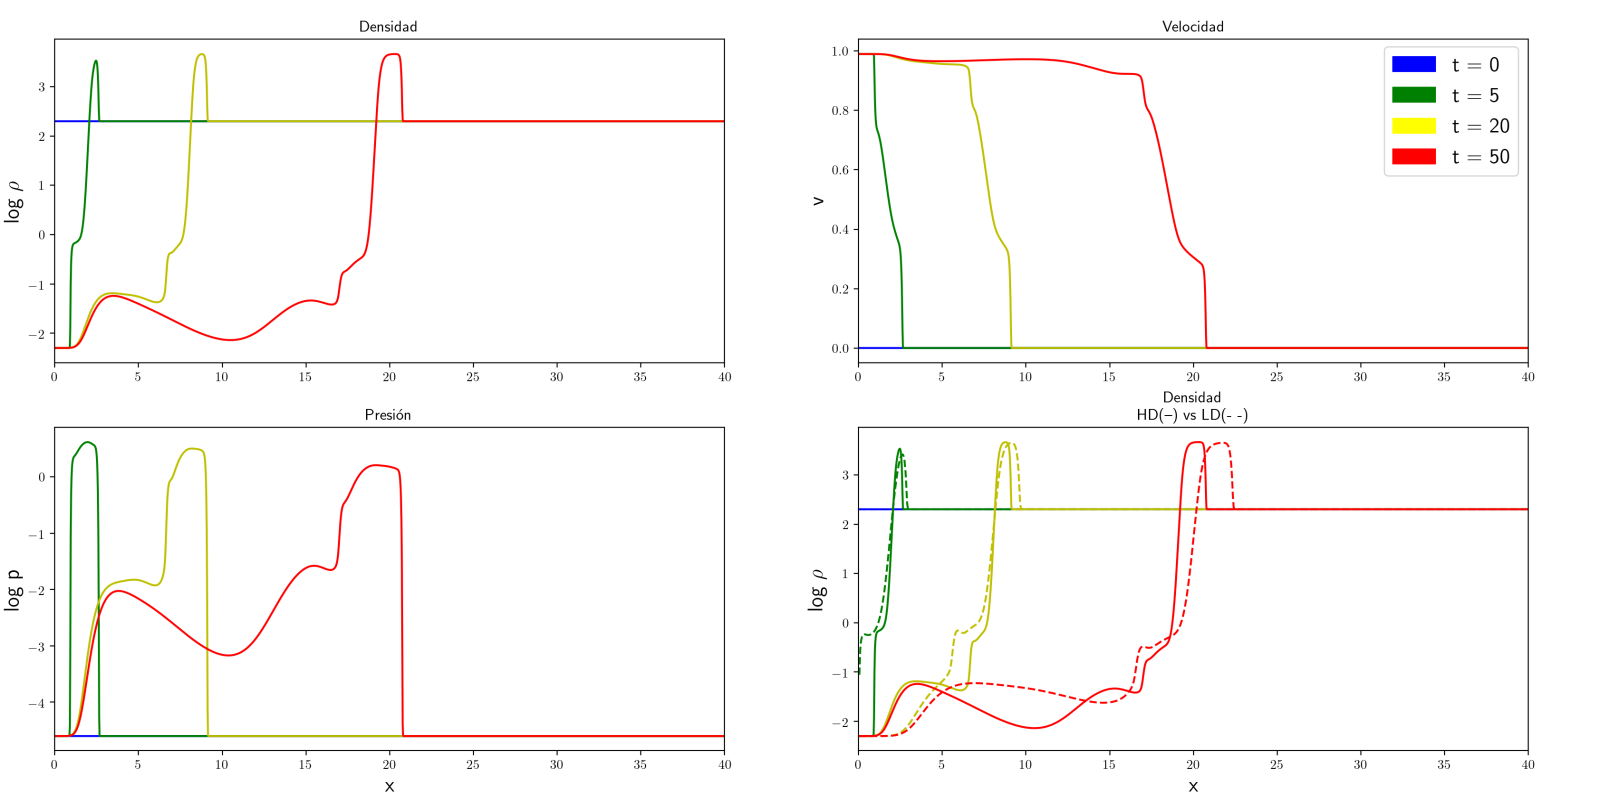
\includegraphics[width = 1.0\textwidth]{./Figuras/jet/perfiles/perfiles_constantes.png}
  \caption{Perfiles de densidad, velocidad, presión y distintas resoluciones, similar a la Figura 
  \ref{fig:comparacion_perfil_radial} a tiempos t=0, 5,20, 50.
  El perfil es de $y = 10$.
  La densidad (arriba a la izquierda), velocidad (arriba a la derecha), la presión (abajo a la izquierda). 
  En el panel de abajo a la derecha se comparan la densidad usando 2 distintas resoluciones. La de alta resolución 
  (HD)
  es de 3200x1600 píxeles y la de baja resolución (LD) es de 1600x800 píxeles.}\label{fig:Decaimiento_constante_densidad_jet}
\end{figure}

En la Figura \ref{fig:comparacion_temporal_del_jet}  \Selenecor{se muestra}{se muestran} los resultados obtenidos en baja 
(1600x800 píxeles) y alta (3200x1600) resolución, a 
las mismas escalas de densidad, en comparación con los resultados de \citet{MB-HLLC-I}.
La Figura muestra de izquierda a derecha las gráficas de \citet{MB-HLLC-I} (izquierda), el modelo con baja resolución 
(medio) y el modelo con alta resolución (derecha). Los paneles de arriba muestran al tiempo t = 40, mientras que los 
de abajo al tiempo t = 80.
Al enfocarse en los paneles de arriba, al tiempo t = 40, se puede observar que el jet de estudio de \citet{MB-HLLC-I} tiene un largo 
de $x \approx 18$ unidades, mientras que el de baja resolución tiene un largo de 19 unidades y 
el jet de alta densidad  tiene un largo de 19 unidades, por lo que podemos observar un error del 5 \% 
con baja resolución y del 0 \% con el de alta resolución. El capullo está compuesto de material de alta densidad 
que rodea al jet, su ancho se mantiene en aproximadamente 5 unidades.
Los choques de colimación son más grandes en el estudio de \citet{MB-HLLC-I}
que en el de baja resolución, 
dado que se localizan en $x \approx 10$ y $x \approx 5$ respectivamente, una diferencia del 50 \%. 
Los choques de alta resolución se localizan en $x \approx 4$  lo que muestra una diferencia de más del 
60 \% con el estudio de \citet{MB-HLLC-I}.
Se observa también que el capullo de baja resolución mide más de 11 unidades de ancho para $y > 10$, 
mientras que para la resolución alta mide 9 unidades, lo que nos da un error, solo para la resolución alta del 33 \%.
Tanto en el capullo de baja resolución como en el de alta resolución no se muestran turbulencias 
como en el estudio de \citet{MB-HLLC-I}, lo que da a entender  que el código que fue desarrollado para esta tesis 
es más viscoso.
Para los paneles de abajo, el tiempo ahora es t = 80, se puede observar que el capullo sobresale del dominio para los 
3 casos que estamos comparando. Las ondas de colimación para alta como baja resolución están en $x = 3$ mientras que las de \citet{MB-HLLC-I} se siguen manteniendo en $x = 6$, lo que nos sigue dando un error 
del 50 \%, por lo que estas no dependen del tiempo. 
El jet para el estudio de \citet{MB-HLLC-I} mide $x \approx 35$ de largo, para el jet de resolución baja mide $x \approx 32$ unidades y 
para el de resolución alta $x \approx 31$ unidades, lo que nos da un error del 9 \% para resolución baja y con el 
de resolución alta un error del 11 \%.
Otra diferencia fue que el jet de 
alta resolución está más comprimido, ya que tiene un grosor aproximado de 1.0 unidades, 
mientras que el de baja resolución tiene una resolución aproximada de 1.4 unidades, 
aunque no está tan comprimido como el jet mostrado en el estudio de \citet{MB-HLLC-I}. así también, no podemos encontrar, tanto para baja como 
alta resolución, las turbulencias generadas en el jet de \citet{MB-HLLC-I}, pero también no se pueden comparar las densidades del 
mismo debido a que no presenta los valores.

\begin{figure}
  \centering
  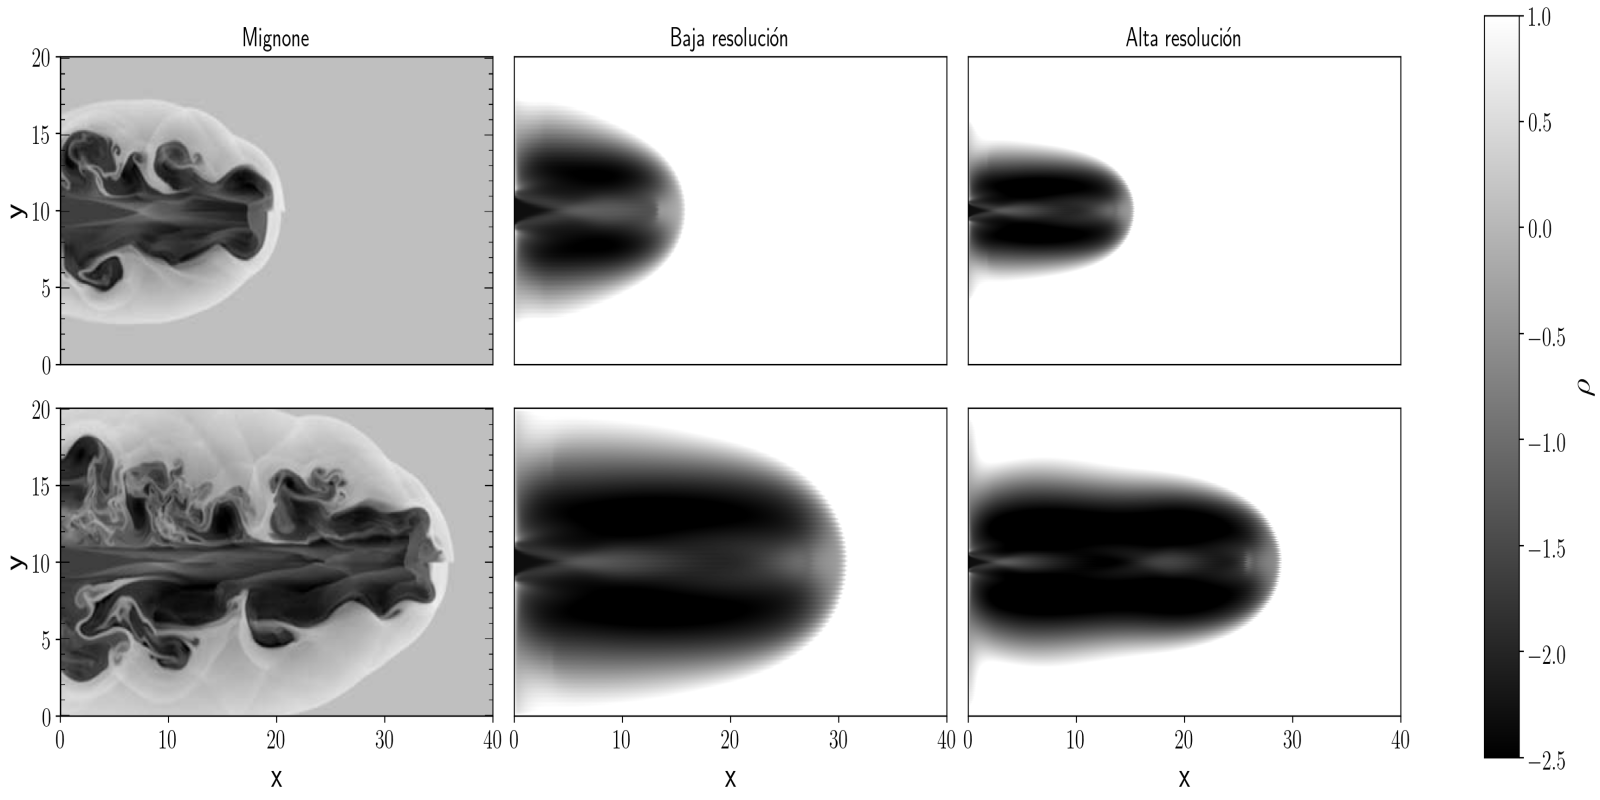
\includegraphics[width=1\textwidth]{./Figuras/jet/comparacion/multiple_comparation.png}
    \caption{Mapas de densidad en los que se compara el jet relativista con los valores del Cuadro 
    \ref{Cuadro: propiedades-jet-comparacion}. La Figura está dividida en 3 columnas. La de la izquierda muestra
    el estudio de \citet{MB-HLLC-I}, la de en medio el jet a baja resolución (1600x800 píxeles), y la de la derecha el jet a alta 
    resolución (3200x1600 píxeles).
    }\label{fig:comparacion_temporal_del_jet}
\end{figure}


\section{Jet 2D RHD en un medio ambiente variable} \label{sec:jet_ambiente_variable}
Esta sección estudia los efectos que un medio que varía en función de la distancia, $\rho = \rho(x)$, 
produce en un jet. La densidad del medio ambiente variará en función del eje, es decir, se modelará como:

\begin{equation}
  \rho(x) \varpropto \frac{1}{x} \,\,\,\,\,\,\,\,\, \text{y} \,\,\,\,\,\,\,\,\, \rho(x) \varpropto \frac{1}{x^2}
\end{equation}
donde $\rho_a$ es el valor mostrado en el Cuadro \ref{Cuadro: propiedades-jet-comparacion}.

La Figura \ref{fig:Decaimiento_lineal_densidad_jet} muestra los perfiles de densidad, velocidad y presión, es decir, solo mostrará los valores que estén sobre $y = 10$ {para el caso cuando $\rho \varpropto \frac{1}{x}$}. En el panel de arriba 
a la izquierda  muestra la densidad. El de arriba a la derecha, la velocidad. El de abajo a la izquierda la presión y 
el de abajo a la derecha muestra la comparación entre
uno de mayor resolución con uno de baja resolución. Al tiempo t = 0, al no haber una inyección del jet, únicamente la densidad 
decae como $\frac{1}{x}$. Al tiempo t = 5, la densidad, en x = 3 tiene un máximo local que llega a 
$\rho  \approx 33$, en t = 20, el pico se sitúa en $x \approx 12$ con un máximo de 
$\rho  \approx 16.5$ y para el 
tiempo t = 50, el pico se sitúa en $x \approx 33$ con $\rho  \approx 3.6$ por lo que los máximos disminuyen en función de la 
densidad del medio ambiente.
La velocidad tiene un máximo en $x \approx 0.2$, donde alcanza  $v \approx 0.6$. Para los tiempos t = 20, 50 ya no 
presenta máximos, sino que decae rápidamente en las posiciones $x \approx 8, \, 25$ respectivamente.
La presión tiene un valor máximo al tiempo t = 5 con $p \approx 1.64$, aunque si un cambio menos abrupto en $x = 3$. 
En los tiempos t = 20, 50 los máximos globales se sitúan en $x \approx 12$ y en $x \approx 33$ 
con $p \approx  1$ y $p  \approx 0.6$ respectivamente.
En el panel inferior derecho, al comparar la densidad en resoluciones de 3200x1600 y 1600x800,
notamos que a diferencia del medio constante, no hay un desfase tan grande.  Los efectos de la resolución en este caso 
también son pequeños. Lo anterior se debe a que la mayor diferencia, debida a la resolución, 
en la magnitud de los picos es menor a 10\% ($\frac{\rho_{alta} - \rho_{baja}}{\rho_{alta}} \approx 0.04$ a t=50). 

\begin{figure}
  \centering
  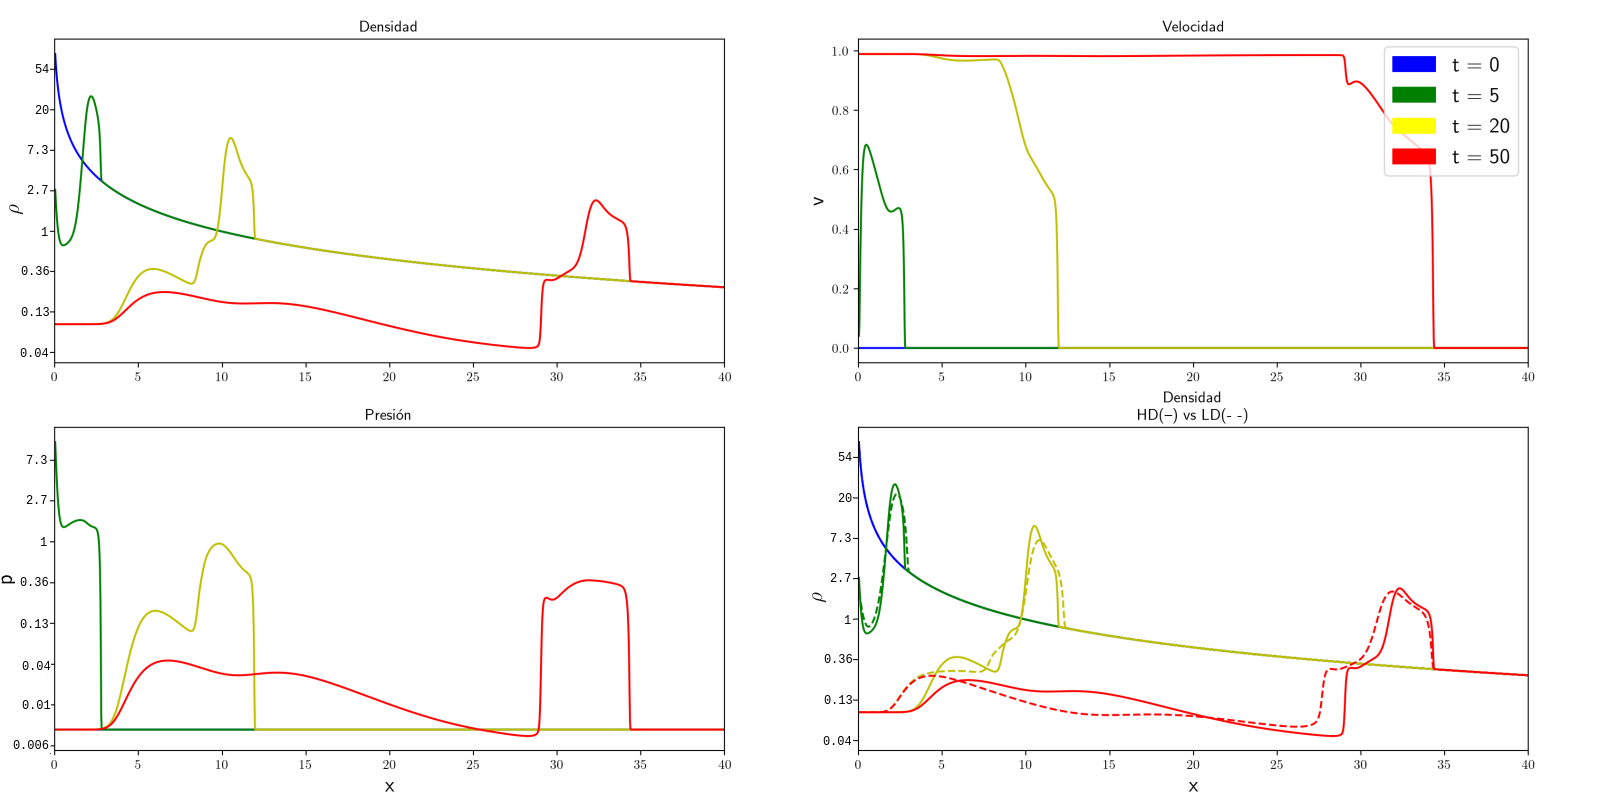
\includegraphics[width = 1.0\textwidth]{./Figuras/jet/perfiles/perfiles_lineales.png}
  \caption{Perfiles de densidad, velocidad, presión y distintas resoluciones, similar a la Figura 
  \ref{fig:comparacion_perfil_radial} para un perfil de densidad que varía en función de la distancia como
  $\rho \varpropto \frac{1}{x}$ a tiempos t=0, 5,20, 50.
  El perfil es de $y = 10$.
  La densidad (arriba a la izquierda), velocidad (arriba a la derecha), la presión (abajo a la izquierda). 
  En el panel de abajo a la derecha se comparan la densidad usando 2 distintas resoluciones. La de alta resolución
  es de 3200x1600 y la de baja resolución es de 1600x800.}\label{fig:Decaimiento_lineal_densidad_jet}
\end{figure}

En la Figura \ref{fig:Decaimiento_cuadratico_densidad_jet} se muestra la densidad de medio ambiente que decae como $\rho \varpropto \frac{1}{x^2}$. Aquí podemos ver que los  picos de la densidad están en x = 3, 10, 33 con  la densidad $\rho \approx 54, \,  10, \,  7.3$, respectivamente. En la velocidad podemos observar el frente de choque de la onda que se ubican en $x \approx 3, \, 13, \, 37$ con los valores de velocidad $v \approx 0.42, \, 0.58, \, 0.60$ respectivamente. Para más detalles véase el Cuadro \ref{Cuadro:valores_frente_choque}.
En el caso de la presión, al tiempo t = 5, desciende rápidamente en $x \approx 0.5$ de $p  \approx 10$ a $p  \approx 2.7$. En el tiempo t = 20, la presión tiene un valor máximo en $x \approx 10$, donde mantiene un valor de $p \approx e^2 \approx 7.3$. Para el tiempo t = 50 la presión desciende exponencialmente del punto $x \approx 28$ donde $p \approx e^{-5} \approx 0.006$. Al comparar las resoluciones de 1600x800 con la de 800x400 se vuelve a ver un desfase. Los efectos de la resolución en este caso dejan deben ser tomados en cuenta. Lo anterior se debe a que la mayor diferencia, debida a la resolución, en la magnitud de los picos es mayor al 60\% ($\frac{\rho_{alta} - \rho_{baja}}{\rho_{alta}} \approx 0.63$ a t=50). Por ello, si se deseará estudiar un jet relativista a través de un medio que disminuye como $1/x^2$, o $1/r^2$ es necesario hacer estudios de convergencia para determinar la resolución necesaria para que no influya en los resultados. 

\begin{figure}
  \centering
  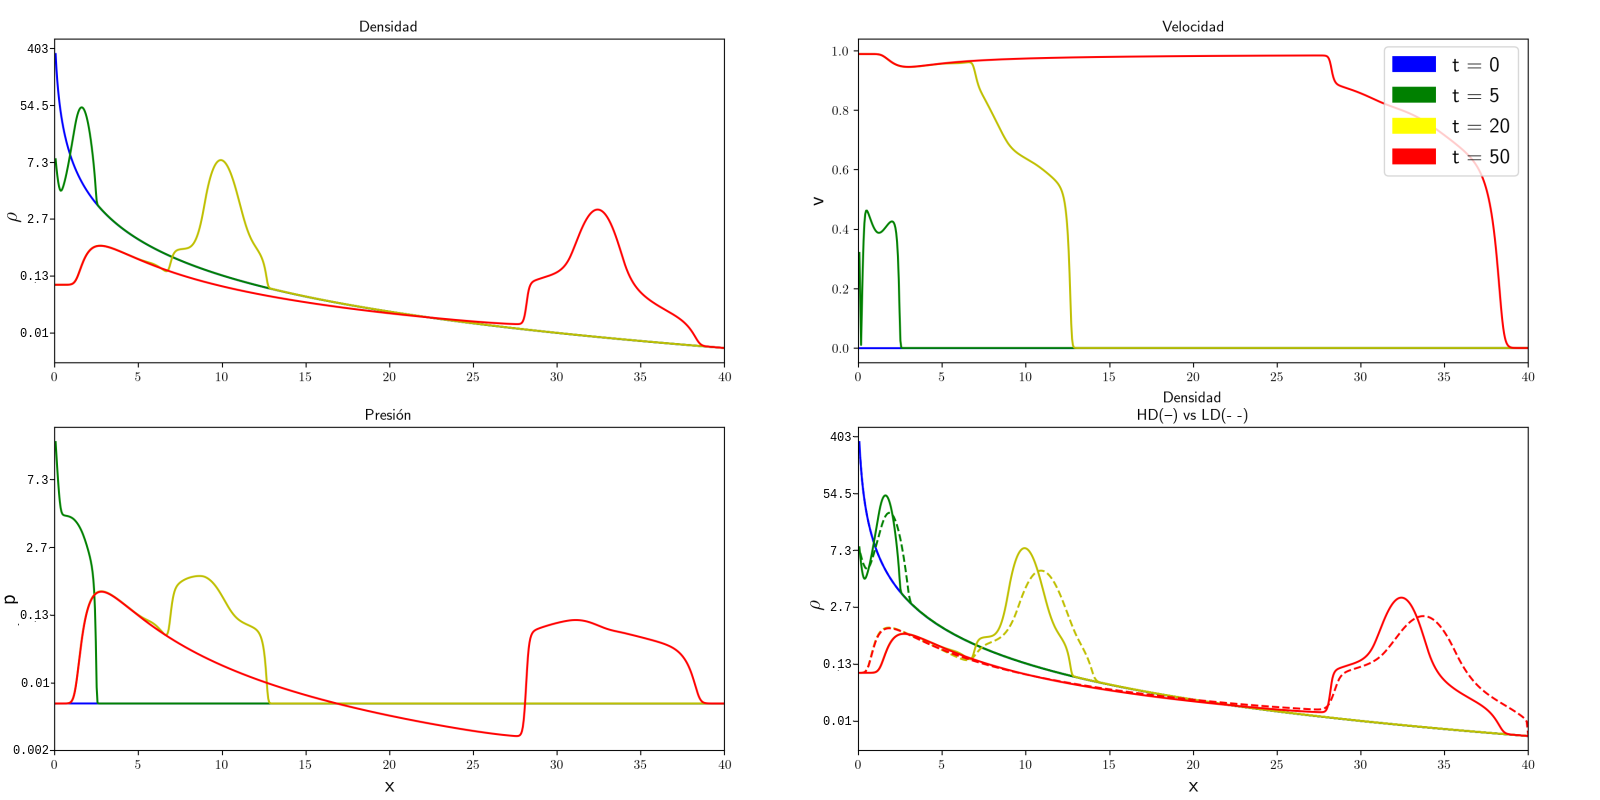
\includegraphics[width = 1.0\textwidth]{./Figuras/jet/perfiles/perfiles_cuadraticos.png}
  \caption{Perfiles de densidad, velocidad, presión y distintas resoluciones, similar a la Figura 
  \ref{fig:comparacion_perfil_radial} para un perfil de densidad que varía en función de la distancia como
  $\rho \varpropto \frac{1}{x^2}$ a tiempos t = 0, 5,20, 50.
  El perfil es de $y = 10$.
  La densidad (arriba a la izquierda), velocidad (arriba a la derecha), la presión (abajo a la izquierda). 
  En el panel de abajo a la derecha se comparan la densidad usando 2 distintas resoluciones. La de alta resolución
  es de 3200x1600 y la de baja resolución es de 1600x800.}\label{fig:Decaimiento_cuadratico_densidad_jet}
\end{figure}

En resumen, los picos de la densidad y presión 
son en general más pequeños que los mostrados en donde la densidad del medio es constante, pero también recorren mayor 
distancia que los anteriormente mencionados. En cambio, para el caso en que la densidad decae como $\frac{1}{x^2}$, los picos son mayores, pero recorren menos distancia que el medio anteriormente mencionado.


\begin{table}[htbp]
  \begin{center}
  \begin{tabular}{|c|c|c|c|c|c|c|c|c|c|c|c|c|}
    \hline 
    & \multicolumn{4}{|c|}{$\rho = \rho_a$} & \multicolumn{4}{|c|}{$\rho_a \propto x^{-1}$} & \multicolumn{4}{|c|}{$\rho_a \propto x^{-2}$}\\
    \hline
    t & $x_{\text{fch}}$ & $\rho_{\text{fch}}$ & $p_{\text{fch}}$ & $v_{\text{fch}}$ & $x_{\text{fch}}$ & 
    $\rho_{\text{fch}}$ & $p_{\text{fch}}$ & $v_{\text{fch}}$ & $x_{\text{fch}}$ & $\rho_{\text{fch}}$ & $p_{\text{fch}}$ & 
    $v_{\text{fch}}$ \\
    \hline
     5 & 3  & 3.5 & 0.6 & 0.38    &  3  & 3.5 &  0.5  & 0.4     & 3  & 4   & 0.8  & 0.42 \\
    \hline
    20 & 9  & 3.5 & 0.6 & 0.4    &  12 & 2.6 &   0   & 0.55    & 13 & 2   & -1.8 & 0.5 \\
    \hline
    50 & 21 & 3.5 & 0.5 & 0.6    &  34 & 1.1 & -0.5  & 0.64     & 37 & 1.8 & -2.0 & 0.64 \\
    \hline

  \end{tabular}
  \caption{\label{Cuadro:valores_frente_choque} Valores de densidad, presión y velocidad que se muestran en el frente
  de choque de la onda del jet. Los valores obtenidos fueron tomados de las Figura \ref{fig:Decaimiento_constante_densidad_jet},
  \ref{fig:Decaimiento_lineal_densidad_jet} y \ref{fig:Decaimiento_cuadratico_densidad_jet}}
  \end{center}
  \end{table}

Conforme disminuye más rápidamente en función de la distancia \emph{x}, 
se vuelve más rápido. En la Figura \ref{fig:perfiles_comparacion_jet} se muestra la comparación que hay cuando la densidad del medio ambiente cambia constantemente ($\rho \varpropto \rho_a$), cuando varía inversamente lineal ($\rho \varpropto x^{-1}$) y cuando varía inversamente cuadrático ($\rho \varpropto x^{-2}$) al tiempo $t = 50$. Las líneas punteadas muestran los exponentes intermedios entre los valores de 0, 1 y 2 en pasos de 0.2, es decir, la densidad del medio ambiente descenderá como $x^0, \, x^{-0.2}, \, . . . \,  ,x^{-0.8} , \, x^{-1}  , \, x^{-1.2}, \, . . . \,  , x^{-2}$. El primer valor máximo que acentúa más en el decaimiento inversamente cuadrático que se localiza en $x \approx 2$ y tiene un valor $\rho \approx 0.6$. Mientras para el decaimiento inversamente lineal se localiza en $x \approx 3$ y su valor es $\rho  \approx  0.3$. Para el caso constante, no remarca un máximo en especial. El segundo valor máximo, para el caso constante, se localiza en $x \approx 20$ y alcanza $\rho  \approx 33$, conforme se aumente el exponente, el valor máximo se desplaza, así como su disminución de la densidad, ya que para el caso inversamente lineal el máximo se localiza en $x \approx 32$ con $\rho \approx 1$ y para el caso inversamente cuadrático el valor máximo se localizó en $x \approx 34$ con $\rho \approx 0.36 $.  Podemos observar que el primer valor máximo de la gráfica, el medio que varía como $x^{-2}$ tiene un valor mayor que el del medio constante, mientras que para el segundo valor máximo se invierte y el medio constante tiene un valor mayor que el del medio que varía como $x^{-2}$. La velocidad de la onda aumenta un 60 \% para medio inversamente lineal en correspondencia con el medio constante y un 6 \% para el medio inversamente cuadrático en correspondencia con el inversamente lineal.  

\begin{figure}
  \centering
    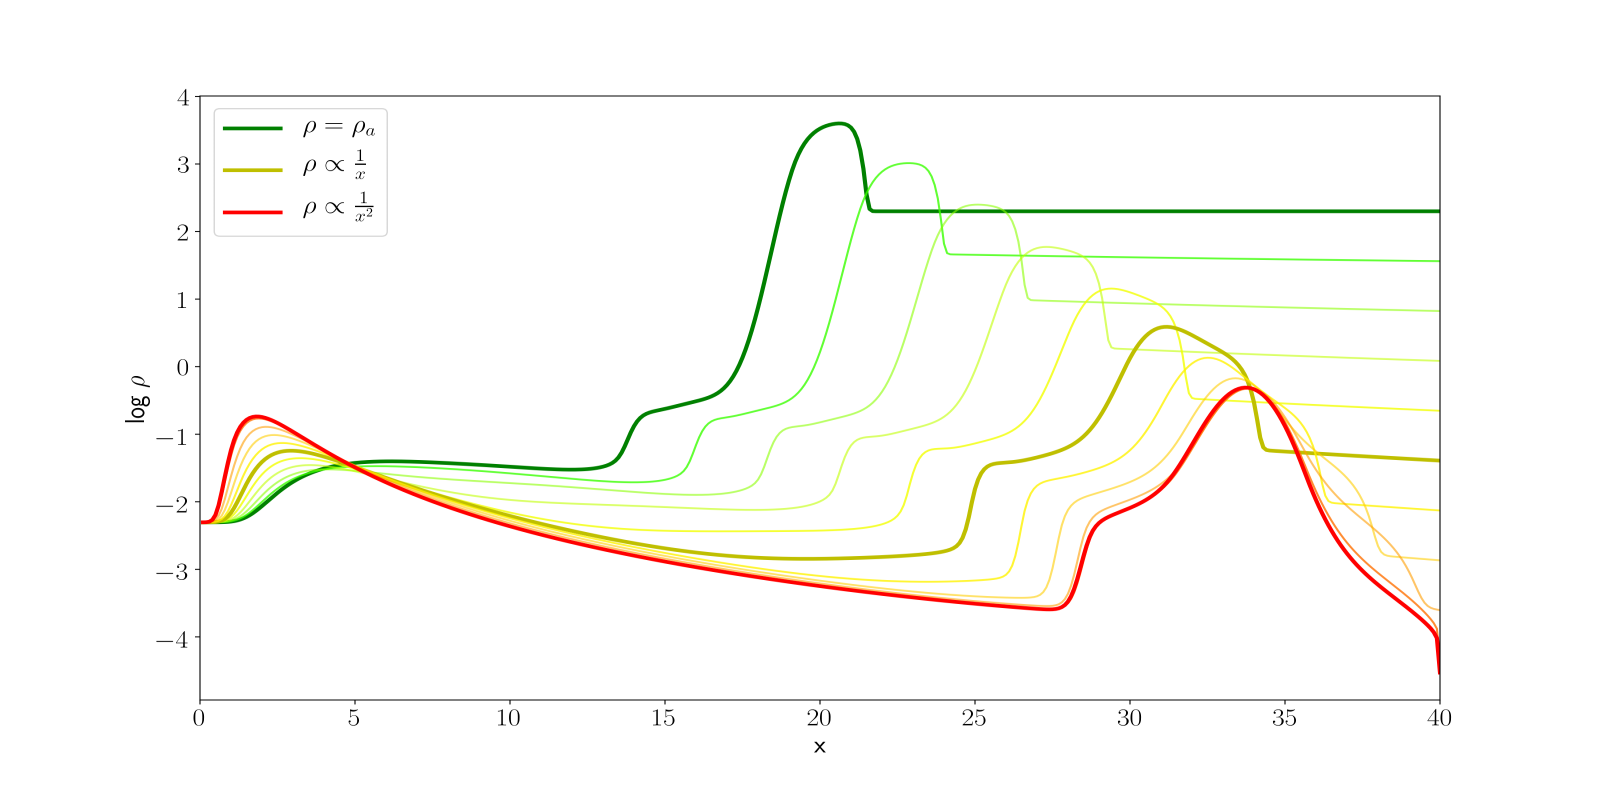
\includegraphics[width=1\textwidth]{./Figuras/jet/perfiles/densidades_comparacion.png}
  \caption{Gráfica de comparación de la posición contra el logaritmo de la densidad 
  donde el medio ambiente es constante $\rho \varpropto k$ (verde), varía inversamente lineal
  $\rho \varpropto x^{-1}$ (amarillo) y varía inversamente cuadrático $\rho \varpropto x^{-2}$ (rojo)
  al tiempo t = 50.  Las líneas punteadas muestran los valores exponenciales entre 0 y 1 y entre 1 y 2,
  es decir, que la densidad descenderá como $x^0, \, x^{-0.2}, \, . . . \,  ,x^{-0.8} , \, x^{-1}  , \, x^{-1.2}
  , \, . . . \,  , x^{-2}$.}\label{fig:perfiles_comparacion_jet}
\end{figure}

%----------------------------------------------------------------------------------------------
\chapter{Conclusiones}
%----------------------------------------------------------------------------------------------
El objetivo principal de esta tesis fue construir un código numérico hidrodinámico que fuera tanto newtoniano como relativista utilizando distintos métodos numéricos de Riemann. Para verificar que el código funcionaba correctamente, dicho código debía ser capaz de reproducir pruebas numéricas cuya solución ya era conocida previamente (ya fuera por medio de modelos analíticos o simulaciones numéricas previas de otros grupos de investigación). En específico, se verificó que el código numérico reprodujera pruebas unidimensionales newtonianas y relativistas (tubos de choques), y pruebas bidimensionales newtonianas (por ejemplo Sedov-Taylor) y relativistas. Además, se estudió la evolución de un jet bidimensional con velocidad relativista a través de un medio variable (estático). Para lo anterior, primero se reprodujeron los resultados de un jet en un medio constante de 
\citet{MB-HLLC-I}, y segundo, se estudió como es afectada la evolución del jet relativista en un medio variable (i.e. un medio cuya densidad disminuye en función de la distancia como $\rho \propto R^{-1}$ y $\rho \propto R^{-2}$).

En el capítulo 2, se detalla la física y detalles numéricos que se emplean en el código numérico creado para el desarrollo de esta tesis. En específico, en las secciones \ref{sec:Ecuacioneshidrodinamica} y \ref{subsec:DesacoplamientoEcuacionesHidrodinamica} se detallan las ecuaciones de la hidrodinámica, así como los distintos métodos numéricos empleados para su resolución. Los métodos que se usaron fueron el de Friederich-Lax y el de Haar-Lax-van Leer. Además, dado que el sistema de ecuaciones de la hidrodinámica e hidrodinámica relativista están acopladas, se detalla como se les desacopla y se obtiene la densidad, velocidades y densidad de energía para un paso temporal subsecuente.

En el capítulo 3, se muestran las pruebas numéricas, hidrodinámicas e hidrodinámicas relativistas en una y dos dimensiones. A continuación se menciona cada una así como sus resultados principales: 
\begin{itemize}
	\item En la sección \ref{subsec:casos_newtonianos_1D} se muestran las pruebas unidimensionales en el régimen newtoniano. Estas consistieron en resolver el problema del tubo de Sod, esto es, analizar la evolución de dos fluidos con distinta densidad, velocidad y presión que inicialmente estaban separados en una posición determinada. Cabe señalar que en estas pruebas se analizaron las diferencias que se tienen al utilizar el método de Lax o el de HLL. Para el caso donde se tienen distintas densidades (y las presiones y las velocidades son iguales) tanto el método de Lax como el método de HLL son indistintos y se reproduce la solución analítica. En este caso, el método de Lax resultó ser computacionalmente más rápido que el de HLL. Para el caso en donde ahora las velocidades son distintas y las densidades y presiones son iguales, también se reprodujo la solución analítica indistintamente del método de Riemann que se utilizara. El método de Lax resultó ser notoriamente más rápido que HLL por lo que para el régimen unidimensional y para velocidades newtonianas, es recomendable usar este método.
	
	\item En la sección \ref{subsec:casos_relativistas_1D} se muestran las pruebas unidimensionales en el régimen relativista. Estas consistieron en verificar que en los tubos de Sod, en donde los fluidos evolucionaron con velocidades cercanas a la de la luz, se reprodujeran correctamente con el módulo relativista. Para ambos métodos se puede observar que se tienen errores cuando se aproximan a los valores discontinuos, principalmente en las discontinuidades de contacto (superficies que separan zonas de diferente densidad y temperatura). El método HLL siempre es consistente con los resultados esperados. Mientras tanto, para ciertos casos relativistas el método de Lax falla sin importar la resolución que se utilice.
	\item En la sección \ref{sec:sedov_taylor} se muestra la prueba bidimensional newtoniana. En específico, se estudió el problema de Sedov-Taylor. Este problema consiste en resolver una onda de choque con ciertos valores de densidad y energía dentro de un medio ambiente con distintos parámetros. El código tuvo éxito, ya que el crecimiento fue muy parecido a $r(t) \propto t^{0.42}$ lo cual es muy parecido al valor analítico mostrado en la sección \ref{sec:sedov_taylor}.
	\item En la sección \ref{subsec:caso_relativista_2d} se estudió una onda de choque bidimensional y relativista. Para lo anterior se tomó el mismo problema del tubo de Sod relativista en una dimensión y se expandió a dos dimensiones. Se verificó que se obtiene el  mismo resultado independiente de la dirección del perfil radial (sobre el eje X o sobre el eje Y o a 45 grados). Además, se verificó que el perfil radial de la onda bidimensional es consistente con aquel de una onda unidimensional y con su solución analítica correspondiente.
\end{itemize}

En el capítulo 4, se muestra la evolución de un jet bidimensional y relativista a través de distintos medios. 
\begin{itemize}
	\item En la sección \ref{sec:jet_ambiente_constante} se estudió la evolución del jet en un medio constante y se obtuvieron resultados consistentes con aquellos de \citet{MB-HLLC-I}. El jet de nuestro estudio tiene básicamente la misma morfología (velocidad del sistema jet.capullo, grosor del jet, ondas de colimación, grosor del capullo), sin embargo, también resultó ser más viscoso (el capullo obtenido es más grueso y se tiene menos turbulencia dentro del mismo). Dicha diferencia disminuye conforme se incrementa la resolución del código numérico creado para esta tesis. Además, en el estudio Mignone \emph{et al} 2007 no se detallan todas las características del jet, por ende no podemos compararlo perfectamente debido a la falta de mención de los valores de la densidad. Al comparar las resoluciones, se puede notar que entre más resolución se use el jet, es ligeramente más lento. 
	
	\item En la sección \label{sec:jet_ambiente_variable} se estudió la evolución del jet en un medio que varía en función de la distancia como $\rho \propto R^{-1}$ y $\rho \propto R^{-2}$. Se encontró que conforme el medio decae más rápidamente, más veloz se propaga el jet en dicho medio.
\end{itemize}

Finalmente, es preciso mencionar las mejorías que se \Selenecor{le}{podrían} hacer al código creado para esta tesis. Se pueden hacer modificaciones para mejorar considerablemente el tiempo de cómputo, ya que el código en su versión actual gasta muchos recursos. Las posibles mejorías se listan a continuación:
\begin{itemize}
    \item \textbf{Implementación de otro solucionador de Riemann}: A pesar de que HLL, es un algoritmo robusto y fácil de implementar, este promedia la solución completa al problema de Riemann en un solo estado y, por lo tanto, carece de la capacidad para resolver ondas intermedias (tales como las ondas de contacto). Se recomienda entonces incorporar otros métodos que tomen en cuenta más ondas (por ejemplo el método de HLLC).
    
    \item \textbf{Implementación de una malla AMR}: Tomando en cuenta que las zonas que requieren una resolución muy fina son las zonas de ondas de contacto (mientras el resto del problema no requiere de tanta resolución), y que estar resolviendo todo el dominio computacional con una resolución sumamente fina genera un alto costo computacional, es necesaria la implementación de una malla suya resolución se adapte al problema (i.e. resolución muy fina en donde haya discontinuidades, ondas de choques, turbulencia; y resolución poco fina en el resto del dominio). 

    \item \textbf{Computo en paralelo}: Algo que realmente podría hacer más  rápido el código es hacerlo paralelo, es decir, que se puedan hacer varios procesos al mismo tiempo y no, necesariamente hacerlos secuencialmente y poder adaptarlo a la malla que generamos.

    \item \textbf{Paradigma}: Si bien Fortran es una gran herramienta para el cómputo científico, es difícil darle mantenimiento al mismo programa, ya que tiene un paradigma imperativo, por lo que usar un paradigma orientado a objetos tal como en Julia podría facilitar el mejoramiento del código implementando las anteriores características ya mencionadas.
\end{itemize}
%----------------------------------------------------------------------------------------------

%----------------------------------------------------------------------------------------------
\appendix
%----------------------------------------------------------------------------------------------
\chapter{Código}\label{aped.A}
%----------------------------------------------------------------------------------------------
El programa está escrito en lenguaje FORTRAN se compone de un módulo principal el cual está compuesto de un programa principal y este a su vez llamará a varias subrutinas:
\begin{itemize}
\item \textbf{initconds}: Esta subrutina calculará los valores iniciales que le demos al programa

\item \textbf{output}: Devuelve un archivo con los datos que se calculan con el método de Lax

\item \textbf{Courant}: Calcula el paso temporal

\item \textbf{ulax}: Calcula el paso siguiente de las variables conservadas

\item \textbf{boundaries}: En esta parte puedes definir las fronteras a utilizar como outflow o las condiciones para las del jet

\item \textbf{fluxes}: Cálculo de los flujos
\end{itemize}

Al usar las ecuaciones hidrodinámicas relativistas, se agregan 2 subrutinas más:

\begin{itemize}
\item \textbf{uprim}: Este módulo es agregado para poder desacoplar las variables conservadas

\item \textbf{newraph}: Calcula el método de Newton-Raphson será de gran utilidad en el desacoplamiento de las variables conservadas y así obtener nuestras primitivas
\end{itemize}

\begin{lstlisting}[frame=single] 
do i=0,nx+1
  do j=0,ny+1
   
   x=float(i)*dx 	! obtain the position x_i
   y=float(j)*dy 	! obtain the position y_j
   rad=sqrt((x-xc)**2+(y-yc)**2)
   
   if (rad < 0.1) then
   
     lorin=1/sqrt(1-(vxin**2+vyin**2))
     hin=1.+gamma/(gamma-1.)*pin/rhoin
           
     u(1,i,j)=rhoin*lorin
     u(2,i,j)=rhoin*vxin*lorin**2*hin
     u(3,i,j)=rhoin*vyin*lorin**2*hin
     u(4,i,j)=rhoin*lorin**2*hin-pin
    
    else
    
     lorout=1./sqrt(1.-(vxout**2+vyout**2))
     hout=1.+gamma/(gamma-1.)*pout/rhoout
     
     u(1,i,j)=rhoout*lorout
     u(2,i,j)=rhoout*vxout*lorout**2*hout
     u(3,i,j)=rhoout*vyout*lorout**2*hout
     u(4,i,j)=rhoout*lorout**2*hout-pout
     
\end{lstlisting}
y para los fluidos en la subrutina de fluxes
\begin{lstlisting}[frame=single]
          f(1,i,j)=rho*vx*lor
          f(2,i,j)=rho*vx*vx*lor**2*h+P
          f(3,i,j)=rho*vx*vy*lor**2*h
          f(4,i,j)=rho*vx*lor**2*h

          g(1,i,j)=rho*vy*lor
          g(2,i,j)=rho*vx*vy*lor**2*h
          g(3,i,j)=rho*vy*vy*lor**2*h+P
          g(4,i,j)=rho*vy*lor**2*h
\end{lstlisting}
Como el código es una iteración, solo la primera vez que itere estaremos bien, pero, al siguiente bucle saldrá mal debido a que nuestros resultados nos están arrojando en principio las variables conservadas, y lo que se requiere es obtener las primitivas.

\section{Condición inicial}
En la subrutina \textit{initconds} se calcularán las condiciones iniciales, tomando los valores de los parámetros del módulo de \textit{globals}, que en este caso son: la densidad $(\rho)$, las velocidades tanto en $x$ como en $y$ $(v_x, v_y)$, la presión $(p)$ y $\Gamma$. Con estas constantes dadas se calcularán nuestras variables conservadas.

\begin{lstlisting}[frame=single] 
!==============================================================================
! In this module we set the initial condition
!------------------------------------------------------------------------------
      subroutine initconds(time,tprint,itprint)
      use globals
      implicit none
      real, intent(out) :: time, tprint
      integer, intent (out) :: itprint
      integer ::i,j
      real :: x,y, rad

!------------------------------------------------------------------------------
! For the 2D circular blast:
! u(1,i,j) = rho(i,j)
! u(2,i,j) = vx(i,j)
! u(3,i,j) = vy(i,j)
! u(4,i,j) = etot(i,j) = eint + ekin = P/(gamma-1)
!------------------------------------------------------------------------------
      do i=0,nx+1
        do j=0,ny+1
          x=float(i)*dx          ! obtain the position $x_i$
          y=float(j)*dy          ! obtain the position $y_j$
          rad=sqrt((x-xc)**2+(y-yc)**2)

          if (rad < 0.3) then
            u(1,i,j)=rhoin
            u(2,i,j)=rhoin*vxin
            u(3,i,j)=rhoin*vyin
            u(4,i,j)=pin/(gamma-1.)+0.5*u(2,i,j)*u(2,i,j)/u(1,i,j) + 0.5/u(1,i,j)*u(3,i,j)*u(3,i,j)
          else
            u(1,i,j)=rhoout
            u(2,i,j)=rhoout*vxout
            u(3,i,j)=rhoout*vyout
            u(4,i,j)=pout/(gamma-1.) + 0.5/u(1,i,j)*u(2,i,j)*u(2,i,j) + 0.5/u(1,i,j)*u(3,i,j)*u(3,i,j)

          end if

        end do
      end do

!------------------------------------------------------------------------------
! end of the 2D circular blast initial condition
! reset the counters and time to 0
!------------------------------------------------------------------------------
      time=0
      tprint=0
      itprint=0

      return
      end subroutine initconds
!------------------------------------------------------------------------------
! end of the init condition module
!==============================================================================

\end{lstlisting}
En esta parte dan los valores iniciales para nuestra malla tanto en $x$ como en $y$ en el tiempo $t=0$

%----------------------------------------------------------------------------------------------
\subsection{Condición de Courant}
%----------------------------------------------------------------------------------------------
Esta parte del código tiene que ver con los incrementos $\Delta t$, \Selenecor{los cuales se van a calcular}{los cuales se pueden obtener} en este módulo, para poder calcularlos tenemos que tener en cuenta la convergencia y la estabilidad de nuestras ecuaciones diferenciales parciales (ecuación \ref{euler_cartesianas}). La condición de convergencia establece que la solución de la ecuación numérica se aproxima a la solución con ecuación diferencial 
parcial original si todos los intervalos finitos tienden a cero, una condición necesaria para la convergencia es que los errores, por ejemplo, los debidos al redondeo, no se incrementen con en tiempo. 
Esta es la llamada la condición de estabilidad. Es una condición tan importante que implica ciertas restricciones al tamaño del paso de tiempo en un proceso explícito. Un análisis de estabilidad para esquemas 
explícitos a partir de la teoría de las características para soluciones continuas lleva a la conclusión que dichos esquemas, para ser estables, deben cumplir la condición de Courant, que es: 

\begin{equation}
\Delta t \leq \frac{\Delta x}{u+C}
\end{equation}

Donde $C$ es el número de Courant y nos limita a que nuestros $\Delta t$ no sean tan grandes
\begin{lstlisting}[frame=single]
!==============================================================================
! CFL criterium module
!------------------------------------------------------------------------------
      subroutine courant(dt)
      use globals
      implicit none
      real, intent(out) ::dt
      real :: rho, vx, vy, P, cs
      integer :: i,j

!------------------------------------------------------------------------------
! Calculate the CFL criterium
!------------------------------------------------------------------------------
      dt=1E30
      do i=0,nx+1
        do j=0,ny+1
          rho=u(1,i,j)
          vx=u(2,i,j)/rho
          vy=u(3,i,j)/rho
          P=(u(4,i,j)-0.5*rho*(vx**2+vy**2))*(gamma-1.)
          cs=sqrt(gamma*P/rho) !Speed of sound
          dt=min( dt,Co*dx/(abs(vx)+cs) )
          dt=min( dt,Co*dy/(abs(vy)+cs) )

        end do
      end do

      return
      end subroutine courant

\end{lstlisting}

%----------------------------------------------------------------------------------------------
\chapter{Condiciones de frontera} \label{aped.B}
%----------------------------------------------------------------------------------------------
Las condiciones de frontera se usará para obtener los valores de nuestras variables conservadas en los extremos de nuestra malla de puntos, con el fin de evitar errores numéricos, las condiciones de frontera que generalmente se usan son de cuatro tipos, las de \textit{outflow}, las de \textit{reflexión}, las \textit{periódicas} y las de \textit{jet}. Las del tipo \textit{outflow} serán aquellas en las que una vez los valores sobre la malla (ondas) queden fuera de esta, ya no sabremos que pasó después con estos datos, las de \textit{reflexión} serán aquellas en las que nuestros datos en vez de salir se reflejarán y las \textit{periódicas} serán parecidas a las de \textit{reflexión} solo que en vez de reflejarse las ondas, estas entrarán del lado contrario de donde salieron  y las de tipo \textit{jet}, será para que de un lado de nuestra malla salga una fuente de partículas.

Para entender lo que son las condiciones de frontera, vamos a suponer una malla de puntos, esta malla tendrá $n+2$ filas y $m+2$ columnas, para identificar los puntos vamos a indexarlos empezando desde el 0 hasta $n+1$ en el caso de las filas y de 0 hasta $m+1$ para el de las columnas.

\begin{figure}[H]
\centering
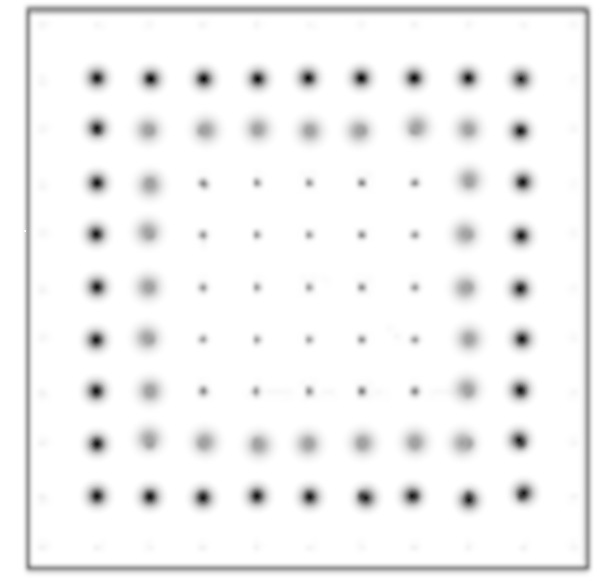
\includegraphics[width=0.5\textwidth]{./Figuras/malla.png}
\caption{Malla de puntos que resalta las fronteras, los puntos más oscuros representan una frontera \emph{fantasma}, es decir, ese conjunto de puntos estará allí como apoyo para resolver los cálculos que hará la computadora, dado que tanto el método de Lax, como el método de HLL usan los puntos posteriores y anteriores en el espacio del punto que queremos saber su valor, pero no se graficarán.} \label{fig: malla de puntos}
\end{figure}

La Figura \ref{fig: malla de puntos} muestra 
los puntos más negros como unos puntos que nos van a 
servir de apoyo para calcular los valores de los puntos más grises, esto debido a que para calcular 
los valores de algún punto $(x_i, y_j)$ necesitamos el punto posterior $x_{i+1}, y_{j+1}$ y el punto 
anterior $x_{i-1}, y_{j-1}$.

Ahora, cuando llegamos a los últimos puntos de nuestra frontera, 
por ejemplo, el punto $x_{0}, y_{0}$, no podremos calcularlo debido a que  no tendremos conocimiento acerca del punto anterior $x_{(-1)}, y_{(-1)}$, entonces  tendremos que darles valores específicos a estos puntos, pero no podemos darles cualquier valor, en las siguientes secciones vamos a ver que valores válidos le podemos dar para el funcionamiento del código. 

%----------------------------------------------------------------------------------------------
\subsection{Condiciones de frontera \emph{outflow}}
%----------------------------------------------------------------------------------------------
Las condiciones \emph{outflow}, son en las que los valores de nuestra frontera fantasma(puntos negros) que toman los  mismos valores que su antecesor (puntos grises), los fenómenos físicos que atraviesan nuestra frontera, pasarán como si tuviéramos más dominio hacia afuera y una vez que salgan perderemos información sobre esta.

\begin{figure}[H]
\centering
\subfigure[onda expandiéndose antes de cruzar la frontera]{\includegraphics[scale = 0.50]{./Figuras/Apendice/outflow1}}
\subfigure[onda expandiéndose después de cruzar la frontera]{\includegraphics[scale = 0.50]{./Figuras/Apendice/outflow2}}
\caption{Al pasar la onda nuestra frontera, esta sigue su trayecto normal como si el dominio fuera infinito} \label{fig:reflexion}
\end{figure}

Las ecuaciones que obedece nuestra frontera son las siguientes:
\begin{eqnarray}
\textbf{U}(0,j)&=&\textbf{U}(1,j) \\
\textbf{U}(n+1,j)&=&\textbf{U}(n,j) \\
\textbf{U}(i,0)&=&\textbf{U}(i,1) \\
\textbf{U}(i,m+1)&=&\textbf{U}(i,m) 
\end{eqnarray}

Donde $i,j \leq n,m \in \mathbb{N}$

%----------------------------------------------------------------------------------------------
\subsection{Condiciones de frontera \emph{reflexión}}
%----------------------------------------------------------------------------------------------
Las condiciones de reflexión funcionan como una pared en la que no se le permite al fenómeno físico escapar y al toparse con estas fronteras se reflejarán. Los valores que tendrán los puntos negros, serán los valores negativos de los puntos grises.

\begin{figure}[H]
\centering
\subfigure[onda expandiéndose antes de llegar a la frontera]{\includegraphics[scale = 0.50]{./Figuras/Apendice/reflexion1}}
\subfigure[onda reflejándose en las fronteras]{\includegraphics[scale = 0.50]{./Figuras/Apendice/reflexion2}}
\caption{Al llegar la frontera la onda se reflejará y chocará con la misma} \label{fig:reflexion}
\end{figure}

Las ecuaciones que obedece nuestra frontera son las siguientes:
\begin{eqnarray}
\textbf{U}(0,j)&=&-\textbf{U}(1,j) \\
\textbf{U}(n+1,j)&=&-\textbf{U}(n,j) \\
\textbf{U}(i,0)&=&-\textbf{U}(i,1) \\
\textbf{U}(i,m+1)&=&-\textbf{U}(i,m) 
\end{eqnarray}

%----------------------------------------------------------------------------------------------
\subsection{Condiciones de frontera \emph{periódicas}}
%----------------------------------------------------------------------------------------------
Las condiciones periódicas son cuando nuestra frontera fantasma toma los valores de la frontera opuesta del lado que están, es decir, si un fenómeno físico pasa a través de la parte de arriba de nuestro dominio (ver Figura \ref{fig:periodicas}), este, saldrá por la parte de abajo y viceversa, lo mismo aplica para los fenómenos pasen por la parte izquierda o derecha de nuestro dominio.
 
\begin{figure}[H]
\centering
\subfigure[Onda antes de tocar la frontera de abajo]{\includegraphics[scale = 0.50]{./Figuras/Apendice/periodicas1.png}}
\subfigure[La onda pasa la frontera de abajo y sale por la parte de arriba]{\includegraphics[scale = 0.50]{./Figuras/Apendice/periodicas2.png}}
\caption{Al llegar la onda abajo se puede ver que se transporta al lado de arriba, se eligió esa posición de la onda, solo para resaltar la periodicidad de la onda, ya que si se hubiera puesto en el centro, la onda chocaría contra sí mismo y no podríamos ver el paso de la onda.} \label{fig:periodicas}
\end{figure}

Las ecuaciones que representan este tipo de frontera son las siguientes:

\begin{eqnarray}
\textbf{U}(0,j)&=&\textbf{U}(n,j) \\
\textbf{U}(n+1,j)&=&\textbf{U}(1,j) \\
\textbf{U}(i,0)&=&\textbf{U}(i,m) \\
\textbf{U}(i,m+1)&=&\textbf{U}(i,1) 
\end{eqnarray}

%----------------------------------------------------------------------------------------------
\subsection{Condiciones de frontera \emph{Jet} }
%----------------------------------------------------------------------------------------------
Las condiciones de tipo jet, son en las que dado un lado de nuestra frontera (pueden ser varios), se va a inyectar una energía y masa a una cierta velocidad constante todo el tiempo en una de las partes de la frontera.

 
\begin{figure}[H]
\centering
\subfigure[La densidad del medio sin la inyección del jet]{\includegraphics[scale = 0.50]{./Figuras/Apendice/jet1.png}}
\subfigure[Jet inyectándose en el medio]{\includegraphics[scale = 0.50]{./Figuras/Apendice/jet2.png}}
\caption{El jet es básicamente inyectar masa y energía en una parte de nuestra frontera, a cada tiempo que evoluciona.} \label{fig:periodicas}
\end{figure}

Para obtener las ecuaciones de esta frontera, igualamos los valores de la frontera \emph{fantasma} con las variables primitivas de nuestro jet, las siguientes ecuaciones son para la parte de abajo de nuestro dominio.
7
No relativista

\begin{eqnarray}
\textbf{U}(1,0,j)&=&\rho_{jet} \\
\textbf{U}(2,0,j)&=& \rho_{jet} v_{x_{jet}}\\
\textbf{U}(3,0,j)&=& \rho_{jet} v_{y_{jet}}\\
\textbf{U}(4,0,j)&=& E_{jet}
\end{eqnarray}

Relativista

\begin{eqnarray}
\textbf{U}(1,0,j)&=&\rho_{jet} \gamma \\
\textbf{U}(2,0,j)&=& \rho_{jet} v_{x_{jet}} \gamma^2 h \\
\textbf{U}(3,0,j)&=& \rho_{jet} v_{y_{jet}} \gamma^2 h \\
\textbf{U}(4,0,j)&=& \rho_{jet} \gamma^2 h-P
\end{eqnarray}

donde $j\in \left[ a,b \right]$ y $a\geq 0, \, b\leq n+1$. Los puntos de la frontera que no sean del jet se pueden combinar con los 3 tipos de frontera mencionados anteriormente.

%----------------------------------------------------------------------------------------------
\chapter{Subrutina de Newton-Raphson}\label{ap_newrap}
%----------------------------------------------------------------------------------------------
Subrutina de Newton-Raphson, los valores de entrada son $m^2$ y las conservadas y devuelve $W$
\begin{lstlisting} [frame=single]
  subroutine newrap(qu, w, m2)

!    use parameters, only : neq, gamma
    use globals , only : neq, gamma
    implicit none
    ! real, intent(in) :: qu(neq)
    real, intent(in)  :: m2
    real, intent(out) :: w
    real, parameter :: eps = 1d-10
    real :: a, b, c, mu, alpha, u2, lor, chi, dpdchi, dpdrho
    real :: w0, dpdw, f, dfdw, pg, dv2dw, dchidw, drhodw, qu(neq)
    integer :: k

    !print*, qu(4)**2, m2+qu(1)**2, qu(4)

    !if(qu(4)**2 .lt. m2+qu(1)**2 .or. qu(4).le. 0.0) then !.lt. -> '<'; .le. -> '<=='
    !  print*,'error in newrap'
    !  stop
    !end if

    a = 3.0;   b = 2.0 * (-qu(4));   c = m2
    if(b**2-a*c .lt. 0.0) then
      print*,'b**2-a*c<0'
      stop
    end if
    w = ( - b + sqrt(b**2-a*c) ) / a   ! initial guess for w = rho * h * lor**2

    w0 = w
    mu = 1.0
  100 continue
    do k = 1, 40

      alpha = m2 / w**2   ! alpha < 1 !

      u2  = alpha/(1.0-alpha)

      if(u2 .lt. 0.0) then
        print*,'u2<0cc'
        print*,qu
        stop
      end if

      lor = sqrt(1.0 + u2)

      chi = (w - qu(1)*(1.0+u2/(lor+1.0)))/(1.0+u2)

      ! ideal gas case        
      pg     = (gamma - 1.0)/gamma * chi
      dpdchi = (gamma - 1.0)/gamma
      dpdrho = 0.0

      f = w - pg - qu(4)  ! f(w) = 0

      if(abs(f) .lt. eps) return

      dv2dw  = lor/w**3*m2
      dchidw = 1.0/lor**2 + dv2dw*(qu(1)+2.0*lor*chi)

      drhodw = dv2dw*qu(1)

      dpdw = dpdchi*dchidw + dpdrho*drhodw

      dfdw   = 1.0 - dpdw    ! df/dw

      w  = w0 - mu * f / dfdw                       ! Newton-Raphson iteration

      if(abs(w-w0).lt.eps) return

      w0 = w

    end do

    if(mu .gt. 0.1) then
      mu = mu/2.0
      goto 100
    end if

  end subroutine newrap

\end{lstlisting}

%----------------------------------------------------------------------------------------------
\chapter{Subrutinas de Flujos calculados mediante el método de HLL}\label{ap_subrutina_fluxesHLL}
%----------------------------------------------------------------------------------------------
\begin{lstlisting} [frame=single]
  !     !Este modulo calcula los flujos hll
      use globals
      implicit none
!     real, intent(in) :: time
    
    real, intent(out)::fhll(neq,0:nx+1,0:ny+1), ghll(neq,0:nx+1,0:ny+1)! esta es la variable que se obtiene y va para la subrutina ulax

    real :: rho_l(0:nx+1,0:ny+1), rho_r(0:nx+1,0:ny+1),rho_u(0:nx+1,0:ny+1),rho_d(0:nx+1,0:ny+1)
    real :: vx_l(0:nx+1,0:ny+1), vx_r(0:nx+1,0:ny+1), vx_u(0:nx+1,0:ny+1), vx_d(0:nx+1,0:ny+1)
    real :: vy_l(0:nx+1,0:ny+1), vy_r(0:nx+1,0:ny+1), vy_u(0:nx+1,0:ny+1), vy_d(0:nx+1,0:ny+1)
    real :: P_l(0:nx+1, 0:ny+1), P_r(0:nx+1, 0:ny+1), P_u(0:nx+1,0:ny+1), P_d(0:nx+1,0:ny+1)

    real :: lor_l(0:nx+1, 0:ny+1), lor_r(0:nx+1, 0:ny+1), lor_u(0:nx+1, 0:ny+1), lor_d(0:nx+1, 0:ny+1)
    real :: h_l(0:nx+1,0:ny+1), h_r(0:nx+1,0:ny+1), h_u(0:nx+1,0:ny+1), h_d(0:nx+1,0:ny+1)

    real ::s_l(0:nx+1,0:ny+1),s_r(0:nx+1,0:ny+1), s_d(0:nx+1,0:ny+1), s_u(0:nx+1,0:ny+1)
    
    

    real :: f_l(neq, 0:nx+1,0:ny+1), f_r(neq,0:nx+1,0:ny+1), u_l(neq,0:nx+1,0:ny+1), u_r(neq,0:nx+1,0:ny+1)
    real :: g_d(neq, 0:nx+1,0:ny+1), g_u(neq,0:nx+1,0:ny+1), u_d(neq,0:nx+1,0:ny+1), u_u(neq,0:nx+1,0:ny+1)

    integer :: i,j

    call RL(nx,ny, neq, gamma, u, rho_l,rho_d, rho_r,rho_u, vx_l,vx_d, vx_r,vx_u, &
  vy_l,vy_r,vy_u, vy_d,P_l,P_d, P_r,P_u)

    call wavespeeds(s_l,s_d, s_r,s_u,rho_l,rho_d, rho_r,rho_u, vx_l,vx_d, vx_r,vx_u, &
  vy_l,vy_r,vy_u, vy_d,P_l,P_d, P_r,P_u )

    
!       !igual calculamos los flujos y conservadas de lado derecho e izquierdo

  if(choose_rel==0)then
  
      do i=1,nx
        do j=1,ny
          u_l(1,i,j) = rho_l(i,j)
          u_l(2,i,j) = rho_l(i,j)*vx_l(i,j)
          u_l(3,i,j) = rho_l(i,j)*vy_l(i,j)
          u_l(4,i,j) = 0.5*rho_l(i,j)*(vx_l(i,j)**2+vy_l(i,j)**2)+P_l(i,j)/(gamma-1.)

          u_d(1,i,j) = rho_d(i,j)
          u_d(2,i,j) = rho_d(i,j)*vx_d(i,j)
          u_d(3,i,j) = rho_d(i,j)*vy_d(i,j)
          u_d(4,i,j) = 0.5*rho_d(i,j)*(vx_d(i,j)**2+vy_d(i,j)**2)+P_d(i,j)/(gamma-1.)

          u_r(1,i,j) = rho_r(i,j)
          u_r(2,i,j) = rho_r(i,j)*vx_r(i,j)
          u_r(3,i,j) = rho_r(i,j)*vy_r(i,j)
          u_r(4,i,j) = 0.5*rho_r(i,j)*(vx_r(i,j)**2+vy_r(i,j)**2)+P_r(i,j)/(gamma-1.)

          u_u(1,i,j) = rho_u(i,j)
          u_u(2,i,j) = rho_u(i,j)*vx_u(i,j)
          u_u(3,i,j) = rho_u(i,j)*vy_u(i,j)
          u_u(4,i,j) = 0.5*rho_u(i,j)*(vx_u(i,j)**2+vy_u(i,j)**2)+P_u(i,j)/(gamma-1.)

!========================================================

          f_l(1,i,j) = rho_l(i,j)*vx_l(i,j)
          f_l(2,i,j) = rho_l(i,j)*vx_l(i,j)**2+P_l(i,j)
          f_l(3,i,j) = rho_l(i,j)*vx_l(i,j)*vy_l(i,j)
          f_l(4,i,j) = vx_l(i,j)*(u_l(4,i,j)+P_l(i,j))

          f_r(1,i,j) = rho_r(i,j)*vx_r(i,j)
          f_r(2,i,j) = rho_r(i,j)*vx_r(i,j)**2+P_r(i,j)
          f_r(3,i,j) = rho_r(i,j)*vx_r(i,j)*vy_r(i,j)
          f_r(4,i,j) = vx_r(i,j)*(u_r(4,i,j)+P_r(i,j))

          g_d(1,i,j) = rho_d(i,j)*vy_d(i,j)
          g_d(2,i,j) = rho_d(i,j)*vx_d(i,j)*vy_d(i,j)
          g_d(3,i,j) = rho_d(i,j)*vy_d(i,j)**2 + P_d(i,j)
          g_d(4,i,j) = vy_d(i,j)*(u_d(4,i,j)+P_d(i,j))

          g_u(1,i,j) = rho_u(i,j)*vy_u(i,j)
          g_u(2,i,j) = rho_u(i,j)*vx_u(i,j)*vy_u(i,j)
          g_u(3,i,j) = rho_u(i,j)*vy_u(i,j)**2 + P_u(i,j)
          g_u(4,i,j) = vy_u(i,j)*(u_u(4,i,j)+P_u(i,j))

        end do
      end do

  elseif(choose_rel==1)then

      do i=1,nx
        do j=1,ny

          lor_l(i,j) = 1/sqrt(1-(vx_l(i,j)**2+vy_l(i,j)**2))
          lor_d(i,j) = 1/sqrt(1-(vx_d(i,j)**2+vy_d(i,j)**2))
          lor_r(i,j) = 1/sqrt(1-(vx_r(i,j)**2+vy_r(i,j)**2))
          lor_u(i,j) = 1/sqrt(1-(vx_u(i,j)**2+vy_u(i,j)**2))

          h_l(i,j)=1.+gamma/(gamma-1.)*P_l(i,j)/rho_l(i,j)
          h_d(i,j)=1.+gamma/(gamma-1.)*P_d(i,j)/rho_d(i,j)
          h_r(i,j)=1.+gamma/(gamma-1.)*P_r(i,j)/rho_r(i,j)
          h_u(i,j)=1.+gamma/(gamma-1.)*P_u(i,j)/rho_u(i,j)

          u_l(1,i,j) = rho_l(i,j)*lor_l(i,j)
          u_l(2,i,j) = rho_l(i,j)*vx_l(i,j)*lor_l(i,j)**2*h_l(i,j)
          u_l(3,i,j) = rho_l(i,j)*vy_l(i,j)*lor_l(i,j)**2*h_l(i,j)
          u_l(4,i,j) = rho_l(i,j)*lor_l(i,j)**2*h_l(i,j)-P_l(i,j)

          u_d(1,i,j) = rho_d(i,j)*lor_d(i,j)
          u_d(2,i,j) = rho_d(i,j)*vx_d(i,j)*lor_d(i,j)**2*h_d(i,j)
          u_d(3,i,j) = rho_d(i,j)*vy_d(i,j)*lor_d(i,j)**2*h_d(i,j)
          u_d(4,i,j) = rho_d(i,j)*lor_d(i,j)**2*h_d(i,j)-P_d(i,j)

          u_r(1,i,j) = rho_r(i,j)*lor_r(i,j)
          u_r(2,i,j) = rho_r(i,j)*vx_r(i,j)*lor_r(i,j)**2*h_r(i,j)
          u_r(3,i,j) = rho_r(i,j)*vy_r(i,j)*lor_r(i,j)**2*h_r(i,j)
          u_r(4,i,j) = rho_r(i,j)*lor_r(i,j)**2*h_r(i,j)-P_r(i,j)

          u_u(1,i,j) = rho_u(i,j)*lor_u(i,j)
          u_u(2,i,j) = rho_u(i,j)*vx_u(i,j)*lor_u(i,j)**2*h_u(i,j)
          u_u(3,i,j) = rho_u(i,j)*vy_u(i,j)*lor_u(i,j)**2*h_u(i,j)
          u_u(4,i,j) = rho_u(i,j)*lor_u(i,j)**2*h_u(i,j)-P_u(i,j)

!==========================================================================

          f_l(1,i,j) = rho_l(i,j)*vx_l(i,j)*lor_l(i,j)
          f_l(2,i,j) = rho_l(i,j)*vx_l(i,j)**2*lor_l(i,j)**2*h_l(i,j)+P_l(i,j)
          f_l(3,i,j) = rho_l(i,j)*vx_l(i,j)*vy_l(i,j)*lor_l(i,j)**2*h_l(i,j)
          f_l(4,i,j) = rho_l(i,j)*vx_l(i,j)*lor_l(i,j)**2*h_l(i,j)

          f_r(1,i,j) = rho_r(i,j)*vx_r(i,j)*lor_r(i,j)
          f_r(2,i,j) = rho_r(i,j)*vx_r(i,j)**2*lor_r(i,j)**2*h_r(i,j)+P_r(i,j)
          f_r(3,i,j) = rho_r(i,j)*vx_r(i,j)*vy_r(i,j)*lor_r(i,j)**2*h_r(i,j)
          f_r(4,i,j) = rho_r(i,j)*vx_r(i,j)*lor_r(i,j)**2*h_r(i,j)

          g_d(1,i,j) = rho_d(i,j)*vy_d(i,j)*lor_d(i,j)
          g_d(2,i,j) = rho_d(i,j)*vx_d(i,j)*vy_d(i,j)*lor_d(i,j)**2*h_d(i,j)
          g_d(3,i,j) = rho_d(i,j)*vy_d(i,j)**2*lor_d(i,j)**2*h_d(i,j)+P_d(i,j)
          g_d(4,i,j) = rho_d(i,j)*vy_d(i,j)*lor_d(i,j)**2*h_d(i,j)

          g_u(1,i,j) = rho_u(i,j)*vy_u(i,j)*lor_u(i,j)
          g_u(2,i,j) = rho_u(i,j)*vx_u(i,j)*vy_u(i,j)*lor_u(i,j)**2*h_u(i,j)
          g_u(3,i,j) = rho_u(i,j)*vy_u(i,j)**2*lor_u(i,j)**2*h_u(i,j)+P_u(i,j)
          g_u(4,i,j) = rho_u(i,j)*vy_u(i,j)*lor_u(i,j)**2*h_u(i,j)

        end do
      end do

  endif

      do i=1,nx
        do j=1,ny
          
          if (0 .le. s_l(i,j)) then !less or equal 0<=sl
            fhll(:,i,j)=f_l(:, i,j)

          else if (s_l(i,j) .le. 0 .and. 0 .le. s_r(i,j)) then !sl<=0<=sr
        
            fhll(:,i,j)=(s_r(i,j)*f_l(:,i,j)-s_l(i,j)*f_r(:,i,j)+s_l(i,j)*s_r(i,j)*(u_r(:,i,j)-u_l(:,i,j)))/&
            (s_r(i,j)-s_l(i,j))

      
          else if (s_r(i,j) .le. 0) then !sr<=0
              fhll(:,i,j)=f_r(:,i,j)

          endif

          if(0 .le. s_d(i,j)) then
            ghll(:,i,j)= g_d(:,i,j)

          else if(s_d(i,j) .le. 0 .and. 0 .le. s_u(i,j)) then

            ghll(:,i,j)=(s_u(i,j)*g_d(:,i,j)-s_d(i,j)*g_u(:,i,j)+s_d(i,j)*s_u(i,j)*(u_u(:,i,j)-u_d(:,i,j)))/&
            (s_u(i,j)-s_d(i,j))

          else if(s_u(i,j) .le. 0) then
              ghll(:,i,j) = g_u(:,i,j)

          endif
        end do
      end do

  fhll(:,nx+1,:) = fhll(:,nx-1,:)
!   fhll(:,nx,:)   = fhll(:,nx-1,:)     
  fhll(:,0,:)    = fhll(:,2,:)
!   fhll(:,1,:)    = fhll(:,2,:)     
  fhll(:,:,ny+1) = fhll(:,:,ny-1)
!   fhll(:,:,ny)   = fhll(:,:,ny-1)
  fhll(:,:,0)    = fhll(:,:,2)
!   fhll(:,:,1)    = fhll(:,:,2)

  ghll(:,nx+1,:) = ghll(:,nx-1,:)
!   ghll(:,nx,:)   = ghll(:,nx-1,:)     
  ghll(:,0,:)    = ghll(:,2,:)
!   ghll(:,1,:)    = ghll(:,2,:)     
  ghll(:,:,ny+1) = ghll(:,:,ny-1)
!   ghll(:,:,ny)   = ghll(:,:,ny-1)
  ghll(:,:,0)    = ghll(:,:,2)
!   ghll(:,:,1)    = ghll(:,:,2)

  return


\end{lstlisting}

%----------------------------------------------------------------------------------------------
\begin{thebibliography}{40}
%----------------------------------------------------------------------------------------------

% \bibitem{Berger:2013jza} 
%   E.~Berger,
%   Short-Duration Gamma-Ray Bursts,
%   Ann.\ Rev.\ Astron.\ Astrophys.\  {\bf 52}, 43 (2014)
%   doi:10.1146/annurev-astro-081913-035926
%   [arXiv:1311.2603 [astro-ph.HE]].
%   %%CITATION = doi:10.1146/annurev-astro-081913-035926;%%
%   %424 citations counted in INSPIRE as of 02 Jan 2019
 
% %\bibitem{2012ApJ...760..122G} Gao, Y., \& Law, C.~K.\ 2012, \apj , 760, 122

\bibitem[Mignone \& Bodo (2005)]{MB-HLLC-I}Mignone, A., Bodo, G., 2005. An HLLC Riemann solver for relativistic flows -- I. Hydrodynamics. Monthly Notices of the Royal Astronomical Society 364, 126–136. doi:10.1111/j.1365-2966.2005.09546.x 

\bibitem[Dal Pino (2004)]{deGouveiaDalPino:2004jy} de Gouveia Dal Pino, E.M., 2005. Astrophysical Jets and outflows. Advances in Space Research 35, 908–924. doi:10.1016/j.asr.2005.03.145 

\bibitem[Blandford et al.(2019)]{2019ARA&A..57..467B} Blandford, R., Meier, D., Readhead, A., 2019. Relativistic jets from active galactic nuclei. Annual Review of Astronomy and Astrophysics 57, 467–509. doi:10.1146/annurev-astro-081817-051948 

\bibitem[Espinasse et al.(2020)]{2020ApJ...895L..31E} Espinasse, M., Corbel, S., Kaaret, P., Tremou, E., Migliori, G., Plotkin, R.M., Bright, J., Tomsick, J., Tzioumis, A., Fender, R., Orosz, J.A., Gallo, E., Homan, J., 
Jonker, P.G., Miller-Jones, J.C., Russell, D.M., Motta, S., 2020. Relativistic X-ray jets from the black hole X-ray binary maxi J1820+070. The Astrophysical Journal 895. doi:10.3847/2041-8213/ab88b6 

\bibitem[Pavan et al.(2021)]{2021MNRAS.506.3483P} Pavan, A., Ciolfi, R., Kalinani, J.V., Mignone, A., 2021. Short gamma-ray burst jet propagation in binary neutron star merger environments. Monthly Notices of the Royal Astronomical Society 506, 
3483–3498. doi:10.1093/mnras/stab1810 

\bibitem[Shrestha et al.(2022)]{2022MNRAS.509.5964S} Shrestha, M., Steele, I.A., Kobayashi, S., Jordana-Mitjans, N., Smith, R.J., Jermak, H., Arnold, D., Mundell, C.G., Gomboc, A., Guidorzi, C., 2021. GRB 191016a: A highly collimated gamma-ray 
burst jet with magnetized energy injection. Monthly Notices of the Royal Astronomical Society 509, 5964–5973. doi:10.1093/mnras/stab3368 


\bibitem[Blandford \& Znajek(1977)]{1977MNRAS.179..433B} Blandford, R.D., Znajek, R.L., 1977. Electromagnetic extraction of energy from Kerr Black holes. Monthly Notices of the Royal Astronomical Society 179, 433–456. 
doi:10.1093/mnras/179.3.433 

\bibitem[Blandford \& Payne(1982)]{1982MNRAS.199..883B} Blandford, R.D., Payne, D.G., 1982. Hydromagnetic flows from accretion discs and the production of Radio Jets. Monthly Notices of the Royal Astronomical Society 199, 883–903. 
doi:10.1093/mnras/199.4.883 

\bibitem[H{\"u}lss and Wiebusch(2008)]{2008ICRC....5.1405H} H{\"u}lss, J.-P., Wiebusch, C.\ 2008.\ Search for Signatures of Extra-Terrestrial Neutrinos with a Multipole Analysis of the AMANDA-II 
Sky-map.\ International Cosmic Ray Conference 5, 1405–1408.

\bibitem[Romero (2021)]{2021Romero} Romero, G.E., 2021. The content of Astrophysical Jets. Astronomische Nachrichten 342, 727–734. doi:10.1002/asna.202113989 

\bibitem[T. Pirán (2005)]{PGRB-piran} Piran, T., 2005. The physics of gamma-ray bursts. Reviews of Modern Physics 76, 1143–1210. doi:10.1103/revmodphys.76.1143 

\bibitem[Zhang, B. (2018)]{Zhang:PGRB}
Zhang, B. (2018). GRB Phenomenology. In The Physics of Gamma-Ray Bursts (pp. 27-121). Cambridge: Cambridge University Press. doi:10.1017/9781139226530.004
% % 2019-The Physics of Gamma-Ray Bursts.pdf

\bibitem[Berger (2014)]{Berger:2014jza}Berger, E., 2014. Short-duration gamma-ray bursts. Annual Review of Astronomy and Astrophysics 52, 43–105. doi:10.1146/annurev-astro-081913-035926 

\bibitem[Seo et al. (2021)]{Seo2021}Seo, J., Kang, H., Ryu, D., Ha, S., Chattopadhyay, I., 2021. A simulation study of ultra-relativistic jets–I. A new code for relativistic hydrodynamics. 
The Astrophysical Journal 920, 143. doi:10.3847/1538-4357/ac19b3 

\bibitem[Perucho et al.(2011)]{2011ApJ...743...42P} Perucho, M., Quilis, V., Martí, J.-M., 2011. Intracluster medium reheating by Relativistic Jets. The Astrophysical Journal 743, 42. doi:10.1088/0004-637x/743/1/42 

\bibitem[L{\'o}pez-C{\'a}mara et al.(2013)]{2013ApJ...767...19L} López-Cámara, D., Morsony, B.J., Begelman, M.C., Lazzati, D., 2013. Three-dimensional adaptive mesh refinement simulations of long-duration gamma-ray 
burst jets inside massive progenitor stars. The Astrophysical Journal 767, 19. doi:10.1088/0004-637x/767/1/19

\bibitem[Lazzati et al.(2018)]{2018PhRvL.120x1103L} Lazzati, D., Perna, R., Morsony, B.J., Lopez-Camara, D., Cantiello, M., Ciolfi, R., Giacomazzo, B., Workman, J.C., 2018. Late time afterglow observations reveal a 
collimated relativistic jet in the ejecta of the binary neutron star Merger GW170817. Physical Review Letters 120. doi:10.1103/physrevlett.120.241103 

\bibitem[Gottlieb et al.(2021)]{2021MNRAS.500.3511G} Gottlieb, O., Nakar, E., Bromberg, O., 2020. The structure of hydrodynamic $\gamma$-Ray Burst Jets. Monthly Notices of the Royal Astronomical Society 500, 3511–3526. 
doi:10.1093/mnras/staa3501 

\bibitem[De Colle et al.(2012)]{2012ApJ...751...57D} De Colle, F., Ramirez-Ruiz, E., Granot, J., Lopez-Camara, D., 2012. Simulations of gamma-ray burst jets in a stratified external medium: Dynamics, afterglow light 
curves, jet breaks, and radio calorimetry. The Astrophysical Journal 751, 57. doi:10.1088/0004-637x/751/1/57 

\bibitem[Hamidani \& Ioka (2020)]{JBEMGRB} Hamidani, H., Ioka, K., 2020. Jet propagation in expanding medium for gamma-ray bursts. Monthly Notices of the Royal Astronomical Society 500, 627–642. doi:10.1093/mnras/staa3276 

\bibitem[Clarke \& Carswell (2007)]{PAFD}
Clarke, C., Carswell, B., 2007. Blast waves. Principles of Astrophysical Fluid Dynamics 89–106. doi:10.1017/cbo9780511813450.009 
% %Cathie Clarke, Bob Carswell - Principles of astrophysical fluid dynamics (2007, Cambridge University Press).pdf

\bibitem[LeVeque et al. (1998)]{LeVeque1998}LeVeque, R.J., Steiner, O., Gautschy, A., 1998. Nonlinear Conservation Laws and Finite Volume Methods, in: Computational Methods for Astrophysical Fluid Flow. Springer, Berlin, pp. 1–148. 

\bibitem[Clarke et al. (2007)]{Clarke2007}Clarke, C., \& Carswell, B. (2007). The fluid equations. In Principles of Astrophysical Fluid Dynamics (pp. 12-19). 
Cambridge: Cambridge University Press. doi:10.1017/CBO9780511813450.003

\bibitem[Martí \& Müller (1999)]{Marty1999}Martí, J.M., Müller, E., 1999. Numerical hydrodynamics in special relativity. Living Reviews in Relativity 2. doi:10.12942/lrr-1999-3

\bibitem[Duran (2010)]{Duran2021}Durran, D.R. (2010). Finite-Difference Approximations for One-Dimensional Transport. In: Numerical Methods for Fluid Dynamics. Texts in Applied Mathematics, 
vol 32. Springer, New York, NY. https://doi.org/10.1007/978-1-4419-6412-0\_3

\bibitem[Toro (1997)]{Toro1997} Toro E.F. (1997) The HLL and HLLC Riemann Solvers. In: Riemann Solvers and Numerical Methods for Fluid Dynamics. Springer, Berlin, Heidelberg

\bibitem[Duchateau et al. (2002)]{Duchateau2002}Duchateau, P., Zachmann, D.W., 2002. Applied partial differential equations. Dover, Mineola, NY.

\bibitem[Prunty (2019)]{Prunty2019}Prunty, S. (2019). Conditions Across the Shock: The Rankine-Hugoniot Equations. In: Introduction to Simple Shock Waves in Air . Shock Wave and High Pressure Phenomena. Springer, Cham. https://doi.org/10.1007/978-3-030-02565-6\_3

\bibitem[Landau \& Lifshitz (1987)]{Landau1987}Landau Lev Davidovic, Lifsic, E.M., 514, 505, 1987. RELATIVISTIC FLUID DYNAMICS, in: 6: Fluid Mechanics. Butterworth-Heinemann, Oxford.

\bibitem[Lora et al. (2013)]{Lora2013}
F.D. Lora-Clavijo \emph(et. al.) (2013). Exact Solution oh the 1D riemann problem in Newtonian and relativistic hydrodynamics. Revista Mexicana de Física. E 59 (2013)28-50 

\bibitem[Martí (2019)]{Marti2019}
Martí, J.-M., 2019. Numerical simulations of jets from active galactic nuclei. Galaxies 7, 24. doi:10.3390/galaxies7010024l simulations of jets from active galactic nuclei. Galaxies 7, 24. doi:10.3390/galaxies7010024

\bibitem[Mignone \& McKinney (2007)]{McKinney2007}Mignone, A., McKinney, J.C., 2007. Equation of state in relativistic magnetohydrodynamics: Variable versus constant adiabatic index. Monthly Notices of the 
Royal Astronomical Society 378, 1118-1130. doi:10.1111/j.1365-2966.2007.11849.x 


 



% \bibitem{MB-HLLC-RSfRF}
% A. Mignone, G. Bodo, An HLLC Riemann solver for relativistic flows – II. Magnetohydrodynamics, Monthly Notices of the Royal Astronomical Society, Volume 368, Issue 3, May 2006, Pages 1040–1054, https://doi.org/10.1111/j.1365-2966.2006.10162.x
% %0601640.pdf


% \bibitem{Decade-sgrb}
% Fong, W. et al. “A DECADE OF SHORT-DURATION GAMMA-RAY BURST BROADBAND AFTERGLOWS: ENERGETICS, CIRCUMBURST DENSITIES, AND JET OPENING ANGLES.” The Astrophysical Journal 815.2 (2015): 102. Crossref. Web.
% %1509.02922.pdf

% \bibitem{Ecasgrb}
% Teboul, O \& Piran, T. (2017). Emission of cocoon afterglow for short Gamma Ray Burst : a counterpart of gravitational waves?. 


% \bibitem{GRB:CAP}
% Azzam, W.J. \& Zitouni, Hannachi \& Guessoum, Nidhal. (2017). Gamma-Ray Bursts: Characteristics and Prospects. Journal of Physics: Conference Series. 869. 012065. 10.1088/1742-6596/869/1/012065. 
% %Azzam_2017_J._Phys.__Conf._Ser._869_012065.pdf

% \bibitem{GRB:PPP}
% ZHANG, BING, and PETER MÉSZÁROS. “GAMMA-RAY BURSTS: PROGRESS, PROBLEMS \& PROSPECTS.” International Journal of Modern Physics A 19.15 (2004): 2385–2472. Crossref. Web.
% %zhang2004.pdf



% \bibitem{PSGRB}
% Lee, William H, and Enrico Ramirez-Ruiz. “The Progenitors of Short Gamma-Ray Bursts.” New Journal of Physics 9.1 (2007): 17–17. Crossref. Web.
% %lee2007.pdf

% \bibitem{PGRB-RJ}
% Kumar, Pawan, and Bing Zhang. “The Physics of Gamma-Ray Bursts \& Relativistic Jets.” Physics Reports 561 (2015): 1–109. Crossref. Web.
% %kumar2015.pdf

% \bibitem{GRB-SE}
% Gehrels, N., E. Ramirez-Ruiz, and D.B. Fox. “Gamma-Ray Bursts in theSwiftEra.” Annual Review of Astronomy and Astrophysics 47.1 (2009): 567–617. Crossref. Web.
% %gehrels2009.pdf

% \bibitem{PNCCA}
% Mignone, A. et al. “PLUTO: A Numerical Code for Computational Astrophysics.” The Astrophysical Journal Supplement Series 170.1 (2007): 228–242. Crossref. Web.
% %Mignone_2007_ApJS_170_228.pdf

% \bibitem{GRB-levan}
% Levan, Andrew et al. “Gamma-Ray Burst Progenitors.” Space Science Reviews 202.1-4 (2016): 33–78. Crossref. Web.
% %Levan2016_Article_Gamma-RayBurstProgenitors.pdf

% \bibitem{Diego}
% Lazzati, Davide et al. “Off-Axis Prompt X-Ray Transients from the Cocoon of Short Gamma-Ray Bursts.” The Astrophysical Journal 848.1 (2017): L6. Crossref. Web.
% %Lazzati_2017_ApJL_848_L6.pdf

% \bibitem{RHRRC}
% Gao, Yang, and Chung K. Law. “RANKINE-HUGONIOT RELATIONS IN RELATIVISTIC COMBUSTION WAVES.” The Astrophysical Journal 760.2 (2012): 122. Crossref. Web.
% %Gao_2012_ApJ_760_122.pdf

% \bibitem{1973ApJ...179..897T} Thorne, K.~S.\ 1973.\ Relativistic Shocks: the Taub Adiabat.\ The Astrophysical Journal 179, 897.
% %1973ApJ...179..897T.pdf



% \bibitem{SGRBr-Avanzo}
% D'Avanzo, P.. (2015). Short gamma ray bursts: A review. Journal of High Energy Astrophysics. 7. 10.1016/j.jheap.2015.07.002. 























% % \bibitem[Pino (2004)]{deGouveiaDalPino:2004jy}
% % E.~M.~de Gouveia Dal Pino,
% % %``Astrophysical jets and outflows,''
% % Adv. Space Res. \textbf{35} (2005), 908
% % doi:10.1016/j.asr.2005.03.145
% % [arXiv:astro-ph/0406319 [astro-ph]].
% %31 citations counted in INSPIRE as of 03 May 2022




%----------------------------------------------------------------------------------------------
\end{thebibliography}
%----------------------------------------------------------------------------------------------
\end{document}
%----------------------------------------------------------------------------------------------
%----------------------------------------------------------------------------------------------